\begin{frame}{BFS : Example}
\begin{figure}
\vspace*{-1cm} 
\center
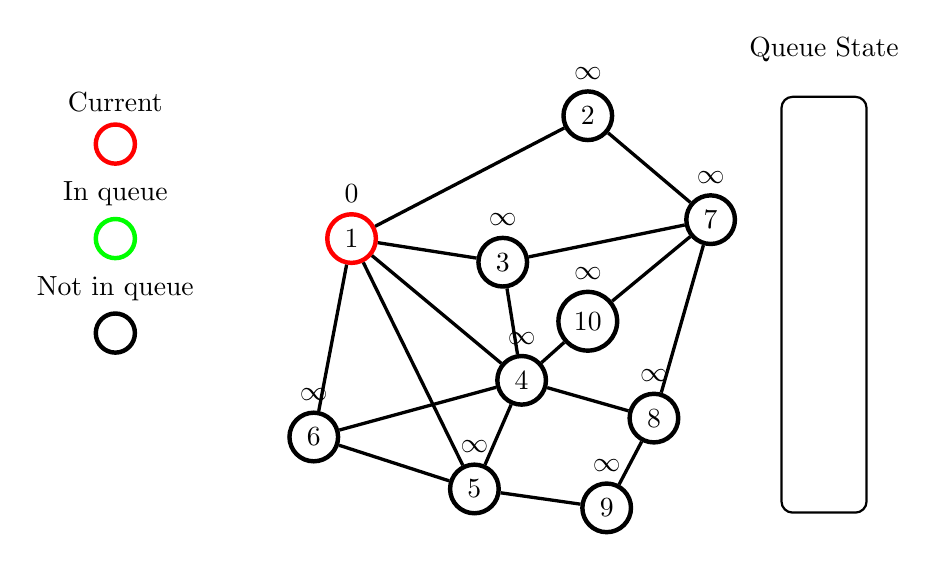
\begin{tikzpicture}[scale=1.2] 
\node[shape=circle, draw=red, 	ultra thick, scale=1.5pt, label={Current}] (U) at (-2.5, 1) {}; 
\node[shape=circle, draw=green,  ultra thick, scale=1.5pt, label={In queue}] (U) at (-2.5, 0) {}; 
\node[shape=circle, draw=black, ultra thick, scale=1.5pt, label={Not in queue}] (U) at (-2.5, -1) {}; 
\draw[thick, rounded corners,draw=black] (4.55, 1.5) rectangle ++(0.9, -1-4*0.85 );
\node[draw=white] at (5, 2) {Queue State} ; 
\node[shape=circle,draw=red, ultra thick, label={$0$}] (1) at (0,0) {1}; 
\node[shape=circle,draw=black, ultra thick, label={$\infty$}] (2) at (2.5,1.3) {2}; 
\node[shape=circle,draw=black, ultra thick, label={$\infty$}] (3) at (1.6,-0.25) {3}; 
\node[shape=circle,draw=black, ultra thick, label={$\infty$}] (4) at (1.8,-1.5) {4}; 
\node[shape=circle,draw=black, ultra thick, label={$\infty$}] (5) at (1.3,-2.65) {5}; 
\node[shape=circle,draw=black, ultra thick, label={$\infty$}] (6) at (-0.4,-2.1) {6}; 
\node[shape=circle,draw=black, ultra thick, label={$\infty$}] (7) at (3.8,0.2) {7}; 
\node[shape=circle,draw=black, ultra thick, label={$\infty$}] (8) at (3.2,-1.9) {8}; 
\node[shape=circle,draw=black, ultra thick, label={$\infty$}] (9) at (2.7,-2.85) {9}; 
\node[shape=circle,draw=black, ultra thick, label={$\infty$}] (10) at (2.5,-0.875) {10}; 
\path [-,very thick, draw=black] (1) edge  (2);
\path [-,very thick, draw=black] (1) edge  (3);
\path [-,very thick, draw=black] (1) edge  (4);
\path [-,very thick, draw=black] (1) edge  (5);
\path [-,very thick, draw=black] (1) edge  (6);
\path [-,very thick, draw=black] (2) edge  (7);
\path [-,very thick, draw=black] (3) edge  (7);
\path [-,very thick, draw=black] (3) edge  (4);
\path [-,very thick, draw=black] (4) edge  (5);
\path [-,very thick, draw=black] (4) edge  (6);
\path [-,very thick, draw=black] (4) edge  (8);
\path [-,very thick, draw=black] (4) edge  (10);
\path [-,very thick, draw=black] (5) edge  (6);
\path [-,very thick, draw=black] (5) edge  (9);
\path [-,very thick, draw=black] (7) edge  (8);
\path [-,very thick, draw=black] (7) edge  (10);
\path [-,very thick, draw=black] (8) edge  (9);
\end{tikzpicture} 
\end{figure} 
\end{frame} 
\begin{frame}{BFS : Example}
\begin{figure}
\vspace*{-1cm} 
\center
\begin{tikzpicture}[scale=1.2] 
\node[shape=circle, draw=red, 	ultra thick, scale=1.5pt, label={Current}] (U) at (-2.5, 1) {}; 
\node[shape=circle, draw=green,  ultra thick, scale=1.5pt, label={In queue}] (U) at (-2.5, 0) {}; 
\node[shape=circle, draw=black, ultra thick, scale=1.5pt, label={Not in queue}] (U) at (-2.5, -1) {}; 
\draw[thick, rounded corners,draw=black] (4.55, 1.5) rectangle ++(0.9, -1-4*0.85 );
\node[draw=white] at (5, 2) {Queue State} ; 
\node[shape=circle, draw=black, thick, minimum size=2pt] (U0) at (5, 1.0) {\tiny{2}}; 
\path[->, thick, draw=black] (2) edge [dashed, bend right=30] (U0); 
\node[shape=circle,draw=red, ultra thick, label={$0$}] (1) at (0,0) {1}; 
\node[shape=circle,draw=green, ultra thick, label={$1$}] (2) at (2.5,1.3) {2}; 
\node[shape=circle,draw=black, ultra thick, label={$\infty$}] (3) at (1.6,-0.25) {3}; 
\node[shape=circle,draw=black, ultra thick, label={$\infty$}] (4) at (1.8,-1.5) {4}; 
\node[shape=circle,draw=black, ultra thick, label={$\infty$}] (5) at (1.3,-2.65) {5}; 
\node[shape=circle,draw=black, ultra thick, label={$\infty$}] (6) at (-0.4,-2.1) {6}; 
\node[shape=circle,draw=black, ultra thick, label={$\infty$}] (7) at (3.8,0.2) {7}; 
\node[shape=circle,draw=black, ultra thick, label={$\infty$}] (8) at (3.2,-1.9) {8}; 
\node[shape=circle,draw=black, ultra thick, label={$\infty$}] (9) at (2.7,-2.85) {9}; 
\node[shape=circle,draw=black, ultra thick, label={$\infty$}] (10) at (2.5,-0.875) {10}; 
\path [->,very thick, draw=red] (1) edge  (2);
\path [-,very thick, draw=black] (1) edge  (3);
\path [-,very thick, draw=black] (1) edge  (4);
\path [-,very thick, draw=black] (1) edge  (5);
\path [-,very thick, draw=black] (1) edge  (6);
\path [-,very thick, draw=black] (2) edge  (7);
\path [-,very thick, draw=black] (3) edge  (7);
\path [-,very thick, draw=black] (3) edge  (4);
\path [-,very thick, draw=black] (4) edge  (5);
\path [-,very thick, draw=black] (4) edge  (6);
\path [-,very thick, draw=black] (4) edge  (8);
\path [-,very thick, draw=black] (4) edge  (10);
\path [-,very thick, draw=black] (5) edge  (6);
\path [-,very thick, draw=black] (5) edge  (9);
\path [-,very thick, draw=black] (7) edge  (8);
\path [-,very thick, draw=black] (7) edge  (10);
\path [-,very thick, draw=black] (8) edge  (9);
\end{tikzpicture} 
\end{figure} 
\end{frame} 
\begin{frame}{BFS : Example}
\begin{figure}
\vspace*{-1cm} 
\center
\begin{tikzpicture}[scale=1.2] 
\node[shape=circle, draw=red, 	ultra thick, scale=1.5pt, label={Current}] (U) at (-2.5, 1) {}; 
\node[shape=circle, draw=green,  ultra thick, scale=1.5pt, label={In queue}] (U) at (-2.5, 0) {}; 
\node[shape=circle, draw=black, ultra thick, scale=1.5pt, label={Not in queue}] (U) at (-2.5, -1) {}; 
\draw[thick, rounded corners,draw=black] (4.55, 1.5) rectangle ++(0.9, -1-4*0.85 );
\node[draw=white] at (5, 2) {Queue State} ; 
\node[shape=circle, draw=black, thick, minimum size=2pt] (U0) at (5, 1.0) {\tiny{2}}; 
\node[shape=circle, draw=black, thick, minimum size=2pt] (U1) at (5, 0.15000000000000002) {\tiny{3}}; 
\path[->] (U1) edge [out=75, in=-75] (U0);
\path[->, thick, draw=black] (3) edge [dashed, bend right=30] (U1); 
\node[shape=circle,draw=red, ultra thick, label={$0$}] (1) at (0,0) {1}; 
\node[shape=circle,draw=green, ultra thick, label={$1$}] (2) at (2.5,1.3) {2}; 
\node[shape=circle,draw=green, ultra thick, label={$1$}] (3) at (1.6,-0.25) {3}; 
\node[shape=circle,draw=black, ultra thick, label={$\infty$}] (4) at (1.8,-1.5) {4}; 
\node[shape=circle,draw=black, ultra thick, label={$\infty$}] (5) at (1.3,-2.65) {5}; 
\node[shape=circle,draw=black, ultra thick, label={$\infty$}] (6) at (-0.4,-2.1) {6}; 
\node[shape=circle,draw=black, ultra thick, label={$\infty$}] (7) at (3.8,0.2) {7}; 
\node[shape=circle,draw=black, ultra thick, label={$\infty$}] (8) at (3.2,-1.9) {8}; 
\node[shape=circle,draw=black, ultra thick, label={$\infty$}] (9) at (2.7,-2.85) {9}; 
\node[shape=circle,draw=black, ultra thick, label={$\infty$}] (10) at (2.5,-0.875) {10}; 
\path [-,very thick, draw=black] (1) edge  (2);
\path [->,very thick, draw=red] (1) edge  (3);
\path [-,very thick, draw=black] (1) edge  (4);
\path [-,very thick, draw=black] (1) edge  (5);
\path [-,very thick, draw=black] (1) edge  (6);
\path [-,very thick, draw=black] (2) edge  (7);
\path [-,very thick, draw=black] (3) edge  (7);
\path [-,very thick, draw=black] (3) edge  (4);
\path [-,very thick, draw=black] (4) edge  (5);
\path [-,very thick, draw=black] (4) edge  (6);
\path [-,very thick, draw=black] (4) edge  (8);
\path [-,very thick, draw=black] (4) edge  (10);
\path [-,very thick, draw=black] (5) edge  (6);
\path [-,very thick, draw=black] (5) edge  (9);
\path [-,very thick, draw=black] (7) edge  (8);
\path [-,very thick, draw=black] (7) edge  (10);
\path [-,very thick, draw=black] (8) edge  (9);
\end{tikzpicture} 
\end{figure} 
\end{frame} 
\begin{frame}{BFS : Example}
\begin{figure}
\vspace*{-1cm} 
\center
\begin{tikzpicture}[scale=1.2] 
\node[shape=circle, draw=red, 	ultra thick, scale=1.5pt, label={Current}] (U) at (-2.5, 1) {}; 
\node[shape=circle, draw=green,  ultra thick, scale=1.5pt, label={In queue}] (U) at (-2.5, 0) {}; 
\node[shape=circle, draw=black, ultra thick, scale=1.5pt, label={Not in queue}] (U) at (-2.5, -1) {}; 
\draw[thick, rounded corners,draw=black] (4.55, 1.5) rectangle ++(0.9, -1-4*0.85 );
\node[draw=white] at (5, 2) {Queue State} ; 
\node[shape=circle, draw=black, thick, minimum size=2pt] (U0) at (5, 1.0) {\tiny{2}}; 
\node[shape=circle, draw=black, thick, minimum size=2pt] (U1) at (5, 0.15000000000000002) {\tiny{3}}; 
\node[shape=circle, draw=black, thick, minimum size=2pt] (U2) at (5, -0.7) {\tiny{4}}; 
\path[->] (U1) edge [out=75, in=-75] (U0);
\path[->] (U2) edge [out=75, in=-75] (U1);
\path[->, thick, draw=black] (4) edge [dashed, bend right=30] (U2); 
\node[shape=circle,draw=red, ultra thick, label={$0$}] (1) at (0,0) {1}; 
\node[shape=circle,draw=green, ultra thick, label={$1$}] (2) at (2.5,1.3) {2}; 
\node[shape=circle,draw=green, ultra thick, label={$1$}] (3) at (1.6,-0.25) {3}; 
\node[shape=circle,draw=green, ultra thick, label={$1$}] (4) at (1.8,-1.5) {4}; 
\node[shape=circle,draw=black, ultra thick, label={$\infty$}] (5) at (1.3,-2.65) {5}; 
\node[shape=circle,draw=black, ultra thick, label={$\infty$}] (6) at (-0.4,-2.1) {6}; 
\node[shape=circle,draw=black, ultra thick, label={$\infty$}] (7) at (3.8,0.2) {7}; 
\node[shape=circle,draw=black, ultra thick, label={$\infty$}] (8) at (3.2,-1.9) {8}; 
\node[shape=circle,draw=black, ultra thick, label={$\infty$}] (9) at (2.7,-2.85) {9}; 
\node[shape=circle,draw=black, ultra thick, label={$\infty$}] (10) at (2.5,-0.875) {10}; 
\path [-,very thick, draw=black] (1) edge  (2);
\path [-,very thick, draw=black] (1) edge  (3);
\path [->,very thick, draw=red] (1) edge  (4);
\path [-,very thick, draw=black] (1) edge  (5);
\path [-,very thick, draw=black] (1) edge  (6);
\path [-,very thick, draw=black] (2) edge  (7);
\path [-,very thick, draw=black] (3) edge  (7);
\path [-,very thick, draw=black] (3) edge  (4);
\path [-,very thick, draw=black] (4) edge  (5);
\path [-,very thick, draw=black] (4) edge  (6);
\path [-,very thick, draw=black] (4) edge  (8);
\path [-,very thick, draw=black] (4) edge  (10);
\path [-,very thick, draw=black] (5) edge  (6);
\path [-,very thick, draw=black] (5) edge  (9);
\path [-,very thick, draw=black] (7) edge  (8);
\path [-,very thick, draw=black] (7) edge  (10);
\path [-,very thick, draw=black] (8) edge  (9);
\end{tikzpicture} 
\end{figure} 
\end{frame} 
\begin{frame}{BFS : Example}
\begin{figure}
\vspace*{-1cm} 
\center
\begin{tikzpicture}[scale=1.2] 
\node[shape=circle, draw=red, 	ultra thick, scale=1.5pt, label={Current}] (U) at (-2.5, 1) {}; 
\node[shape=circle, draw=green,  ultra thick, scale=1.5pt, label={In queue}] (U) at (-2.5, 0) {}; 
\node[shape=circle, draw=black, ultra thick, scale=1.5pt, label={Not in queue}] (U) at (-2.5, -1) {}; 
\draw[thick, rounded corners,draw=black] (4.55, 1.5) rectangle ++(0.9, -1-4*0.85 );
\node[draw=white] at (5, 2) {Queue State} ; 
\node[shape=circle, draw=black, thick, minimum size=2pt] (U0) at (5, 1.0) {\tiny{2}}; 
\node[shape=circle, draw=black, thick, minimum size=2pt] (U1) at (5, 0.15000000000000002) {\tiny{3}}; 
\node[shape=circle, draw=black, thick, minimum size=2pt] (U2) at (5, -0.7) {\tiny{4}}; 
\node[shape=circle, draw=black, thick, minimum size=2pt] (U3) at (5, -1.5499999999999998) {\tiny{5}}; 
\path[->] (U1) edge [out=75, in=-75] (U0);
\path[->] (U2) edge [out=75, in=-75] (U1);
\path[->] (U3) edge [out=75, in=-75] (U2);
\path[->, thick, draw=black] (5) edge [dashed, bend right=30] (U3); 
\node[shape=circle,draw=red, ultra thick, label={$0$}] (1) at (0,0) {1}; 
\node[shape=circle,draw=green, ultra thick, label={$1$}] (2) at (2.5,1.3) {2}; 
\node[shape=circle,draw=green, ultra thick, label={$1$}] (3) at (1.6,-0.25) {3}; 
\node[shape=circle,draw=green, ultra thick, label={$1$}] (4) at (1.8,-1.5) {4}; 
\node[shape=circle,draw=green, ultra thick, label={$1$}] (5) at (1.3,-2.65) {5}; 
\node[shape=circle,draw=black, ultra thick, label={$\infty$}] (6) at (-0.4,-2.1) {6}; 
\node[shape=circle,draw=black, ultra thick, label={$\infty$}] (7) at (3.8,0.2) {7}; 
\node[shape=circle,draw=black, ultra thick, label={$\infty$}] (8) at (3.2,-1.9) {8}; 
\node[shape=circle,draw=black, ultra thick, label={$\infty$}] (9) at (2.7,-2.85) {9}; 
\node[shape=circle,draw=black, ultra thick, label={$\infty$}] (10) at (2.5,-0.875) {10}; 
\path [-,very thick, draw=black] (1) edge  (2);
\path [-,very thick, draw=black] (1) edge  (3);
\path [-,very thick, draw=black] (1) edge  (4);
\path [->,very thick, draw=red] (1) edge  (5);
\path [-,very thick, draw=black] (1) edge  (6);
\path [-,very thick, draw=black] (2) edge  (7);
\path [-,very thick, draw=black] (3) edge  (7);
\path [-,very thick, draw=black] (3) edge  (4);
\path [-,very thick, draw=black] (4) edge  (5);
\path [-,very thick, draw=black] (4) edge  (6);
\path [-,very thick, draw=black] (4) edge  (8);
\path [-,very thick, draw=black] (4) edge  (10);
\path [-,very thick, draw=black] (5) edge  (6);
\path [-,very thick, draw=black] (5) edge  (9);
\path [-,very thick, draw=black] (7) edge  (8);
\path [-,very thick, draw=black] (7) edge  (10);
\path [-,very thick, draw=black] (8) edge  (9);
\end{tikzpicture} 
\end{figure} 
\end{frame} 
\begin{frame}{BFS : Example}
\begin{figure}
\vspace*{-1cm} 
\center
\begin{tikzpicture}[scale=1.2] 
\node[shape=circle, draw=red, 	ultra thick, scale=1.5pt, label={Current}] (U) at (-2.5, 1) {}; 
\node[shape=circle, draw=green,  ultra thick, scale=1.5pt, label={In queue}] (U) at (-2.5, 0) {}; 
\node[shape=circle, draw=black, ultra thick, scale=1.5pt, label={Not in queue}] (U) at (-2.5, -1) {}; 
\draw[thick, rounded corners,draw=black] (4.55, 1.5) rectangle ++(0.9, -1-4*0.85 );
\node[draw=white] at (5, 2) {Queue State} ; 
\node[shape=circle, draw=black, thick, minimum size=2pt] (U0) at (5, 1.0) {\tiny{2}}; 
\node[shape=circle, draw=black, thick, minimum size=2pt] (U1) at (5, 0.15000000000000002) {\tiny{3}}; 
\node[shape=circle, draw=black, thick, minimum size=2pt] (U2) at (5, -0.7) {\tiny{4}}; 
\node[shape=circle, draw=black, thick, minimum size=2pt] (U3) at (5, -1.5499999999999998) {\tiny{5}}; 
\node[shape=circle, draw=black, thick, minimum size=2pt] (U4) at (5, -2.4) {\tiny{6}}; 
\path[->] (U1) edge [out=75, in=-75] (U0);
\path[->] (U2) edge [out=75, in=-75] (U1);
\path[->] (U3) edge [out=75, in=-75] (U2);
\path[->] (U4) edge [out=75, in=-75] (U3);
\path[->, thick, draw=black] (6) edge [dashed, bend right=30] (U4); 
\node[shape=circle,draw=red, ultra thick, label={$0$}] (1) at (0,0) {1}; 
\node[shape=circle,draw=green, ultra thick, label={$1$}] (2) at (2.5,1.3) {2}; 
\node[shape=circle,draw=green, ultra thick, label={$1$}] (3) at (1.6,-0.25) {3}; 
\node[shape=circle,draw=green, ultra thick, label={$1$}] (4) at (1.8,-1.5) {4}; 
\node[shape=circle,draw=green, ultra thick, label={$1$}] (5) at (1.3,-2.65) {5}; 
\node[shape=circle,draw=green, ultra thick, label={$1$}] (6) at (-0.4,-2.1) {6}; 
\node[shape=circle,draw=black, ultra thick, label={$\infty$}] (7) at (3.8,0.2) {7}; 
\node[shape=circle,draw=black, ultra thick, label={$\infty$}] (8) at (3.2,-1.9) {8}; 
\node[shape=circle,draw=black, ultra thick, label={$\infty$}] (9) at (2.7,-2.85) {9}; 
\node[shape=circle,draw=black, ultra thick, label={$\infty$}] (10) at (2.5,-0.875) {10}; 
\path [-,very thick, draw=black] (1) edge  (2);
\path [-,very thick, draw=black] (1) edge  (3);
\path [-,very thick, draw=black] (1) edge  (4);
\path [-,very thick, draw=black] (1) edge  (5);
\path [->,very thick, draw=red] (1) edge  (6);
\path [-,very thick, draw=black] (2) edge  (7);
\path [-,very thick, draw=black] (3) edge  (7);
\path [-,very thick, draw=black] (3) edge  (4);
\path [-,very thick, draw=black] (4) edge  (5);
\path [-,very thick, draw=black] (4) edge  (6);
\path [-,very thick, draw=black] (4) edge  (8);
\path [-,very thick, draw=black] (4) edge  (10);
\path [-,very thick, draw=black] (5) edge  (6);
\path [-,very thick, draw=black] (5) edge  (9);
\path [-,very thick, draw=black] (7) edge  (8);
\path [-,very thick, draw=black] (7) edge  (10);
\path [-,very thick, draw=black] (8) edge  (9);
\end{tikzpicture} 
\end{figure} 
\end{frame} 
\begin{frame}{BFS : Example}
\begin{figure}
\vspace*{-1cm} 
\center
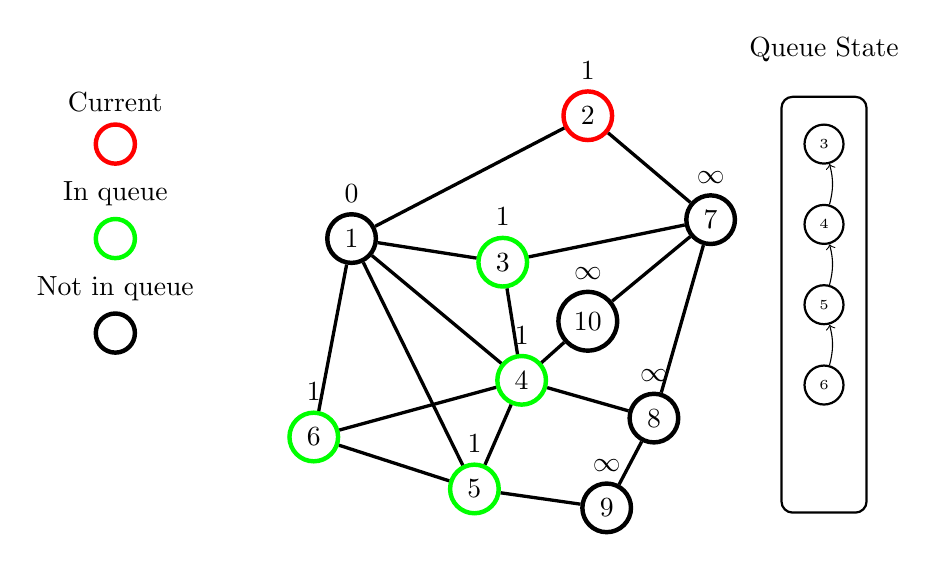
\begin{tikzpicture}[scale=1.2] 
\node[shape=circle, draw=red, 	ultra thick, scale=1.5pt, label={Current}] (U) at (-2.5, 1) {}; 
\node[shape=circle, draw=green,  ultra thick, scale=1.5pt, label={In queue}] (U) at (-2.5, 0) {}; 
\node[shape=circle, draw=black, ultra thick, scale=1.5pt, label={Not in queue}] (U) at (-2.5, -1) {}; 
\draw[thick, rounded corners,draw=black] (4.55, 1.5) rectangle ++(0.9, -1-4*0.85 );
\node[draw=white] at (5, 2) {Queue State} ; 
\node[shape=circle, draw=black, thick, minimum size=2pt] (U0) at (5, 1.0) {\tiny{3}}; 
\node[shape=circle, draw=black, thick, minimum size=2pt] (U1) at (5, 0.15000000000000002) {\tiny{4}}; 
\node[shape=circle, draw=black, thick, minimum size=2pt] (U2) at (5, -0.7) {\tiny{5}}; 
\node[shape=circle, draw=black, thick, minimum size=2pt] (U3) at (5, -1.5499999999999998) {\tiny{6}}; 
\path[->] (U1) edge [out=75, in=-75] (U0);
\path[->] (U2) edge [out=75, in=-75] (U1);
\path[->] (U3) edge [out=75, in=-75] (U2);
\node[shape=circle,draw=black, ultra thick, label={$0$}] (1) at (0,0) {1}; 
\node[shape=circle,draw=red, ultra thick, label={$1$}] (2) at (2.5,1.3) {2}; 
\node[shape=circle,draw=green, ultra thick, label={$1$}] (3) at (1.6,-0.25) {3}; 
\node[shape=circle,draw=green, ultra thick, label={$1$}] (4) at (1.8,-1.5) {4}; 
\node[shape=circle,draw=green, ultra thick, label={$1$}] (5) at (1.3,-2.65) {5}; 
\node[shape=circle,draw=green, ultra thick, label={$1$}] (6) at (-0.4,-2.1) {6}; 
\node[shape=circle,draw=black, ultra thick, label={$\infty$}] (7) at (3.8,0.2) {7}; 
\node[shape=circle,draw=black, ultra thick, label={$\infty$}] (8) at (3.2,-1.9) {8}; 
\node[shape=circle,draw=black, ultra thick, label={$\infty$}] (9) at (2.7,-2.85) {9}; 
\node[shape=circle,draw=black, ultra thick, label={$\infty$}] (10) at (2.5,-0.875) {10}; 
\path [-,very thick, draw=black] (1) edge  (2);
\path [-,very thick, draw=black] (1) edge  (3);
\path [-,very thick, draw=black] (1) edge  (4);
\path [-,very thick, draw=black] (1) edge  (5);
\path [-,very thick, draw=black] (1) edge  (6);
\path [-,very thick, draw=black] (2) edge  (7);
\path [-,very thick, draw=black] (3) edge  (7);
\path [-,very thick, draw=black] (3) edge  (4);
\path [-,very thick, draw=black] (4) edge  (5);
\path [-,very thick, draw=black] (4) edge  (6);
\path [-,very thick, draw=black] (4) edge  (8);
\path [-,very thick, draw=black] (4) edge  (10);
\path [-,very thick, draw=black] (5) edge  (6);
\path [-,very thick, draw=black] (5) edge  (9);
\path [-,very thick, draw=black] (7) edge  (8);
\path [-,very thick, draw=black] (7) edge  (10);
\path [-,very thick, draw=black] (8) edge  (9);
\end{tikzpicture} 
\end{figure} 
\end{frame} 
\begin{frame}{BFS : Example}
\begin{figure}
\vspace*{-1cm} 
\center
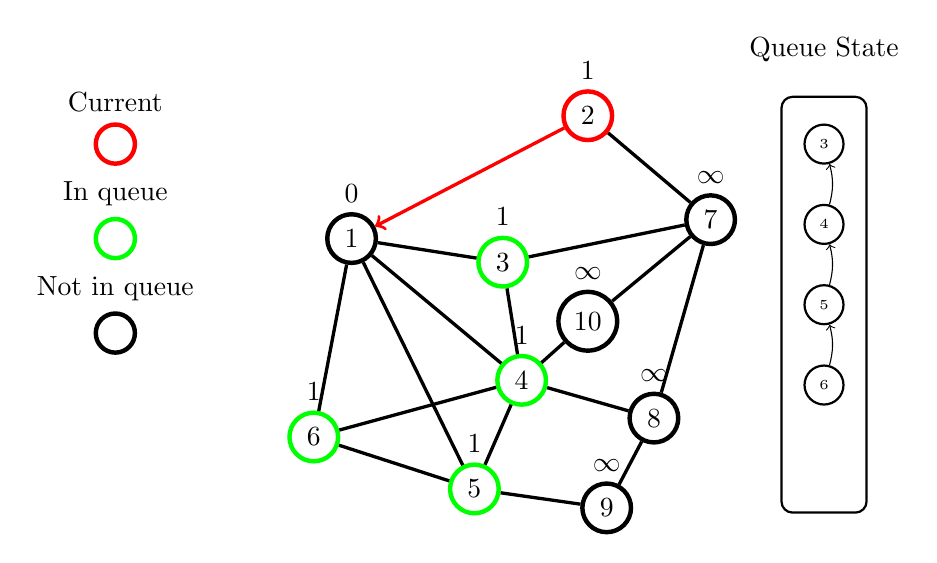
\begin{tikzpicture}[scale=1.2] 
\node[shape=circle, draw=red, 	ultra thick, scale=1.5pt, label={Current}] (U) at (-2.5, 1) {}; 
\node[shape=circle, draw=green,  ultra thick, scale=1.5pt, label={In queue}] (U) at (-2.5, 0) {}; 
\node[shape=circle, draw=black, ultra thick, scale=1.5pt, label={Not in queue}] (U) at (-2.5, -1) {}; 
\draw[thick, rounded corners,draw=black] (4.55, 1.5) rectangle ++(0.9, -1-4*0.85 );
\node[draw=white] at (5, 2) {Queue State} ; 
\node[shape=circle, draw=black, thick, minimum size=2pt] (U0) at (5, 1.0) {\tiny{3}}; 
\node[shape=circle, draw=black, thick, minimum size=2pt] (U1) at (5, 0.15000000000000002) {\tiny{4}}; 
\node[shape=circle, draw=black, thick, minimum size=2pt] (U2) at (5, -0.7) {\tiny{5}}; 
\node[shape=circle, draw=black, thick, minimum size=2pt] (U3) at (5, -1.5499999999999998) {\tiny{6}}; 
\path[->] (U1) edge [out=75, in=-75] (U0);
\path[->] (U2) edge [out=75, in=-75] (U1);
\path[->] (U3) edge [out=75, in=-75] (U2);
\node[shape=circle,draw=black, ultra thick, label={$0$}] (1) at (0,0) {1}; 
\node[shape=circle,draw=red, ultra thick, label={$1$}] (2) at (2.5,1.3) {2}; 
\node[shape=circle,draw=green, ultra thick, label={$1$}] (3) at (1.6,-0.25) {3}; 
\node[shape=circle,draw=green, ultra thick, label={$1$}] (4) at (1.8,-1.5) {4}; 
\node[shape=circle,draw=green, ultra thick, label={$1$}] (5) at (1.3,-2.65) {5}; 
\node[shape=circle,draw=green, ultra thick, label={$1$}] (6) at (-0.4,-2.1) {6}; 
\node[shape=circle,draw=black, ultra thick, label={$\infty$}] (7) at (3.8,0.2) {7}; 
\node[shape=circle,draw=black, ultra thick, label={$\infty$}] (8) at (3.2,-1.9) {8}; 
\node[shape=circle,draw=black, ultra thick, label={$\infty$}] (9) at (2.7,-2.85) {9}; 
\node[shape=circle,draw=black, ultra thick, label={$\infty$}] (10) at (2.5,-0.875) {10}; 
\path [->,very thick, draw=red] (2) edge  (1);
\path [-,very thick, draw=black] (1) edge  (3);
\path [-,very thick, draw=black] (1) edge  (4);
\path [-,very thick, draw=black] (1) edge  (5);
\path [-,very thick, draw=black] (1) edge  (6);
\path [-,very thick, draw=black] (2) edge  (7);
\path [-,very thick, draw=black] (3) edge  (7);
\path [-,very thick, draw=black] (3) edge  (4);
\path [-,very thick, draw=black] (4) edge  (5);
\path [-,very thick, draw=black] (4) edge  (6);
\path [-,very thick, draw=black] (4) edge  (8);
\path [-,very thick, draw=black] (4) edge  (10);
\path [-,very thick, draw=black] (5) edge  (6);
\path [-,very thick, draw=black] (5) edge  (9);
\path [-,very thick, draw=black] (7) edge  (8);
\path [-,very thick, draw=black] (7) edge  (10);
\path [-,very thick, draw=black] (8) edge  (9);
\end{tikzpicture} 
\end{figure} 
\end{frame} 
\begin{frame}{BFS : Example}
\begin{figure}
\vspace*{-1cm} 
\center
\begin{tikzpicture}[scale=1.2] 
\node[shape=circle, draw=red, 	ultra thick, scale=1.5pt, label={Current}] (U) at (-2.5, 1) {}; 
\node[shape=circle, draw=green,  ultra thick, scale=1.5pt, label={In queue}] (U) at (-2.5, 0) {}; 
\node[shape=circle, draw=black, ultra thick, scale=1.5pt, label={Not in queue}] (U) at (-2.5, -1) {}; 
\draw[thick, rounded corners,draw=black] (4.55, 1.5) rectangle ++(0.9, -1-4*0.85 );
\node[draw=white] at (5, 2) {Queue State} ; 
\node[shape=circle, draw=black, thick, minimum size=2pt] (U0) at (5, 1.0) {\tiny{3}}; 
\node[shape=circle, draw=black, thick, minimum size=2pt] (U1) at (5, 0.15000000000000002) {\tiny{4}}; 
\node[shape=circle, draw=black, thick, minimum size=2pt] (U2) at (5, -0.7) {\tiny{5}}; 
\node[shape=circle, draw=black, thick, minimum size=2pt] (U3) at (5, -1.5499999999999998) {\tiny{6}}; 
\node[shape=circle, draw=black, thick, minimum size=2pt] (U4) at (5, -2.4) {\tiny{7}}; 
\path[->] (U1) edge [out=75, in=-75] (U0);
\path[->] (U2) edge [out=75, in=-75] (U1);
\path[->] (U3) edge [out=75, in=-75] (U2);
\path[->] (U4) edge [out=75, in=-75] (U3);
\path[->, thick, draw=black] (7) edge [dashed, bend right=30] (U4); 
\node[shape=circle,draw=black, ultra thick, label={$0$}] (1) at (0,0) {1}; 
\node[shape=circle,draw=red, ultra thick, label={$1$}] (2) at (2.5,1.3) {2}; 
\node[shape=circle,draw=green, ultra thick, label={$1$}] (3) at (1.6,-0.25) {3}; 
\node[shape=circle,draw=green, ultra thick, label={$1$}] (4) at (1.8,-1.5) {4}; 
\node[shape=circle,draw=green, ultra thick, label={$1$}] (5) at (1.3,-2.65) {5}; 
\node[shape=circle,draw=green, ultra thick, label={$1$}] (6) at (-0.4,-2.1) {6}; 
\node[shape=circle,draw=green, ultra thick, label={$2$}] (7) at (3.8,0.2) {7}; 
\node[shape=circle,draw=black, ultra thick, label={$\infty$}] (8) at (3.2,-1.9) {8}; 
\node[shape=circle,draw=black, ultra thick, label={$\infty$}] (9) at (2.7,-2.85) {9}; 
\node[shape=circle,draw=black, ultra thick, label={$\infty$}] (10) at (2.5,-0.875) {10}; 
\path [-,very thick, draw=black] (1) edge  (2);
\path [-,very thick, draw=black] (1) edge  (3);
\path [-,very thick, draw=black] (1) edge  (4);
\path [-,very thick, draw=black] (1) edge  (5);
\path [-,very thick, draw=black] (1) edge  (6);
\path [->,very thick, draw=red] (2) edge  (7);
\path [-,very thick, draw=black] (3) edge  (7);
\path [-,very thick, draw=black] (3) edge  (4);
\path [-,very thick, draw=black] (4) edge  (5);
\path [-,very thick, draw=black] (4) edge  (6);
\path [-,very thick, draw=black] (4) edge  (8);
\path [-,very thick, draw=black] (4) edge  (10);
\path [-,very thick, draw=black] (5) edge  (6);
\path [-,very thick, draw=black] (5) edge  (9);
\path [-,very thick, draw=black] (7) edge  (8);
\path [-,very thick, draw=black] (7) edge  (10);
\path [-,very thick, draw=black] (8) edge  (9);
\end{tikzpicture} 
\end{figure} 
\end{frame} 
\begin{frame}{BFS : Example}
\begin{figure}
\vspace*{-1cm} 
\center
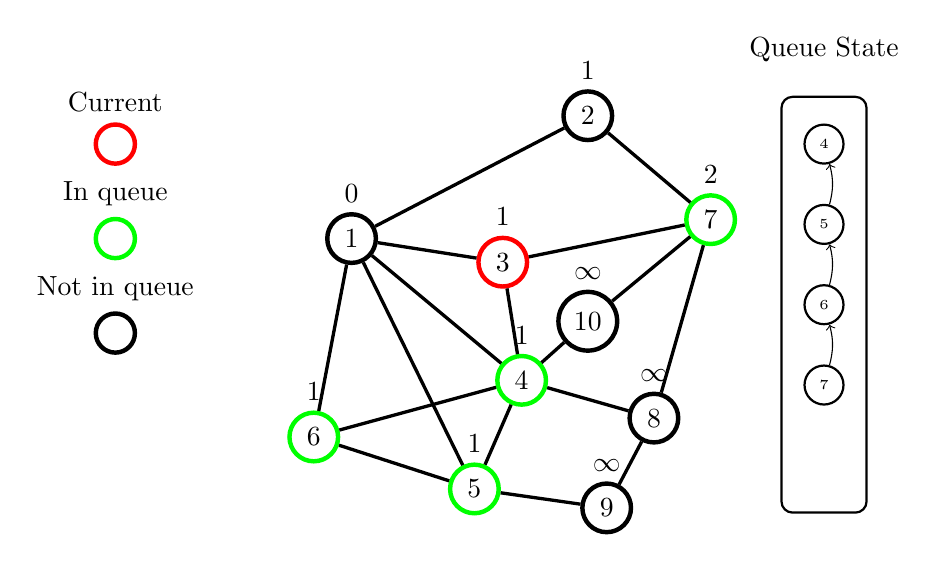
\begin{tikzpicture}[scale=1.2] 
\node[shape=circle, draw=red, 	ultra thick, scale=1.5pt, label={Current}] (U) at (-2.5, 1) {}; 
\node[shape=circle, draw=green,  ultra thick, scale=1.5pt, label={In queue}] (U) at (-2.5, 0) {}; 
\node[shape=circle, draw=black, ultra thick, scale=1.5pt, label={Not in queue}] (U) at (-2.5, -1) {}; 
\draw[thick, rounded corners,draw=black] (4.55, 1.5) rectangle ++(0.9, -1-4*0.85 );
\node[draw=white] at (5, 2) {Queue State} ; 
\node[shape=circle, draw=black, thick, minimum size=2pt] (U0) at (5, 1.0) {\tiny{4}}; 
\node[shape=circle, draw=black, thick, minimum size=2pt] (U1) at (5, 0.15000000000000002) {\tiny{5}}; 
\node[shape=circle, draw=black, thick, minimum size=2pt] (U2) at (5, -0.7) {\tiny{6}}; 
\node[shape=circle, draw=black, thick, minimum size=2pt] (U3) at (5, -1.5499999999999998) {\tiny{7}}; 
\path[->] (U1) edge [out=75, in=-75] (U0);
\path[->] (U2) edge [out=75, in=-75] (U1);
\path[->] (U3) edge [out=75, in=-75] (U2);
\node[shape=circle,draw=black, ultra thick, label={$0$}] (1) at (0,0) {1}; 
\node[shape=circle,draw=black, ultra thick, label={$1$}] (2) at (2.5,1.3) {2}; 
\node[shape=circle,draw=red, ultra thick, label={$1$}] (3) at (1.6,-0.25) {3}; 
\node[shape=circle,draw=green, ultra thick, label={$1$}] (4) at (1.8,-1.5) {4}; 
\node[shape=circle,draw=green, ultra thick, label={$1$}] (5) at (1.3,-2.65) {5}; 
\node[shape=circle,draw=green, ultra thick, label={$1$}] (6) at (-0.4,-2.1) {6}; 
\node[shape=circle,draw=green, ultra thick, label={$2$}] (7) at (3.8,0.2) {7}; 
\node[shape=circle,draw=black, ultra thick, label={$\infty$}] (8) at (3.2,-1.9) {8}; 
\node[shape=circle,draw=black, ultra thick, label={$\infty$}] (9) at (2.7,-2.85) {9}; 
\node[shape=circle,draw=black, ultra thick, label={$\infty$}] (10) at (2.5,-0.875) {10}; 
\path [-,very thick, draw=black] (1) edge  (2);
\path [-,very thick, draw=black] (1) edge  (3);
\path [-,very thick, draw=black] (1) edge  (4);
\path [-,very thick, draw=black] (1) edge  (5);
\path [-,very thick, draw=black] (1) edge  (6);
\path [-,very thick, draw=black] (2) edge  (7);
\path [-,very thick, draw=black] (3) edge  (7);
\path [-,very thick, draw=black] (3) edge  (4);
\path [-,very thick, draw=black] (4) edge  (5);
\path [-,very thick, draw=black] (4) edge  (6);
\path [-,very thick, draw=black] (4) edge  (8);
\path [-,very thick, draw=black] (4) edge  (10);
\path [-,very thick, draw=black] (5) edge  (6);
\path [-,very thick, draw=black] (5) edge  (9);
\path [-,very thick, draw=black] (7) edge  (8);
\path [-,very thick, draw=black] (7) edge  (10);
\path [-,very thick, draw=black] (8) edge  (9);
\end{tikzpicture} 
\end{figure} 
\end{frame} 
\begin{frame}{BFS : Example}
\begin{figure}
\vspace*{-1cm} 
\center
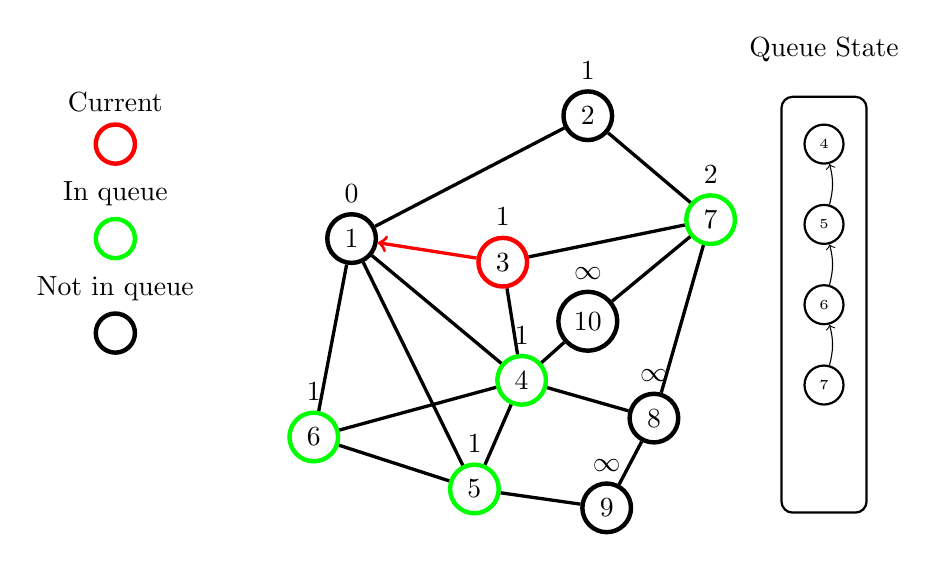
\begin{tikzpicture}[scale=1.2] 
\node[shape=circle, draw=red, 	ultra thick, scale=1.5pt, label={Current}] (U) at (-2.5, 1) {}; 
\node[shape=circle, draw=green,  ultra thick, scale=1.5pt, label={In queue}] (U) at (-2.5, 0) {}; 
\node[shape=circle, draw=black, ultra thick, scale=1.5pt, label={Not in queue}] (U) at (-2.5, -1) {}; 
\draw[thick, rounded corners,draw=black] (4.55, 1.5) rectangle ++(0.9, -1-4*0.85 );
\node[draw=white] at (5, 2) {Queue State} ; 
\node[shape=circle, draw=black, thick, minimum size=2pt] (U0) at (5, 1.0) {\tiny{4}}; 
\node[shape=circle, draw=black, thick, minimum size=2pt] (U1) at (5, 0.15000000000000002) {\tiny{5}}; 
\node[shape=circle, draw=black, thick, minimum size=2pt] (U2) at (5, -0.7) {\tiny{6}}; 
\node[shape=circle, draw=black, thick, minimum size=2pt] (U3) at (5, -1.5499999999999998) {\tiny{7}}; 
\path[->] (U1) edge [out=75, in=-75] (U0);
\path[->] (U2) edge [out=75, in=-75] (U1);
\path[->] (U3) edge [out=75, in=-75] (U2);
\node[shape=circle,draw=black, ultra thick, label={$0$}] (1) at (0,0) {1}; 
\node[shape=circle,draw=black, ultra thick, label={$1$}] (2) at (2.5,1.3) {2}; 
\node[shape=circle,draw=red, ultra thick, label={$1$}] (3) at (1.6,-0.25) {3}; 
\node[shape=circle,draw=green, ultra thick, label={$1$}] (4) at (1.8,-1.5) {4}; 
\node[shape=circle,draw=green, ultra thick, label={$1$}] (5) at (1.3,-2.65) {5}; 
\node[shape=circle,draw=green, ultra thick, label={$1$}] (6) at (-0.4,-2.1) {6}; 
\node[shape=circle,draw=green, ultra thick, label={$2$}] (7) at (3.8,0.2) {7}; 
\node[shape=circle,draw=black, ultra thick, label={$\infty$}] (8) at (3.2,-1.9) {8}; 
\node[shape=circle,draw=black, ultra thick, label={$\infty$}] (9) at (2.7,-2.85) {9}; 
\node[shape=circle,draw=black, ultra thick, label={$\infty$}] (10) at (2.5,-0.875) {10}; 
\path [-,very thick, draw=black] (1) edge  (2);
\path [->,very thick, draw=red] (3) edge  (1);
\path [-,very thick, draw=black] (1) edge  (4);
\path [-,very thick, draw=black] (1) edge  (5);
\path [-,very thick, draw=black] (1) edge  (6);
\path [-,very thick, draw=black] (2) edge  (7);
\path [-,very thick, draw=black] (3) edge  (7);
\path [-,very thick, draw=black] (3) edge  (4);
\path [-,very thick, draw=black] (4) edge  (5);
\path [-,very thick, draw=black] (4) edge  (6);
\path [-,very thick, draw=black] (4) edge  (8);
\path [-,very thick, draw=black] (4) edge  (10);
\path [-,very thick, draw=black] (5) edge  (6);
\path [-,very thick, draw=black] (5) edge  (9);
\path [-,very thick, draw=black] (7) edge  (8);
\path [-,very thick, draw=black] (7) edge  (10);
\path [-,very thick, draw=black] (8) edge  (9);
\end{tikzpicture} 
\end{figure} 
\end{frame} 
\begin{frame}{BFS : Example}
\begin{figure}
\vspace*{-1cm} 
\center
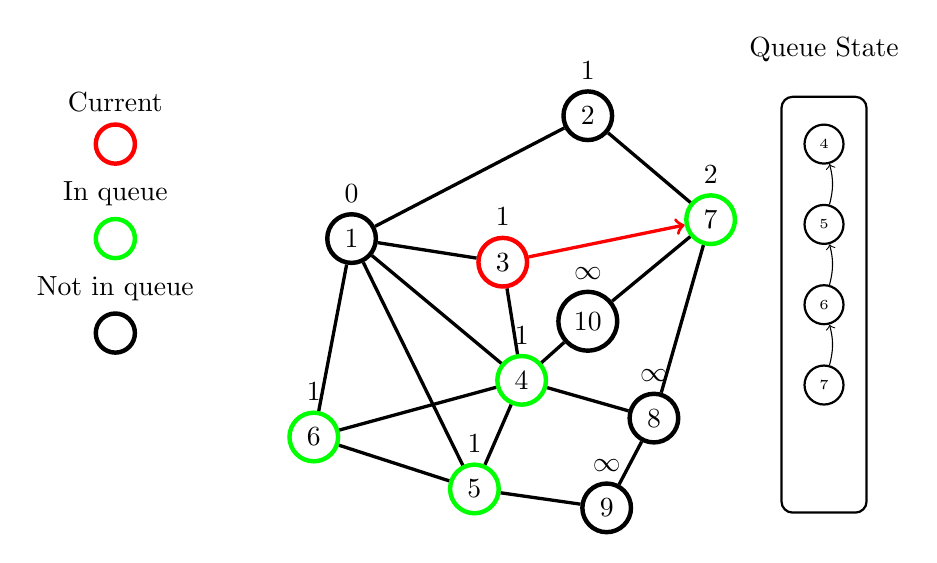
\begin{tikzpicture}[scale=1.2] 
\node[shape=circle, draw=red, 	ultra thick, scale=1.5pt, label={Current}] (U) at (-2.5, 1) {}; 
\node[shape=circle, draw=green,  ultra thick, scale=1.5pt, label={In queue}] (U) at (-2.5, 0) {}; 
\node[shape=circle, draw=black, ultra thick, scale=1.5pt, label={Not in queue}] (U) at (-2.5, -1) {}; 
\draw[thick, rounded corners,draw=black] (4.55, 1.5) rectangle ++(0.9, -1-4*0.85 );
\node[draw=white] at (5, 2) {Queue State} ; 
\node[shape=circle, draw=black, thick, minimum size=2pt] (U0) at (5, 1.0) {\tiny{4}}; 
\node[shape=circle, draw=black, thick, minimum size=2pt] (U1) at (5, 0.15000000000000002) {\tiny{5}}; 
\node[shape=circle, draw=black, thick, minimum size=2pt] (U2) at (5, -0.7) {\tiny{6}}; 
\node[shape=circle, draw=black, thick, minimum size=2pt] (U3) at (5, -1.5499999999999998) {\tiny{7}}; 
\path[->] (U1) edge [out=75, in=-75] (U0);
\path[->] (U2) edge [out=75, in=-75] (U1);
\path[->] (U3) edge [out=75, in=-75] (U2);
\node[shape=circle,draw=black, ultra thick, label={$0$}] (1) at (0,0) {1}; 
\node[shape=circle,draw=black, ultra thick, label={$1$}] (2) at (2.5,1.3) {2}; 
\node[shape=circle,draw=red, ultra thick, label={$1$}] (3) at (1.6,-0.25) {3}; 
\node[shape=circle,draw=green, ultra thick, label={$1$}] (4) at (1.8,-1.5) {4}; 
\node[shape=circle,draw=green, ultra thick, label={$1$}] (5) at (1.3,-2.65) {5}; 
\node[shape=circle,draw=green, ultra thick, label={$1$}] (6) at (-0.4,-2.1) {6}; 
\node[shape=circle,draw=green, ultra thick, label={$2$}] (7) at (3.8,0.2) {7}; 
\node[shape=circle,draw=black, ultra thick, label={$\infty$}] (8) at (3.2,-1.9) {8}; 
\node[shape=circle,draw=black, ultra thick, label={$\infty$}] (9) at (2.7,-2.85) {9}; 
\node[shape=circle,draw=black, ultra thick, label={$\infty$}] (10) at (2.5,-0.875) {10}; 
\path [-,very thick, draw=black] (1) edge  (2);
\path [-,very thick, draw=black] (1) edge  (3);
\path [-,very thick, draw=black] (1) edge  (4);
\path [-,very thick, draw=black] (1) edge  (5);
\path [-,very thick, draw=black] (1) edge  (6);
\path [-,very thick, draw=black] (2) edge  (7);
\path [->,very thick, draw=red] (3) edge  (7);
\path [-,very thick, draw=black] (3) edge  (4);
\path [-,very thick, draw=black] (4) edge  (5);
\path [-,very thick, draw=black] (4) edge  (6);
\path [-,very thick, draw=black] (4) edge  (8);
\path [-,very thick, draw=black] (4) edge  (10);
\path [-,very thick, draw=black] (5) edge  (6);
\path [-,very thick, draw=black] (5) edge  (9);
\path [-,very thick, draw=black] (7) edge  (8);
\path [-,very thick, draw=black] (7) edge  (10);
\path [-,very thick, draw=black] (8) edge  (9);
\end{tikzpicture} 
\end{figure} 
\end{frame} 
\begin{frame}{BFS : Example}
\begin{figure}
\vspace*{-1cm} 
\center
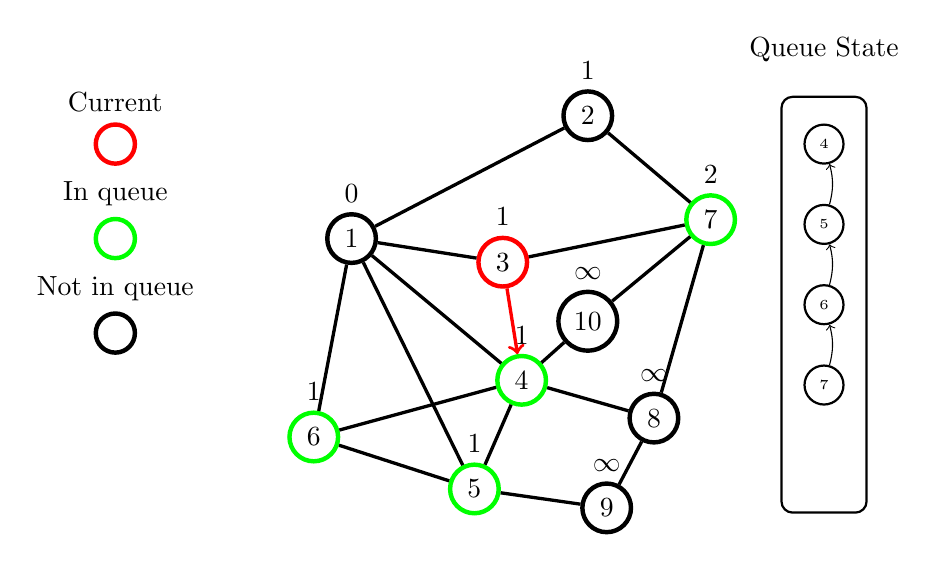
\begin{tikzpicture}[scale=1.2] 
\node[shape=circle, draw=red, 	ultra thick, scale=1.5pt, label={Current}] (U) at (-2.5, 1) {}; 
\node[shape=circle, draw=green,  ultra thick, scale=1.5pt, label={In queue}] (U) at (-2.5, 0) {}; 
\node[shape=circle, draw=black, ultra thick, scale=1.5pt, label={Not in queue}] (U) at (-2.5, -1) {}; 
\draw[thick, rounded corners,draw=black] (4.55, 1.5) rectangle ++(0.9, -1-4*0.85 );
\node[draw=white] at (5, 2) {Queue State} ; 
\node[shape=circle, draw=black, thick, minimum size=2pt] (U0) at (5, 1.0) {\tiny{4}}; 
\node[shape=circle, draw=black, thick, minimum size=2pt] (U1) at (5, 0.15000000000000002) {\tiny{5}}; 
\node[shape=circle, draw=black, thick, minimum size=2pt] (U2) at (5, -0.7) {\tiny{6}}; 
\node[shape=circle, draw=black, thick, minimum size=2pt] (U3) at (5, -1.5499999999999998) {\tiny{7}}; 
\path[->] (U1) edge [out=75, in=-75] (U0);
\path[->] (U2) edge [out=75, in=-75] (U1);
\path[->] (U3) edge [out=75, in=-75] (U2);
\node[shape=circle,draw=black, ultra thick, label={$0$}] (1) at (0,0) {1}; 
\node[shape=circle,draw=black, ultra thick, label={$1$}] (2) at (2.5,1.3) {2}; 
\node[shape=circle,draw=red, ultra thick, label={$1$}] (3) at (1.6,-0.25) {3}; 
\node[shape=circle,draw=green, ultra thick, label={$1$}] (4) at (1.8,-1.5) {4}; 
\node[shape=circle,draw=green, ultra thick, label={$1$}] (5) at (1.3,-2.65) {5}; 
\node[shape=circle,draw=green, ultra thick, label={$1$}] (6) at (-0.4,-2.1) {6}; 
\node[shape=circle,draw=green, ultra thick, label={$2$}] (7) at (3.8,0.2) {7}; 
\node[shape=circle,draw=black, ultra thick, label={$\infty$}] (8) at (3.2,-1.9) {8}; 
\node[shape=circle,draw=black, ultra thick, label={$\infty$}] (9) at (2.7,-2.85) {9}; 
\node[shape=circle,draw=black, ultra thick, label={$\infty$}] (10) at (2.5,-0.875) {10}; 
\path [-,very thick, draw=black] (1) edge  (2);
\path [-,very thick, draw=black] (1) edge  (3);
\path [-,very thick, draw=black] (1) edge  (4);
\path [-,very thick, draw=black] (1) edge  (5);
\path [-,very thick, draw=black] (1) edge  (6);
\path [-,very thick, draw=black] (2) edge  (7);
\path [-,very thick, draw=black] (3) edge  (7);
\path [->,very thick, draw=red] (3) edge  (4);
\path [-,very thick, draw=black] (4) edge  (5);
\path [-,very thick, draw=black] (4) edge  (6);
\path [-,very thick, draw=black] (4) edge  (8);
\path [-,very thick, draw=black] (4) edge  (10);
\path [-,very thick, draw=black] (5) edge  (6);
\path [-,very thick, draw=black] (5) edge  (9);
\path [-,very thick, draw=black] (7) edge  (8);
\path [-,very thick, draw=black] (7) edge  (10);
\path [-,very thick, draw=black] (8) edge  (9);
\end{tikzpicture} 
\end{figure} 
\end{frame} 
\begin{frame}{BFS : Example}
\begin{figure}
\vspace*{-1cm} 
\center
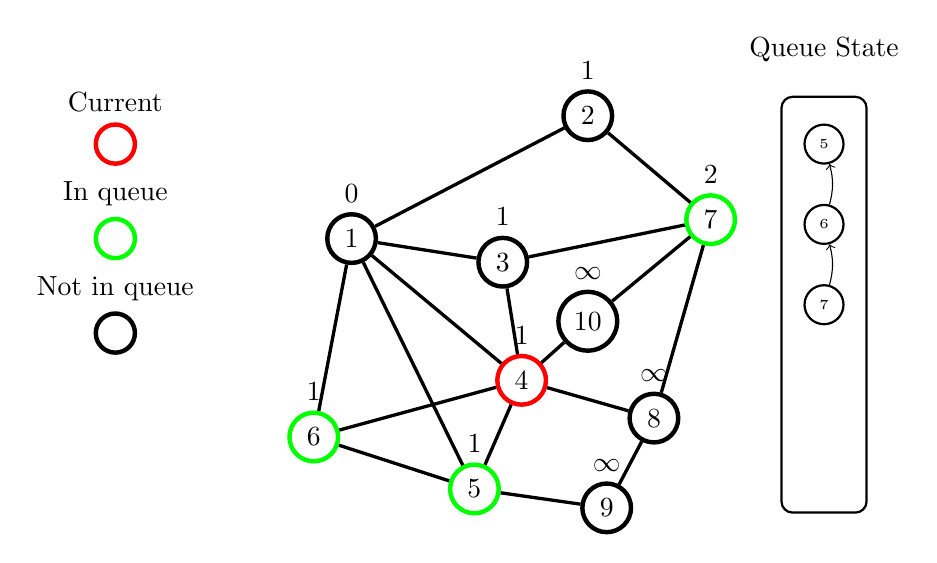
\begin{tikzpicture}[scale=1.2] 
\node[shape=circle, draw=red, 	ultra thick, scale=1.5pt, label={Current}] (U) at (-2.5, 1) {}; 
\node[shape=circle, draw=green,  ultra thick, scale=1.5pt, label={In queue}] (U) at (-2.5, 0) {}; 
\node[shape=circle, draw=black, ultra thick, scale=1.5pt, label={Not in queue}] (U) at (-2.5, -1) {}; 
\draw[thick, rounded corners,draw=black] (4.55, 1.5) rectangle ++(0.9, -1-4*0.85 );
\node[draw=white] at (5, 2) {Queue State} ; 
\node[shape=circle, draw=black, thick, minimum size=2pt] (U0) at (5, 1.0) {\tiny{5}}; 
\node[shape=circle, draw=black, thick, minimum size=2pt] (U1) at (5, 0.15000000000000002) {\tiny{6}}; 
\node[shape=circle, draw=black, thick, minimum size=2pt] (U2) at (5, -0.7) {\tiny{7}}; 
\path[->] (U1) edge [out=75, in=-75] (U0);
\path[->] (U2) edge [out=75, in=-75] (U1);
\node[shape=circle,draw=black, ultra thick, label={$0$}] (1) at (0,0) {1}; 
\node[shape=circle,draw=black, ultra thick, label={$1$}] (2) at (2.5,1.3) {2}; 
\node[shape=circle,draw=black, ultra thick, label={$1$}] (3) at (1.6,-0.25) {3}; 
\node[shape=circle,draw=red, ultra thick, label={$1$}] (4) at (1.8,-1.5) {4}; 
\node[shape=circle,draw=green, ultra thick, label={$1$}] (5) at (1.3,-2.65) {5}; 
\node[shape=circle,draw=green, ultra thick, label={$1$}] (6) at (-0.4,-2.1) {6}; 
\node[shape=circle,draw=green, ultra thick, label={$2$}] (7) at (3.8,0.2) {7}; 
\node[shape=circle,draw=black, ultra thick, label={$\infty$}] (8) at (3.2,-1.9) {8}; 
\node[shape=circle,draw=black, ultra thick, label={$\infty$}] (9) at (2.7,-2.85) {9}; 
\node[shape=circle,draw=black, ultra thick, label={$\infty$}] (10) at (2.5,-0.875) {10}; 
\path [-,very thick, draw=black] (1) edge  (2);
\path [-,very thick, draw=black] (1) edge  (3);
\path [-,very thick, draw=black] (1) edge  (4);
\path [-,very thick, draw=black] (1) edge  (5);
\path [-,very thick, draw=black] (1) edge  (6);
\path [-,very thick, draw=black] (2) edge  (7);
\path [-,very thick, draw=black] (3) edge  (7);
\path [-,very thick, draw=black] (3) edge  (4);
\path [-,very thick, draw=black] (4) edge  (5);
\path [-,very thick, draw=black] (4) edge  (6);
\path [-,very thick, draw=black] (4) edge  (8);
\path [-,very thick, draw=black] (4) edge  (10);
\path [-,very thick, draw=black] (5) edge  (6);
\path [-,very thick, draw=black] (5) edge  (9);
\path [-,very thick, draw=black] (7) edge  (8);
\path [-,very thick, draw=black] (7) edge  (10);
\path [-,very thick, draw=black] (8) edge  (9);
\end{tikzpicture} 
\end{figure} 
\end{frame} 
\begin{frame}{BFS : Example}
\begin{figure}
\vspace*{-1cm} 
\center
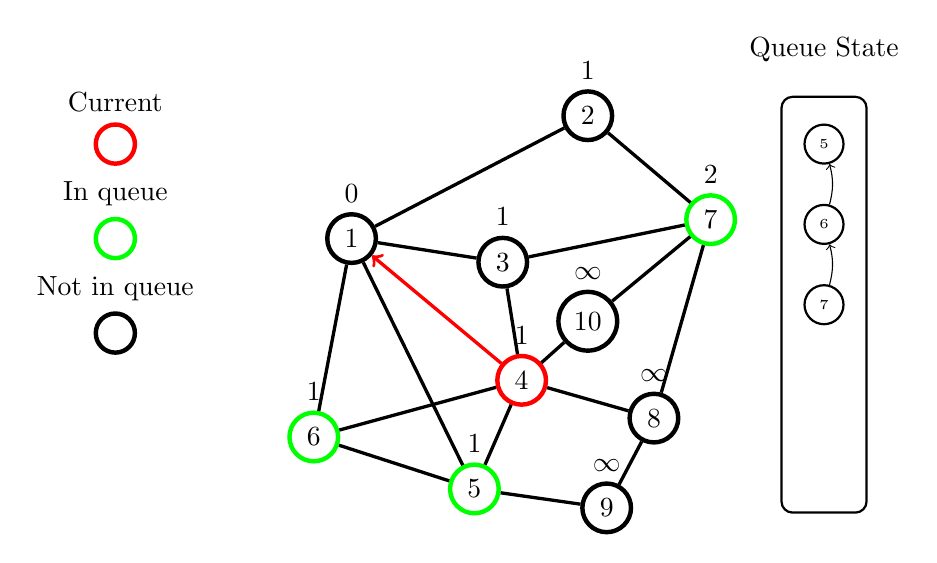
\begin{tikzpicture}[scale=1.2] 
\node[shape=circle, draw=red, 	ultra thick, scale=1.5pt, label={Current}] (U) at (-2.5, 1) {}; 
\node[shape=circle, draw=green,  ultra thick, scale=1.5pt, label={In queue}] (U) at (-2.5, 0) {}; 
\node[shape=circle, draw=black, ultra thick, scale=1.5pt, label={Not in queue}] (U) at (-2.5, -1) {}; 
\draw[thick, rounded corners,draw=black] (4.55, 1.5) rectangle ++(0.9, -1-4*0.85 );
\node[draw=white] at (5, 2) {Queue State} ; 
\node[shape=circle, draw=black, thick, minimum size=2pt] (U0) at (5, 1.0) {\tiny{5}}; 
\node[shape=circle, draw=black, thick, minimum size=2pt] (U1) at (5, 0.15000000000000002) {\tiny{6}}; 
\node[shape=circle, draw=black, thick, minimum size=2pt] (U2) at (5, -0.7) {\tiny{7}}; 
\path[->] (U1) edge [out=75, in=-75] (U0);
\path[->] (U2) edge [out=75, in=-75] (U1);
\node[shape=circle,draw=black, ultra thick, label={$0$}] (1) at (0,0) {1}; 
\node[shape=circle,draw=black, ultra thick, label={$1$}] (2) at (2.5,1.3) {2}; 
\node[shape=circle,draw=black, ultra thick, label={$1$}] (3) at (1.6,-0.25) {3}; 
\node[shape=circle,draw=red, ultra thick, label={$1$}] (4) at (1.8,-1.5) {4}; 
\node[shape=circle,draw=green, ultra thick, label={$1$}] (5) at (1.3,-2.65) {5}; 
\node[shape=circle,draw=green, ultra thick, label={$1$}] (6) at (-0.4,-2.1) {6}; 
\node[shape=circle,draw=green, ultra thick, label={$2$}] (7) at (3.8,0.2) {7}; 
\node[shape=circle,draw=black, ultra thick, label={$\infty$}] (8) at (3.2,-1.9) {8}; 
\node[shape=circle,draw=black, ultra thick, label={$\infty$}] (9) at (2.7,-2.85) {9}; 
\node[shape=circle,draw=black, ultra thick, label={$\infty$}] (10) at (2.5,-0.875) {10}; 
\path [-,very thick, draw=black] (1) edge  (2);
\path [-,very thick, draw=black] (1) edge  (3);
\path [->,very thick, draw=red] (4) edge  (1);
\path [-,very thick, draw=black] (1) edge  (5);
\path [-,very thick, draw=black] (1) edge  (6);
\path [-,very thick, draw=black] (2) edge  (7);
\path [-,very thick, draw=black] (3) edge  (7);
\path [-,very thick, draw=black] (3) edge  (4);
\path [-,very thick, draw=black] (4) edge  (5);
\path [-,very thick, draw=black] (4) edge  (6);
\path [-,very thick, draw=black] (4) edge  (8);
\path [-,very thick, draw=black] (4) edge  (10);
\path [-,very thick, draw=black] (5) edge  (6);
\path [-,very thick, draw=black] (5) edge  (9);
\path [-,very thick, draw=black] (7) edge  (8);
\path [-,very thick, draw=black] (7) edge  (10);
\path [-,very thick, draw=black] (8) edge  (9);
\end{tikzpicture} 
\end{figure} 
\end{frame} 
\begin{frame}{BFS : Example}
\begin{figure}
\vspace*{-1cm} 
\center
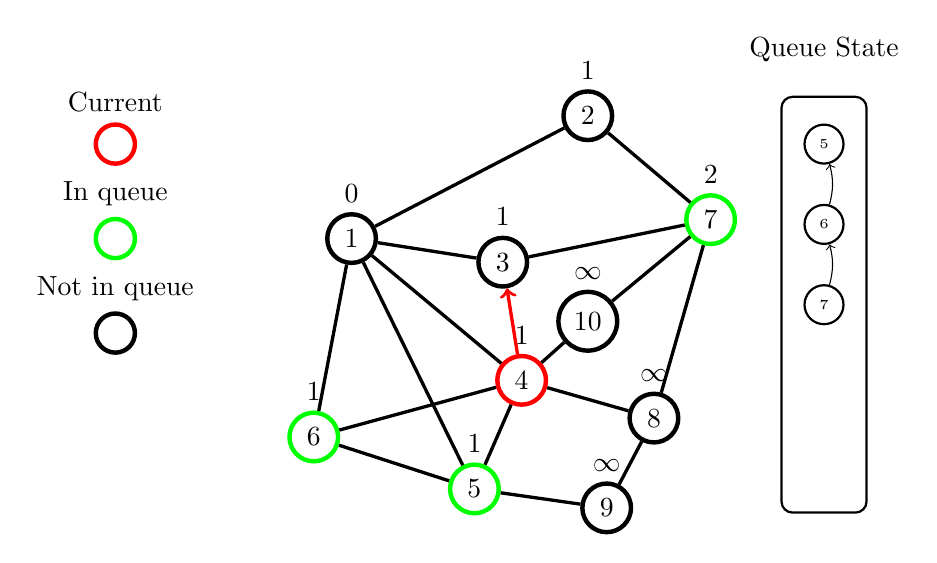
\begin{tikzpicture}[scale=1.2] 
\node[shape=circle, draw=red, 	ultra thick, scale=1.5pt, label={Current}] (U) at (-2.5, 1) {}; 
\node[shape=circle, draw=green,  ultra thick, scale=1.5pt, label={In queue}] (U) at (-2.5, 0) {}; 
\node[shape=circle, draw=black, ultra thick, scale=1.5pt, label={Not in queue}] (U) at (-2.5, -1) {}; 
\draw[thick, rounded corners,draw=black] (4.55, 1.5) rectangle ++(0.9, -1-4*0.85 );
\node[draw=white] at (5, 2) {Queue State} ; 
\node[shape=circle, draw=black, thick, minimum size=2pt] (U0) at (5, 1.0) {\tiny{5}}; 
\node[shape=circle, draw=black, thick, minimum size=2pt] (U1) at (5, 0.15000000000000002) {\tiny{6}}; 
\node[shape=circle, draw=black, thick, minimum size=2pt] (U2) at (5, -0.7) {\tiny{7}}; 
\path[->] (U1) edge [out=75, in=-75] (U0);
\path[->] (U2) edge [out=75, in=-75] (U1);
\node[shape=circle,draw=black, ultra thick, label={$0$}] (1) at (0,0) {1}; 
\node[shape=circle,draw=black, ultra thick, label={$1$}] (2) at (2.5,1.3) {2}; 
\node[shape=circle,draw=black, ultra thick, label={$1$}] (3) at (1.6,-0.25) {3}; 
\node[shape=circle,draw=red, ultra thick, label={$1$}] (4) at (1.8,-1.5) {4}; 
\node[shape=circle,draw=green, ultra thick, label={$1$}] (5) at (1.3,-2.65) {5}; 
\node[shape=circle,draw=green, ultra thick, label={$1$}] (6) at (-0.4,-2.1) {6}; 
\node[shape=circle,draw=green, ultra thick, label={$2$}] (7) at (3.8,0.2) {7}; 
\node[shape=circle,draw=black, ultra thick, label={$\infty$}] (8) at (3.2,-1.9) {8}; 
\node[shape=circle,draw=black, ultra thick, label={$\infty$}] (9) at (2.7,-2.85) {9}; 
\node[shape=circle,draw=black, ultra thick, label={$\infty$}] (10) at (2.5,-0.875) {10}; 
\path [-,very thick, draw=black] (1) edge  (2);
\path [-,very thick, draw=black] (1) edge  (3);
\path [-,very thick, draw=black] (1) edge  (4);
\path [-,very thick, draw=black] (1) edge  (5);
\path [-,very thick, draw=black] (1) edge  (6);
\path [-,very thick, draw=black] (2) edge  (7);
\path [-,very thick, draw=black] (3) edge  (7);
\path [->,very thick, draw=red] (4) edge  (3);
\path [-,very thick, draw=black] (4) edge  (5);
\path [-,very thick, draw=black] (4) edge  (6);
\path [-,very thick, draw=black] (4) edge  (8);
\path [-,very thick, draw=black] (4) edge  (10);
\path [-,very thick, draw=black] (5) edge  (6);
\path [-,very thick, draw=black] (5) edge  (9);
\path [-,very thick, draw=black] (7) edge  (8);
\path [-,very thick, draw=black] (7) edge  (10);
\path [-,very thick, draw=black] (8) edge  (9);
\end{tikzpicture} 
\end{figure} 
\end{frame} 
\begin{frame}{BFS : Example}
\begin{figure}
\vspace*{-1cm} 
\center
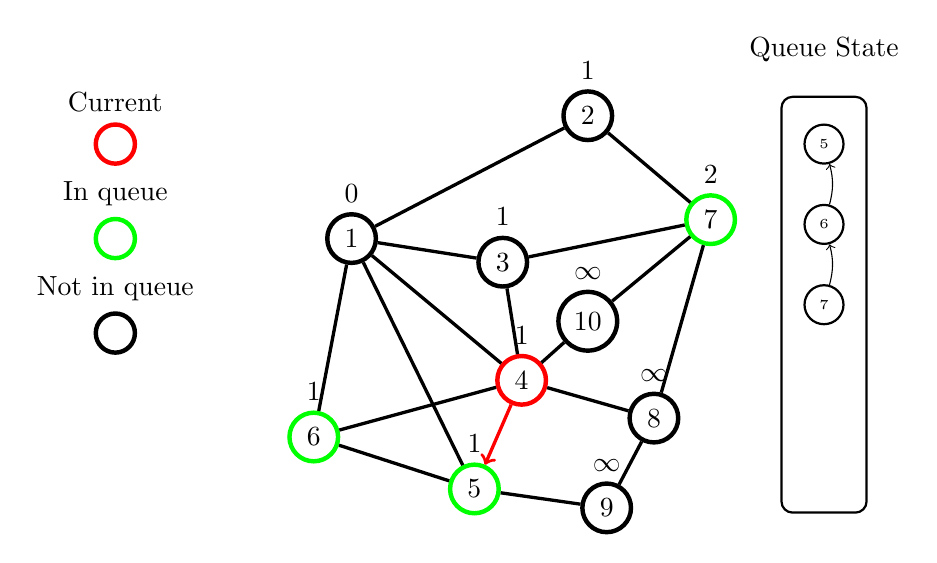
\begin{tikzpicture}[scale=1.2] 
\node[shape=circle, draw=red, 	ultra thick, scale=1.5pt, label={Current}] (U) at (-2.5, 1) {}; 
\node[shape=circle, draw=green,  ultra thick, scale=1.5pt, label={In queue}] (U) at (-2.5, 0) {}; 
\node[shape=circle, draw=black, ultra thick, scale=1.5pt, label={Not in queue}] (U) at (-2.5, -1) {}; 
\draw[thick, rounded corners,draw=black] (4.55, 1.5) rectangle ++(0.9, -1-4*0.85 );
\node[draw=white] at (5, 2) {Queue State} ; 
\node[shape=circle, draw=black, thick, minimum size=2pt] (U0) at (5, 1.0) {\tiny{5}}; 
\node[shape=circle, draw=black, thick, minimum size=2pt] (U1) at (5, 0.15000000000000002) {\tiny{6}}; 
\node[shape=circle, draw=black, thick, minimum size=2pt] (U2) at (5, -0.7) {\tiny{7}}; 
\path[->] (U1) edge [out=75, in=-75] (U0);
\path[->] (U2) edge [out=75, in=-75] (U1);
\node[shape=circle,draw=black, ultra thick, label={$0$}] (1) at (0,0) {1}; 
\node[shape=circle,draw=black, ultra thick, label={$1$}] (2) at (2.5,1.3) {2}; 
\node[shape=circle,draw=black, ultra thick, label={$1$}] (3) at (1.6,-0.25) {3}; 
\node[shape=circle,draw=red, ultra thick, label={$1$}] (4) at (1.8,-1.5) {4}; 
\node[shape=circle,draw=green, ultra thick, label={$1$}] (5) at (1.3,-2.65) {5}; 
\node[shape=circle,draw=green, ultra thick, label={$1$}] (6) at (-0.4,-2.1) {6}; 
\node[shape=circle,draw=green, ultra thick, label={$2$}] (7) at (3.8,0.2) {7}; 
\node[shape=circle,draw=black, ultra thick, label={$\infty$}] (8) at (3.2,-1.9) {8}; 
\node[shape=circle,draw=black, ultra thick, label={$\infty$}] (9) at (2.7,-2.85) {9}; 
\node[shape=circle,draw=black, ultra thick, label={$\infty$}] (10) at (2.5,-0.875) {10}; 
\path [-,very thick, draw=black] (1) edge  (2);
\path [-,very thick, draw=black] (1) edge  (3);
\path [-,very thick, draw=black] (1) edge  (4);
\path [-,very thick, draw=black] (1) edge  (5);
\path [-,very thick, draw=black] (1) edge  (6);
\path [-,very thick, draw=black] (2) edge  (7);
\path [-,very thick, draw=black] (3) edge  (7);
\path [-,very thick, draw=black] (3) edge  (4);
\path [->,very thick, draw=red] (4) edge  (5);
\path [-,very thick, draw=black] (4) edge  (6);
\path [-,very thick, draw=black] (4) edge  (8);
\path [-,very thick, draw=black] (4) edge  (10);
\path [-,very thick, draw=black] (5) edge  (6);
\path [-,very thick, draw=black] (5) edge  (9);
\path [-,very thick, draw=black] (7) edge  (8);
\path [-,very thick, draw=black] (7) edge  (10);
\path [-,very thick, draw=black] (8) edge  (9);
\end{tikzpicture} 
\end{figure} 
\end{frame} 
\begin{frame}{BFS : Example}
\begin{figure}
\vspace*{-1cm} 
\center
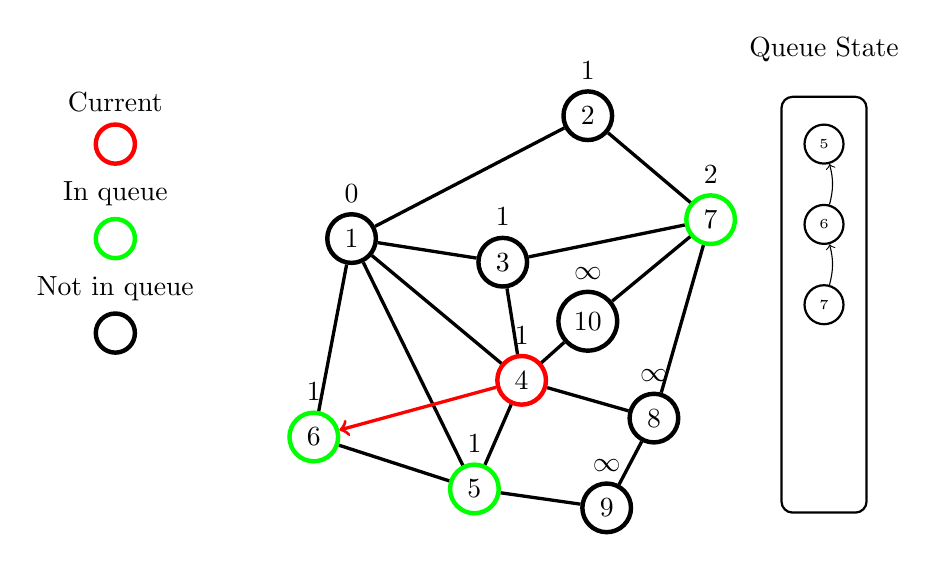
\begin{tikzpicture}[scale=1.2] 
\node[shape=circle, draw=red, 	ultra thick, scale=1.5pt, label={Current}] (U) at (-2.5, 1) {}; 
\node[shape=circle, draw=green,  ultra thick, scale=1.5pt, label={In queue}] (U) at (-2.5, 0) {}; 
\node[shape=circle, draw=black, ultra thick, scale=1.5pt, label={Not in queue}] (U) at (-2.5, -1) {}; 
\draw[thick, rounded corners,draw=black] (4.55, 1.5) rectangle ++(0.9, -1-4*0.85 );
\node[draw=white] at (5, 2) {Queue State} ; 
\node[shape=circle, draw=black, thick, minimum size=2pt] (U0) at (5, 1.0) {\tiny{5}}; 
\node[shape=circle, draw=black, thick, minimum size=2pt] (U1) at (5, 0.15000000000000002) {\tiny{6}}; 
\node[shape=circle, draw=black, thick, minimum size=2pt] (U2) at (5, -0.7) {\tiny{7}}; 
\path[->] (U1) edge [out=75, in=-75] (U0);
\path[->] (U2) edge [out=75, in=-75] (U1);
\node[shape=circle,draw=black, ultra thick, label={$0$}] (1) at (0,0) {1}; 
\node[shape=circle,draw=black, ultra thick, label={$1$}] (2) at (2.5,1.3) {2}; 
\node[shape=circle,draw=black, ultra thick, label={$1$}] (3) at (1.6,-0.25) {3}; 
\node[shape=circle,draw=red, ultra thick, label={$1$}] (4) at (1.8,-1.5) {4}; 
\node[shape=circle,draw=green, ultra thick, label={$1$}] (5) at (1.3,-2.65) {5}; 
\node[shape=circle,draw=green, ultra thick, label={$1$}] (6) at (-0.4,-2.1) {6}; 
\node[shape=circle,draw=green, ultra thick, label={$2$}] (7) at (3.8,0.2) {7}; 
\node[shape=circle,draw=black, ultra thick, label={$\infty$}] (8) at (3.2,-1.9) {8}; 
\node[shape=circle,draw=black, ultra thick, label={$\infty$}] (9) at (2.7,-2.85) {9}; 
\node[shape=circle,draw=black, ultra thick, label={$\infty$}] (10) at (2.5,-0.875) {10}; 
\path [-,very thick, draw=black] (1) edge  (2);
\path [-,very thick, draw=black] (1) edge  (3);
\path [-,very thick, draw=black] (1) edge  (4);
\path [-,very thick, draw=black] (1) edge  (5);
\path [-,very thick, draw=black] (1) edge  (6);
\path [-,very thick, draw=black] (2) edge  (7);
\path [-,very thick, draw=black] (3) edge  (7);
\path [-,very thick, draw=black] (3) edge  (4);
\path [-,very thick, draw=black] (4) edge  (5);
\path [->,very thick, draw=red] (4) edge  (6);
\path [-,very thick, draw=black] (4) edge  (8);
\path [-,very thick, draw=black] (4) edge  (10);
\path [-,very thick, draw=black] (5) edge  (6);
\path [-,very thick, draw=black] (5) edge  (9);
\path [-,very thick, draw=black] (7) edge  (8);
\path [-,very thick, draw=black] (7) edge  (10);
\path [-,very thick, draw=black] (8) edge  (9);
\end{tikzpicture} 
\end{figure} 
\end{frame} 
\begin{frame}{BFS : Example}
\begin{figure}
\vspace*{-1cm} 
\center
\begin{tikzpicture}[scale=1.2] 
\node[shape=circle, draw=red, 	ultra thick, scale=1.5pt, label={Current}] (U) at (-2.5, 1) {}; 
\node[shape=circle, draw=green,  ultra thick, scale=1.5pt, label={In queue}] (U) at (-2.5, 0) {}; 
\node[shape=circle, draw=black, ultra thick, scale=1.5pt, label={Not in queue}] (U) at (-2.5, -1) {}; 
\draw[thick, rounded corners,draw=black] (4.55, 1.5) rectangle ++(0.9, -1-4*0.85 );
\node[draw=white] at (5, 2) {Queue State} ; 
\node[shape=circle, draw=black, thick, minimum size=2pt] (U0) at (5, 1.0) {\tiny{5}}; 
\node[shape=circle, draw=black, thick, minimum size=2pt] (U1) at (5, 0.15000000000000002) {\tiny{6}}; 
\node[shape=circle, draw=black, thick, minimum size=2pt] (U2) at (5, -0.7) {\tiny{7}}; 
\node[shape=circle, draw=black, thick, minimum size=2pt] (U3) at (5, -1.5499999999999998) {\tiny{8}}; 
\path[->] (U1) edge [out=75, in=-75] (U0);
\path[->] (U2) edge [out=75, in=-75] (U1);
\path[->] (U3) edge [out=75, in=-75] (U2);
\path[->, thick, draw=black] (8) edge [dashed, bend right=30] (U3); 
\node[shape=circle,draw=black, ultra thick, label={$0$}] (1) at (0,0) {1}; 
\node[shape=circle,draw=black, ultra thick, label={$1$}] (2) at (2.5,1.3) {2}; 
\node[shape=circle,draw=black, ultra thick, label={$1$}] (3) at (1.6,-0.25) {3}; 
\node[shape=circle,draw=red, ultra thick, label={$1$}] (4) at (1.8,-1.5) {4}; 
\node[shape=circle,draw=green, ultra thick, label={$1$}] (5) at (1.3,-2.65) {5}; 
\node[shape=circle,draw=green, ultra thick, label={$1$}] (6) at (-0.4,-2.1) {6}; 
\node[shape=circle,draw=green, ultra thick, label={$2$}] (7) at (3.8,0.2) {7}; 
\node[shape=circle,draw=green, ultra thick, label={$2$}] (8) at (3.2,-1.9) {8}; 
\node[shape=circle,draw=black, ultra thick, label={$\infty$}] (9) at (2.7,-2.85) {9}; 
\node[shape=circle,draw=black, ultra thick, label={$\infty$}] (10) at (2.5,-0.875) {10}; 
\path [-,very thick, draw=black] (1) edge  (2);
\path [-,very thick, draw=black] (1) edge  (3);
\path [-,very thick, draw=black] (1) edge  (4);
\path [-,very thick, draw=black] (1) edge  (5);
\path [-,very thick, draw=black] (1) edge  (6);
\path [-,very thick, draw=black] (2) edge  (7);
\path [-,very thick, draw=black] (3) edge  (7);
\path [-,very thick, draw=black] (3) edge  (4);
\path [-,very thick, draw=black] (4) edge  (5);
\path [-,very thick, draw=black] (4) edge  (6);
\path [->,very thick, draw=red] (4) edge  (8);
\path [-,very thick, draw=black] (4) edge  (10);
\path [-,very thick, draw=black] (5) edge  (6);
\path [-,very thick, draw=black] (5) edge  (9);
\path [-,very thick, draw=black] (7) edge  (8);
\path [-,very thick, draw=black] (7) edge  (10);
\path [-,very thick, draw=black] (8) edge  (9);
\end{tikzpicture} 
\end{figure} 
\end{frame} 
\begin{frame}{BFS : Example}
\begin{figure}
\vspace*{-1cm} 
\center
\begin{tikzpicture}[scale=1.2] 
\node[shape=circle, draw=red, 	ultra thick, scale=1.5pt, label={Current}] (U) at (-2.5, 1) {}; 
\node[shape=circle, draw=green,  ultra thick, scale=1.5pt, label={In queue}] (U) at (-2.5, 0) {}; 
\node[shape=circle, draw=black, ultra thick, scale=1.5pt, label={Not in queue}] (U) at (-2.5, -1) {}; 
\draw[thick, rounded corners,draw=black] (4.55, 1.5) rectangle ++(0.9, -1-4*0.85 );
\node[draw=white] at (5, 2) {Queue State} ; 
\node[shape=circle, draw=black, thick, minimum size=2pt] (U0) at (5, 1.0) {\tiny{5}}; 
\node[shape=circle, draw=black, thick, minimum size=2pt] (U1) at (5, 0.15000000000000002) {\tiny{6}}; 
\node[shape=circle, draw=black, thick, minimum size=2pt] (U2) at (5, -0.7) {\tiny{7}}; 
\node[shape=circle, draw=black, thick, minimum size=2pt] (U3) at (5, -1.5499999999999998) {\tiny{8}}; 
\node[shape=circle, draw=black, thick, minimum size=2pt] (U4) at (5, -2.4) {\tiny{10}}; 
\path[->] (U1) edge [out=75, in=-75] (U0);
\path[->] (U2) edge [out=75, in=-75] (U1);
\path[->] (U3) edge [out=75, in=-75] (U2);
\path[->] (U4) edge [out=75, in=-75] (U3);
\path[->, thick, draw=black] (10) edge [dashed, bend right=30] (U4); 
\node[shape=circle,draw=black, ultra thick, label={$0$}] (1) at (0,0) {1}; 
\node[shape=circle,draw=black, ultra thick, label={$1$}] (2) at (2.5,1.3) {2}; 
\node[shape=circle,draw=black, ultra thick, label={$1$}] (3) at (1.6,-0.25) {3}; 
\node[shape=circle,draw=red, ultra thick, label={$1$}] (4) at (1.8,-1.5) {4}; 
\node[shape=circle,draw=green, ultra thick, label={$1$}] (5) at (1.3,-2.65) {5}; 
\node[shape=circle,draw=green, ultra thick, label={$1$}] (6) at (-0.4,-2.1) {6}; 
\node[shape=circle,draw=green, ultra thick, label={$2$}] (7) at (3.8,0.2) {7}; 
\node[shape=circle,draw=green, ultra thick, label={$2$}] (8) at (3.2,-1.9) {8}; 
\node[shape=circle,draw=black, ultra thick, label={$\infty$}] (9) at (2.7,-2.85) {9}; 
\node[shape=circle,draw=green, ultra thick, label={$2$}] (10) at (2.5,-0.875) {10}; 
\path [-,very thick, draw=black] (1) edge  (2);
\path [-,very thick, draw=black] (1) edge  (3);
\path [-,very thick, draw=black] (1) edge  (4);
\path [-,very thick, draw=black] (1) edge  (5);
\path [-,very thick, draw=black] (1) edge  (6);
\path [-,very thick, draw=black] (2) edge  (7);
\path [-,very thick, draw=black] (3) edge  (7);
\path [-,very thick, draw=black] (3) edge  (4);
\path [-,very thick, draw=black] (4) edge  (5);
\path [-,very thick, draw=black] (4) edge  (6);
\path [-,very thick, draw=black] (4) edge  (8);
\path [->,very thick, draw=red] (4) edge  (10);
\path [-,very thick, draw=black] (5) edge  (6);
\path [-,very thick, draw=black] (5) edge  (9);
\path [-,very thick, draw=black] (7) edge  (8);
\path [-,very thick, draw=black] (7) edge  (10);
\path [-,very thick, draw=black] (8) edge  (9);
\end{tikzpicture} 
\end{figure} 
\end{frame} 
\begin{frame}{BFS : Example}
\begin{figure}
\vspace*{-1cm} 
\center
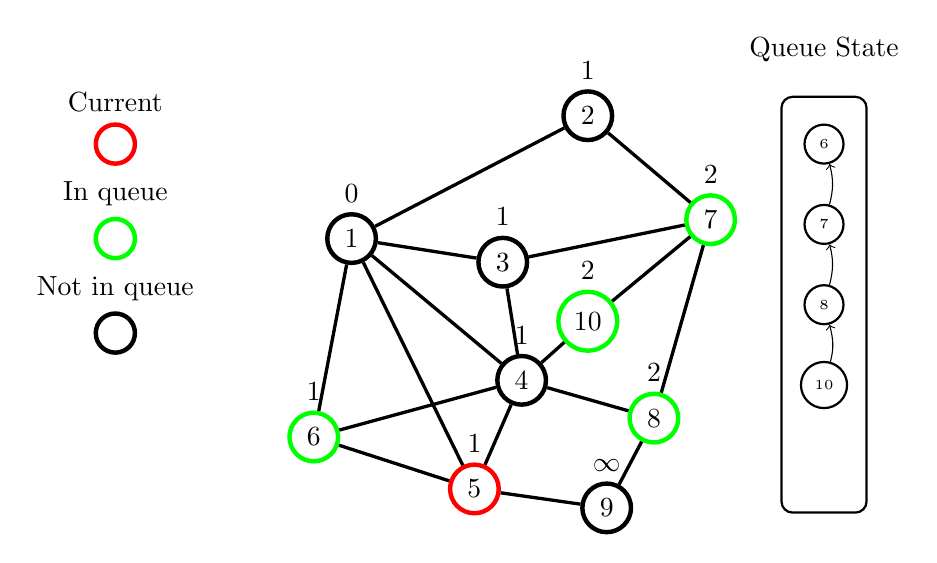
\begin{tikzpicture}[scale=1.2] 
\node[shape=circle, draw=red, 	ultra thick, scale=1.5pt, label={Current}] (U) at (-2.5, 1) {}; 
\node[shape=circle, draw=green,  ultra thick, scale=1.5pt, label={In queue}] (U) at (-2.5, 0) {}; 
\node[shape=circle, draw=black, ultra thick, scale=1.5pt, label={Not in queue}] (U) at (-2.5, -1) {}; 
\draw[thick, rounded corners,draw=black] (4.55, 1.5) rectangle ++(0.9, -1-4*0.85 );
\node[draw=white] at (5, 2) {Queue State} ; 
\node[shape=circle, draw=black, thick, minimum size=2pt] (U0) at (5, 1.0) {\tiny{6}}; 
\node[shape=circle, draw=black, thick, minimum size=2pt] (U1) at (5, 0.15000000000000002) {\tiny{7}}; 
\node[shape=circle, draw=black, thick, minimum size=2pt] (U2) at (5, -0.7) {\tiny{8}}; 
\node[shape=circle, draw=black, thick, minimum size=2pt] (U3) at (5, -1.5499999999999998) {\tiny{10}}; 
\path[->] (U1) edge [out=75, in=-75] (U0);
\path[->] (U2) edge [out=75, in=-75] (U1);
\path[->] (U3) edge [out=75, in=-75] (U2);
\node[shape=circle,draw=black, ultra thick, label={$0$}] (1) at (0,0) {1}; 
\node[shape=circle,draw=black, ultra thick, label={$1$}] (2) at (2.5,1.3) {2}; 
\node[shape=circle,draw=black, ultra thick, label={$1$}] (3) at (1.6,-0.25) {3}; 
\node[shape=circle,draw=black, ultra thick, label={$1$}] (4) at (1.8,-1.5) {4}; 
\node[shape=circle,draw=red, ultra thick, label={$1$}] (5) at (1.3,-2.65) {5}; 
\node[shape=circle,draw=green, ultra thick, label={$1$}] (6) at (-0.4,-2.1) {6}; 
\node[shape=circle,draw=green, ultra thick, label={$2$}] (7) at (3.8,0.2) {7}; 
\node[shape=circle,draw=green, ultra thick, label={$2$}] (8) at (3.2,-1.9) {8}; 
\node[shape=circle,draw=black, ultra thick, label={$\infty$}] (9) at (2.7,-2.85) {9}; 
\node[shape=circle,draw=green, ultra thick, label={$2$}] (10) at (2.5,-0.875) {10}; 
\path [-,very thick, draw=black] (1) edge  (2);
\path [-,very thick, draw=black] (1) edge  (3);
\path [-,very thick, draw=black] (1) edge  (4);
\path [-,very thick, draw=black] (1) edge  (5);
\path [-,very thick, draw=black] (1) edge  (6);
\path [-,very thick, draw=black] (2) edge  (7);
\path [-,very thick, draw=black] (3) edge  (7);
\path [-,very thick, draw=black] (3) edge  (4);
\path [-,very thick, draw=black] (4) edge  (5);
\path [-,very thick, draw=black] (4) edge  (6);
\path [-,very thick, draw=black] (4) edge  (8);
\path [-,very thick, draw=black] (4) edge  (10);
\path [-,very thick, draw=black] (5) edge  (6);
\path [-,very thick, draw=black] (5) edge  (9);
\path [-,very thick, draw=black] (7) edge  (8);
\path [-,very thick, draw=black] (7) edge  (10);
\path [-,very thick, draw=black] (8) edge  (9);
\end{tikzpicture} 
\end{figure} 
\end{frame} 
\begin{frame}{BFS : Example}
\begin{figure}
\vspace*{-1cm} 
\center
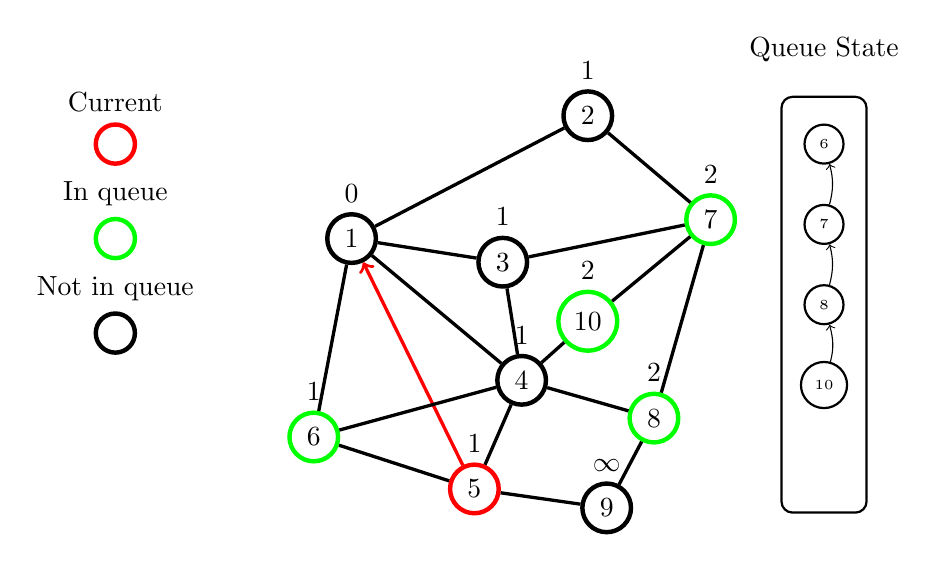
\begin{tikzpicture}[scale=1.2] 
\node[shape=circle, draw=red, 	ultra thick, scale=1.5pt, label={Current}] (U) at (-2.5, 1) {}; 
\node[shape=circle, draw=green,  ultra thick, scale=1.5pt, label={In queue}] (U) at (-2.5, 0) {}; 
\node[shape=circle, draw=black, ultra thick, scale=1.5pt, label={Not in queue}] (U) at (-2.5, -1) {}; 
\draw[thick, rounded corners,draw=black] (4.55, 1.5) rectangle ++(0.9, -1-4*0.85 );
\node[draw=white] at (5, 2) {Queue State} ; 
\node[shape=circle, draw=black, thick, minimum size=2pt] (U0) at (5, 1.0) {\tiny{6}}; 
\node[shape=circle, draw=black, thick, minimum size=2pt] (U1) at (5, 0.15000000000000002) {\tiny{7}}; 
\node[shape=circle, draw=black, thick, minimum size=2pt] (U2) at (5, -0.7) {\tiny{8}}; 
\node[shape=circle, draw=black, thick, minimum size=2pt] (U3) at (5, -1.5499999999999998) {\tiny{10}}; 
\path[->] (U1) edge [out=75, in=-75] (U0);
\path[->] (U2) edge [out=75, in=-75] (U1);
\path[->] (U3) edge [out=75, in=-75] (U2);
\node[shape=circle,draw=black, ultra thick, label={$0$}] (1) at (0,0) {1}; 
\node[shape=circle,draw=black, ultra thick, label={$1$}] (2) at (2.5,1.3) {2}; 
\node[shape=circle,draw=black, ultra thick, label={$1$}] (3) at (1.6,-0.25) {3}; 
\node[shape=circle,draw=black, ultra thick, label={$1$}] (4) at (1.8,-1.5) {4}; 
\node[shape=circle,draw=red, ultra thick, label={$1$}] (5) at (1.3,-2.65) {5}; 
\node[shape=circle,draw=green, ultra thick, label={$1$}] (6) at (-0.4,-2.1) {6}; 
\node[shape=circle,draw=green, ultra thick, label={$2$}] (7) at (3.8,0.2) {7}; 
\node[shape=circle,draw=green, ultra thick, label={$2$}] (8) at (3.2,-1.9) {8}; 
\node[shape=circle,draw=black, ultra thick, label={$\infty$}] (9) at (2.7,-2.85) {9}; 
\node[shape=circle,draw=green, ultra thick, label={$2$}] (10) at (2.5,-0.875) {10}; 
\path [-,very thick, draw=black] (1) edge  (2);
\path [-,very thick, draw=black] (1) edge  (3);
\path [-,very thick, draw=black] (1) edge  (4);
\path [->,very thick, draw=red] (5) edge  (1);
\path [-,very thick, draw=black] (1) edge  (6);
\path [-,very thick, draw=black] (2) edge  (7);
\path [-,very thick, draw=black] (3) edge  (7);
\path [-,very thick, draw=black] (3) edge  (4);
\path [-,very thick, draw=black] (4) edge  (5);
\path [-,very thick, draw=black] (4) edge  (6);
\path [-,very thick, draw=black] (4) edge  (8);
\path [-,very thick, draw=black] (4) edge  (10);
\path [-,very thick, draw=black] (5) edge  (6);
\path [-,very thick, draw=black] (5) edge  (9);
\path [-,very thick, draw=black] (7) edge  (8);
\path [-,very thick, draw=black] (7) edge  (10);
\path [-,very thick, draw=black] (8) edge  (9);
\end{tikzpicture} 
\end{figure} 
\end{frame} 
\begin{frame}{BFS : Example}
\begin{figure}
\vspace*{-1cm} 
\center
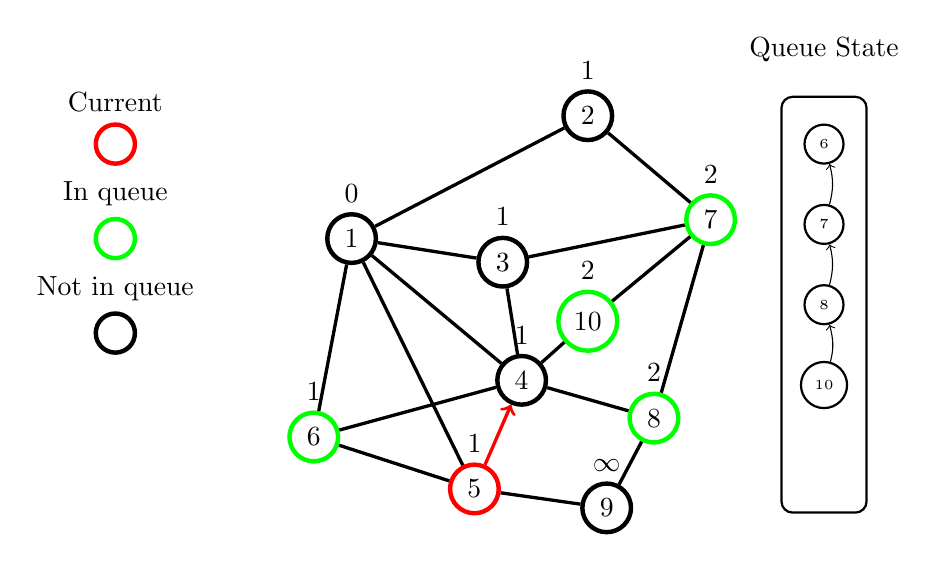
\begin{tikzpicture}[scale=1.2] 
\node[shape=circle, draw=red, 	ultra thick, scale=1.5pt, label={Current}] (U) at (-2.5, 1) {}; 
\node[shape=circle, draw=green,  ultra thick, scale=1.5pt, label={In queue}] (U) at (-2.5, 0) {}; 
\node[shape=circle, draw=black, ultra thick, scale=1.5pt, label={Not in queue}] (U) at (-2.5, -1) {}; 
\draw[thick, rounded corners,draw=black] (4.55, 1.5) rectangle ++(0.9, -1-4*0.85 );
\node[draw=white] at (5, 2) {Queue State} ; 
\node[shape=circle, draw=black, thick, minimum size=2pt] (U0) at (5, 1.0) {\tiny{6}}; 
\node[shape=circle, draw=black, thick, minimum size=2pt] (U1) at (5, 0.15000000000000002) {\tiny{7}}; 
\node[shape=circle, draw=black, thick, minimum size=2pt] (U2) at (5, -0.7) {\tiny{8}}; 
\node[shape=circle, draw=black, thick, minimum size=2pt] (U3) at (5, -1.5499999999999998) {\tiny{10}}; 
\path[->] (U1) edge [out=75, in=-75] (U0);
\path[->] (U2) edge [out=75, in=-75] (U1);
\path[->] (U3) edge [out=75, in=-75] (U2);
\node[shape=circle,draw=black, ultra thick, label={$0$}] (1) at (0,0) {1}; 
\node[shape=circle,draw=black, ultra thick, label={$1$}] (2) at (2.5,1.3) {2}; 
\node[shape=circle,draw=black, ultra thick, label={$1$}] (3) at (1.6,-0.25) {3}; 
\node[shape=circle,draw=black, ultra thick, label={$1$}] (4) at (1.8,-1.5) {4}; 
\node[shape=circle,draw=red, ultra thick, label={$1$}] (5) at (1.3,-2.65) {5}; 
\node[shape=circle,draw=green, ultra thick, label={$1$}] (6) at (-0.4,-2.1) {6}; 
\node[shape=circle,draw=green, ultra thick, label={$2$}] (7) at (3.8,0.2) {7}; 
\node[shape=circle,draw=green, ultra thick, label={$2$}] (8) at (3.2,-1.9) {8}; 
\node[shape=circle,draw=black, ultra thick, label={$\infty$}] (9) at (2.7,-2.85) {9}; 
\node[shape=circle,draw=green, ultra thick, label={$2$}] (10) at (2.5,-0.875) {10}; 
\path [-,very thick, draw=black] (1) edge  (2);
\path [-,very thick, draw=black] (1) edge  (3);
\path [-,very thick, draw=black] (1) edge  (4);
\path [-,very thick, draw=black] (1) edge  (5);
\path [-,very thick, draw=black] (1) edge  (6);
\path [-,very thick, draw=black] (2) edge  (7);
\path [-,very thick, draw=black] (3) edge  (7);
\path [-,very thick, draw=black] (3) edge  (4);
\path [->,very thick, draw=red] (5) edge  (4);
\path [-,very thick, draw=black] (4) edge  (6);
\path [-,very thick, draw=black] (4) edge  (8);
\path [-,very thick, draw=black] (4) edge  (10);
\path [-,very thick, draw=black] (5) edge  (6);
\path [-,very thick, draw=black] (5) edge  (9);
\path [-,very thick, draw=black] (7) edge  (8);
\path [-,very thick, draw=black] (7) edge  (10);
\path [-,very thick, draw=black] (8) edge  (9);
\end{tikzpicture} 
\end{figure} 
\end{frame} 
\begin{frame}{BFS : Example}
\begin{figure}
\vspace*{-1cm} 
\center
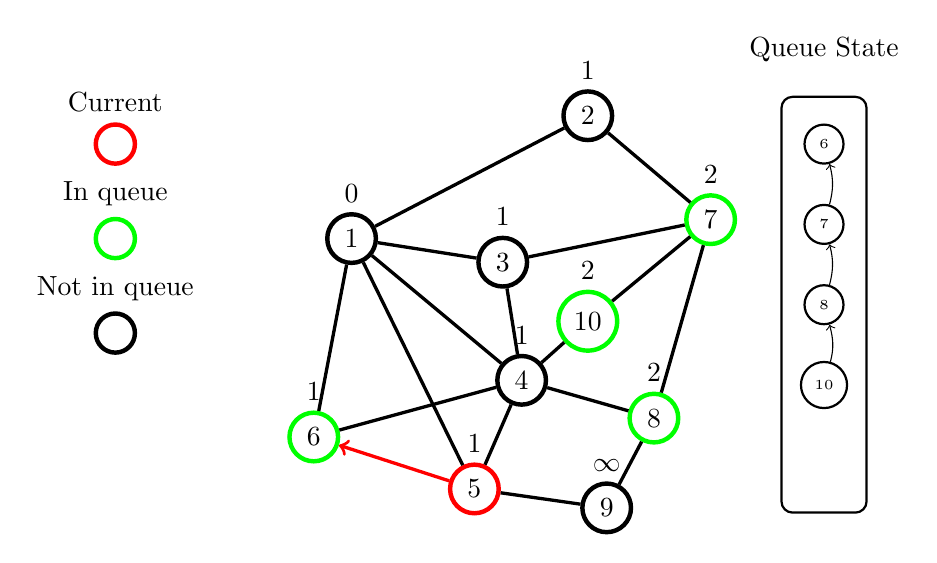
\begin{tikzpicture}[scale=1.2] 
\node[shape=circle, draw=red, 	ultra thick, scale=1.5pt, label={Current}] (U) at (-2.5, 1) {}; 
\node[shape=circle, draw=green,  ultra thick, scale=1.5pt, label={In queue}] (U) at (-2.5, 0) {}; 
\node[shape=circle, draw=black, ultra thick, scale=1.5pt, label={Not in queue}] (U) at (-2.5, -1) {}; 
\draw[thick, rounded corners,draw=black] (4.55, 1.5) rectangle ++(0.9, -1-4*0.85 );
\node[draw=white] at (5, 2) {Queue State} ; 
\node[shape=circle, draw=black, thick, minimum size=2pt] (U0) at (5, 1.0) {\tiny{6}}; 
\node[shape=circle, draw=black, thick, minimum size=2pt] (U1) at (5, 0.15000000000000002) {\tiny{7}}; 
\node[shape=circle, draw=black, thick, minimum size=2pt] (U2) at (5, -0.7) {\tiny{8}}; 
\node[shape=circle, draw=black, thick, minimum size=2pt] (U3) at (5, -1.5499999999999998) {\tiny{10}}; 
\path[->] (U1) edge [out=75, in=-75] (U0);
\path[->] (U2) edge [out=75, in=-75] (U1);
\path[->] (U3) edge [out=75, in=-75] (U2);
\node[shape=circle,draw=black, ultra thick, label={$0$}] (1) at (0,0) {1}; 
\node[shape=circle,draw=black, ultra thick, label={$1$}] (2) at (2.5,1.3) {2}; 
\node[shape=circle,draw=black, ultra thick, label={$1$}] (3) at (1.6,-0.25) {3}; 
\node[shape=circle,draw=black, ultra thick, label={$1$}] (4) at (1.8,-1.5) {4}; 
\node[shape=circle,draw=red, ultra thick, label={$1$}] (5) at (1.3,-2.65) {5}; 
\node[shape=circle,draw=green, ultra thick, label={$1$}] (6) at (-0.4,-2.1) {6}; 
\node[shape=circle,draw=green, ultra thick, label={$2$}] (7) at (3.8,0.2) {7}; 
\node[shape=circle,draw=green, ultra thick, label={$2$}] (8) at (3.2,-1.9) {8}; 
\node[shape=circle,draw=black, ultra thick, label={$\infty$}] (9) at (2.7,-2.85) {9}; 
\node[shape=circle,draw=green, ultra thick, label={$2$}] (10) at (2.5,-0.875) {10}; 
\path [-,very thick, draw=black] (1) edge  (2);
\path [-,very thick, draw=black] (1) edge  (3);
\path [-,very thick, draw=black] (1) edge  (4);
\path [-,very thick, draw=black] (1) edge  (5);
\path [-,very thick, draw=black] (1) edge  (6);
\path [-,very thick, draw=black] (2) edge  (7);
\path [-,very thick, draw=black] (3) edge  (7);
\path [-,very thick, draw=black] (3) edge  (4);
\path [-,very thick, draw=black] (4) edge  (5);
\path [-,very thick, draw=black] (4) edge  (6);
\path [-,very thick, draw=black] (4) edge  (8);
\path [-,very thick, draw=black] (4) edge  (10);
\path [->,very thick, draw=red] (5) edge  (6);
\path [-,very thick, draw=black] (5) edge  (9);
\path [-,very thick, draw=black] (7) edge  (8);
\path [-,very thick, draw=black] (7) edge  (10);
\path [-,very thick, draw=black] (8) edge  (9);
\end{tikzpicture} 
\end{figure} 
\end{frame} 
\begin{frame}{BFS : Example}
\begin{figure}
\vspace*{-1cm} 
\center
\begin{tikzpicture}[scale=1.2] 
\node[shape=circle, draw=red, 	ultra thick, scale=1.5pt, label={Current}] (U) at (-2.5, 1) {}; 
\node[shape=circle, draw=green,  ultra thick, scale=1.5pt, label={In queue}] (U) at (-2.5, 0) {}; 
\node[shape=circle, draw=black, ultra thick, scale=1.5pt, label={Not in queue}] (U) at (-2.5, -1) {}; 
\draw[thick, rounded corners,draw=black] (4.55, 1.5) rectangle ++(0.9, -1-4*0.85 );
\node[draw=white] at (5, 2) {Queue State} ; 
\node[shape=circle, draw=black, thick, minimum size=2pt] (U0) at (5, 1.0) {\tiny{6}}; 
\node[shape=circle, draw=black, thick, minimum size=2pt] (U1) at (5, 0.15000000000000002) {\tiny{7}}; 
\node[shape=circle, draw=black, thick, minimum size=2pt] (U2) at (5, -0.7) {\tiny{8}}; 
\node[shape=circle, draw=black, thick, minimum size=2pt] (U3) at (5, -1.5499999999999998) {\tiny{10}}; 
\node[shape=circle, draw=black, thick, minimum size=2pt] (U4) at (5, -2.4) {\tiny{9}}; 
\path[->] (U1) edge [out=75, in=-75] (U0);
\path[->] (U2) edge [out=75, in=-75] (U1);
\path[->] (U3) edge [out=75, in=-75] (U2);
\path[->] (U4) edge [out=75, in=-75] (U3);
\path[->, thick, draw=black] (9) edge [dashed, bend right=30] (U4); 
\node[shape=circle,draw=black, ultra thick, label={$0$}] (1) at (0,0) {1}; 
\node[shape=circle,draw=black, ultra thick, label={$1$}] (2) at (2.5,1.3) {2}; 
\node[shape=circle,draw=black, ultra thick, label={$1$}] (3) at (1.6,-0.25) {3}; 
\node[shape=circle,draw=black, ultra thick, label={$1$}] (4) at (1.8,-1.5) {4}; 
\node[shape=circle,draw=red, ultra thick, label={$1$}] (5) at (1.3,-2.65) {5}; 
\node[shape=circle,draw=green, ultra thick, label={$1$}] (6) at (-0.4,-2.1) {6}; 
\node[shape=circle,draw=green, ultra thick, label={$2$}] (7) at (3.8,0.2) {7}; 
\node[shape=circle,draw=green, ultra thick, label={$2$}] (8) at (3.2,-1.9) {8}; 
\node[shape=circle,draw=green, ultra thick, label={$2$}] (9) at (2.7,-2.85) {9}; 
\node[shape=circle,draw=green, ultra thick, label={$2$}] (10) at (2.5,-0.875) {10}; 
\path [-,very thick, draw=black] (1) edge  (2);
\path [-,very thick, draw=black] (1) edge  (3);
\path [-,very thick, draw=black] (1) edge  (4);
\path [-,very thick, draw=black] (1) edge  (5);
\path [-,very thick, draw=black] (1) edge  (6);
\path [-,very thick, draw=black] (2) edge  (7);
\path [-,very thick, draw=black] (3) edge  (7);
\path [-,very thick, draw=black] (3) edge  (4);
\path [-,very thick, draw=black] (4) edge  (5);
\path [-,very thick, draw=black] (4) edge  (6);
\path [-,very thick, draw=black] (4) edge  (8);
\path [-,very thick, draw=black] (4) edge  (10);
\path [-,very thick, draw=black] (5) edge  (6);
\path [->,very thick, draw=red] (5) edge  (9);
\path [-,very thick, draw=black] (7) edge  (8);
\path [-,very thick, draw=black] (7) edge  (10);
\path [-,very thick, draw=black] (8) edge  (9);
\end{tikzpicture} 
\end{figure} 
\end{frame} 
\begin{frame}{BFS : Example}
\begin{figure}
\vspace*{-1cm} 
\center
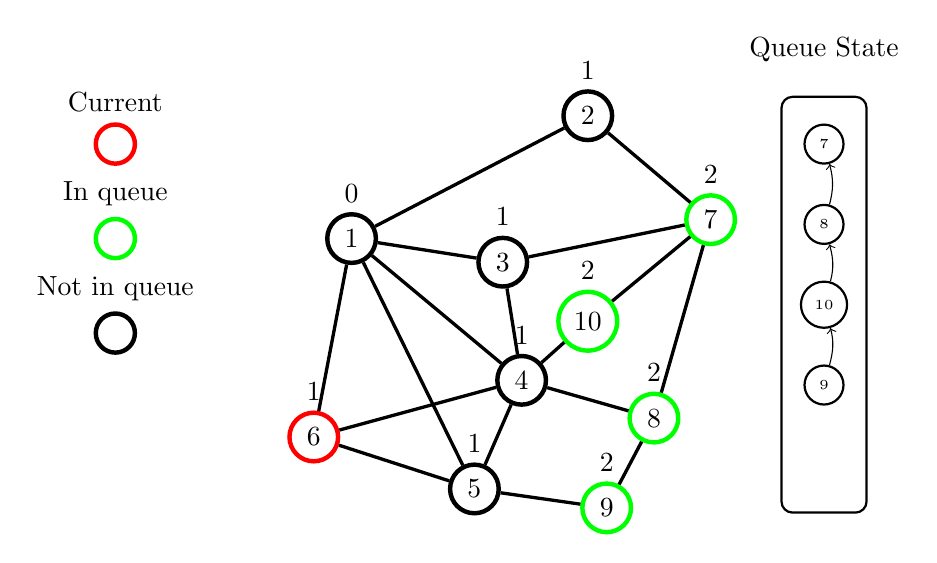
\begin{tikzpicture}[scale=1.2] 
\node[shape=circle, draw=red, 	ultra thick, scale=1.5pt, label={Current}] (U) at (-2.5, 1) {}; 
\node[shape=circle, draw=green,  ultra thick, scale=1.5pt, label={In queue}] (U) at (-2.5, 0) {}; 
\node[shape=circle, draw=black, ultra thick, scale=1.5pt, label={Not in queue}] (U) at (-2.5, -1) {}; 
\draw[thick, rounded corners,draw=black] (4.55, 1.5) rectangle ++(0.9, -1-4*0.85 );
\node[draw=white] at (5, 2) {Queue State} ; 
\node[shape=circle, draw=black, thick, minimum size=2pt] (U0) at (5, 1.0) {\tiny{7}}; 
\node[shape=circle, draw=black, thick, minimum size=2pt] (U1) at (5, 0.15000000000000002) {\tiny{8}}; 
\node[shape=circle, draw=black, thick, minimum size=2pt] (U2) at (5, -0.7) {\tiny{10}}; 
\node[shape=circle, draw=black, thick, minimum size=2pt] (U3) at (5, -1.5499999999999998) {\tiny{9}}; 
\path[->] (U1) edge [out=75, in=-75] (U0);
\path[->] (U2) edge [out=75, in=-75] (U1);
\path[->] (U3) edge [out=75, in=-75] (U2);
\node[shape=circle,draw=black, ultra thick, label={$0$}] (1) at (0,0) {1}; 
\node[shape=circle,draw=black, ultra thick, label={$1$}] (2) at (2.5,1.3) {2}; 
\node[shape=circle,draw=black, ultra thick, label={$1$}] (3) at (1.6,-0.25) {3}; 
\node[shape=circle,draw=black, ultra thick, label={$1$}] (4) at (1.8,-1.5) {4}; 
\node[shape=circle,draw=black, ultra thick, label={$1$}] (5) at (1.3,-2.65) {5}; 
\node[shape=circle,draw=red, ultra thick, label={$1$}] (6) at (-0.4,-2.1) {6}; 
\node[shape=circle,draw=green, ultra thick, label={$2$}] (7) at (3.8,0.2) {7}; 
\node[shape=circle,draw=green, ultra thick, label={$2$}] (8) at (3.2,-1.9) {8}; 
\node[shape=circle,draw=green, ultra thick, label={$2$}] (9) at (2.7,-2.85) {9}; 
\node[shape=circle,draw=green, ultra thick, label={$2$}] (10) at (2.5,-0.875) {10}; 
\path [-,very thick, draw=black] (1) edge  (2);
\path [-,very thick, draw=black] (1) edge  (3);
\path [-,very thick, draw=black] (1) edge  (4);
\path [-,very thick, draw=black] (1) edge  (5);
\path [-,very thick, draw=black] (1) edge  (6);
\path [-,very thick, draw=black] (2) edge  (7);
\path [-,very thick, draw=black] (3) edge  (7);
\path [-,very thick, draw=black] (3) edge  (4);
\path [-,very thick, draw=black] (4) edge  (5);
\path [-,very thick, draw=black] (4) edge  (6);
\path [-,very thick, draw=black] (4) edge  (8);
\path [-,very thick, draw=black] (4) edge  (10);
\path [-,very thick, draw=black] (5) edge  (6);
\path [-,very thick, draw=black] (5) edge  (9);
\path [-,very thick, draw=black] (7) edge  (8);
\path [-,very thick, draw=black] (7) edge  (10);
\path [-,very thick, draw=black] (8) edge  (9);
\end{tikzpicture} 
\end{figure} 
\end{frame} 
\begin{frame}{BFS : Example}
\begin{figure}
\vspace*{-1cm} 
\center
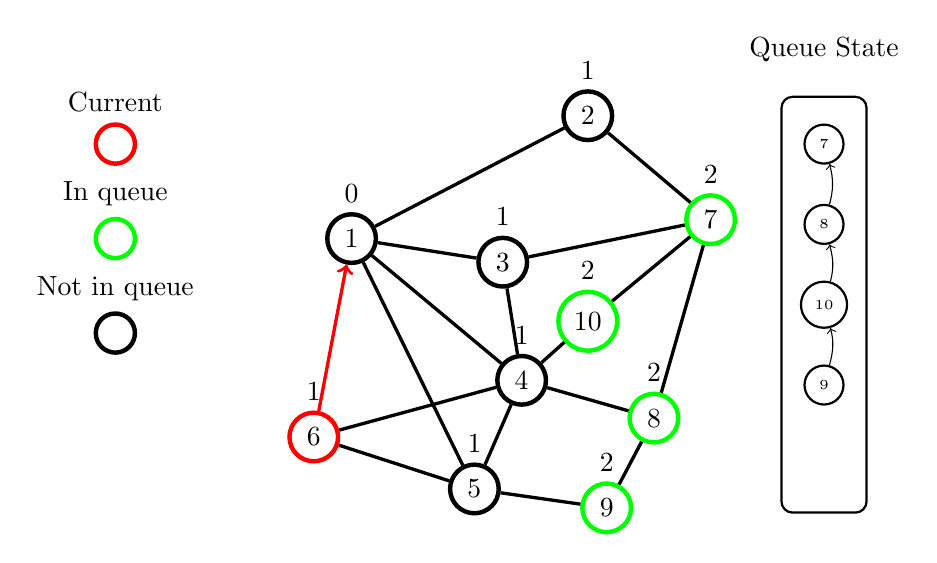
\begin{tikzpicture}[scale=1.2] 
\node[shape=circle, draw=red, 	ultra thick, scale=1.5pt, label={Current}] (U) at (-2.5, 1) {}; 
\node[shape=circle, draw=green,  ultra thick, scale=1.5pt, label={In queue}] (U) at (-2.5, 0) {}; 
\node[shape=circle, draw=black, ultra thick, scale=1.5pt, label={Not in queue}] (U) at (-2.5, -1) {}; 
\draw[thick, rounded corners,draw=black] (4.55, 1.5) rectangle ++(0.9, -1-4*0.85 );
\node[draw=white] at (5, 2) {Queue State} ; 
\node[shape=circle, draw=black, thick, minimum size=2pt] (U0) at (5, 1.0) {\tiny{7}}; 
\node[shape=circle, draw=black, thick, minimum size=2pt] (U1) at (5, 0.15000000000000002) {\tiny{8}}; 
\node[shape=circle, draw=black, thick, minimum size=2pt] (U2) at (5, -0.7) {\tiny{10}}; 
\node[shape=circle, draw=black, thick, minimum size=2pt] (U3) at (5, -1.5499999999999998) {\tiny{9}}; 
\path[->] (U1) edge [out=75, in=-75] (U0);
\path[->] (U2) edge [out=75, in=-75] (U1);
\path[->] (U3) edge [out=75, in=-75] (U2);
\node[shape=circle,draw=black, ultra thick, label={$0$}] (1) at (0,0) {1}; 
\node[shape=circle,draw=black, ultra thick, label={$1$}] (2) at (2.5,1.3) {2}; 
\node[shape=circle,draw=black, ultra thick, label={$1$}] (3) at (1.6,-0.25) {3}; 
\node[shape=circle,draw=black, ultra thick, label={$1$}] (4) at (1.8,-1.5) {4}; 
\node[shape=circle,draw=black, ultra thick, label={$1$}] (5) at (1.3,-2.65) {5}; 
\node[shape=circle,draw=red, ultra thick, label={$1$}] (6) at (-0.4,-2.1) {6}; 
\node[shape=circle,draw=green, ultra thick, label={$2$}] (7) at (3.8,0.2) {7}; 
\node[shape=circle,draw=green, ultra thick, label={$2$}] (8) at (3.2,-1.9) {8}; 
\node[shape=circle,draw=green, ultra thick, label={$2$}] (9) at (2.7,-2.85) {9}; 
\node[shape=circle,draw=green, ultra thick, label={$2$}] (10) at (2.5,-0.875) {10}; 
\path [-,very thick, draw=black] (1) edge  (2);
\path [-,very thick, draw=black] (1) edge  (3);
\path [-,very thick, draw=black] (1) edge  (4);
\path [-,very thick, draw=black] (1) edge  (5);
\path [->,very thick, draw=red] (6) edge  (1);
\path [-,very thick, draw=black] (2) edge  (7);
\path [-,very thick, draw=black] (3) edge  (7);
\path [-,very thick, draw=black] (3) edge  (4);
\path [-,very thick, draw=black] (4) edge  (5);
\path [-,very thick, draw=black] (4) edge  (6);
\path [-,very thick, draw=black] (4) edge  (8);
\path [-,very thick, draw=black] (4) edge  (10);
\path [-,very thick, draw=black] (5) edge  (6);
\path [-,very thick, draw=black] (5) edge  (9);
\path [-,very thick, draw=black] (7) edge  (8);
\path [-,very thick, draw=black] (7) edge  (10);
\path [-,very thick, draw=black] (8) edge  (9);
\end{tikzpicture} 
\end{figure} 
\end{frame} 
\begin{frame}{BFS : Example}
\begin{figure}
\vspace*{-1cm} 
\center
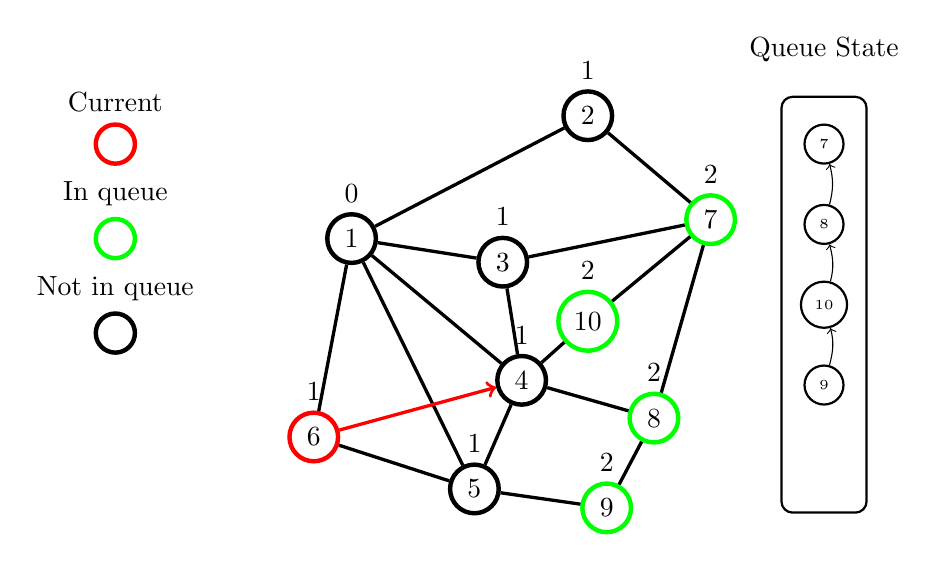
\begin{tikzpicture}[scale=1.2] 
\node[shape=circle, draw=red, 	ultra thick, scale=1.5pt, label={Current}] (U) at (-2.5, 1) {}; 
\node[shape=circle, draw=green,  ultra thick, scale=1.5pt, label={In queue}] (U) at (-2.5, 0) {}; 
\node[shape=circle, draw=black, ultra thick, scale=1.5pt, label={Not in queue}] (U) at (-2.5, -1) {}; 
\draw[thick, rounded corners,draw=black] (4.55, 1.5) rectangle ++(0.9, -1-4*0.85 );
\node[draw=white] at (5, 2) {Queue State} ; 
\node[shape=circle, draw=black, thick, minimum size=2pt] (U0) at (5, 1.0) {\tiny{7}}; 
\node[shape=circle, draw=black, thick, minimum size=2pt] (U1) at (5, 0.15000000000000002) {\tiny{8}}; 
\node[shape=circle, draw=black, thick, minimum size=2pt] (U2) at (5, -0.7) {\tiny{10}}; 
\node[shape=circle, draw=black, thick, minimum size=2pt] (U3) at (5, -1.5499999999999998) {\tiny{9}}; 
\path[->] (U1) edge [out=75, in=-75] (U0);
\path[->] (U2) edge [out=75, in=-75] (U1);
\path[->] (U3) edge [out=75, in=-75] (U2);
\node[shape=circle,draw=black, ultra thick, label={$0$}] (1) at (0,0) {1}; 
\node[shape=circle,draw=black, ultra thick, label={$1$}] (2) at (2.5,1.3) {2}; 
\node[shape=circle,draw=black, ultra thick, label={$1$}] (3) at (1.6,-0.25) {3}; 
\node[shape=circle,draw=black, ultra thick, label={$1$}] (4) at (1.8,-1.5) {4}; 
\node[shape=circle,draw=black, ultra thick, label={$1$}] (5) at (1.3,-2.65) {5}; 
\node[shape=circle,draw=red, ultra thick, label={$1$}] (6) at (-0.4,-2.1) {6}; 
\node[shape=circle,draw=green, ultra thick, label={$2$}] (7) at (3.8,0.2) {7}; 
\node[shape=circle,draw=green, ultra thick, label={$2$}] (8) at (3.2,-1.9) {8}; 
\node[shape=circle,draw=green, ultra thick, label={$2$}] (9) at (2.7,-2.85) {9}; 
\node[shape=circle,draw=green, ultra thick, label={$2$}] (10) at (2.5,-0.875) {10}; 
\path [-,very thick, draw=black] (1) edge  (2);
\path [-,very thick, draw=black] (1) edge  (3);
\path [-,very thick, draw=black] (1) edge  (4);
\path [-,very thick, draw=black] (1) edge  (5);
\path [-,very thick, draw=black] (1) edge  (6);
\path [-,very thick, draw=black] (2) edge  (7);
\path [-,very thick, draw=black] (3) edge  (7);
\path [-,very thick, draw=black] (3) edge  (4);
\path [-,very thick, draw=black] (4) edge  (5);
\path [->,very thick, draw=red] (6) edge  (4);
\path [-,very thick, draw=black] (4) edge  (8);
\path [-,very thick, draw=black] (4) edge  (10);
\path [-,very thick, draw=black] (5) edge  (6);
\path [-,very thick, draw=black] (5) edge  (9);
\path [-,very thick, draw=black] (7) edge  (8);
\path [-,very thick, draw=black] (7) edge  (10);
\path [-,very thick, draw=black] (8) edge  (9);
\end{tikzpicture} 
\end{figure} 
\end{frame} 
\begin{frame}{BFS : Example}
\begin{figure}
\vspace*{-1cm} 
\center
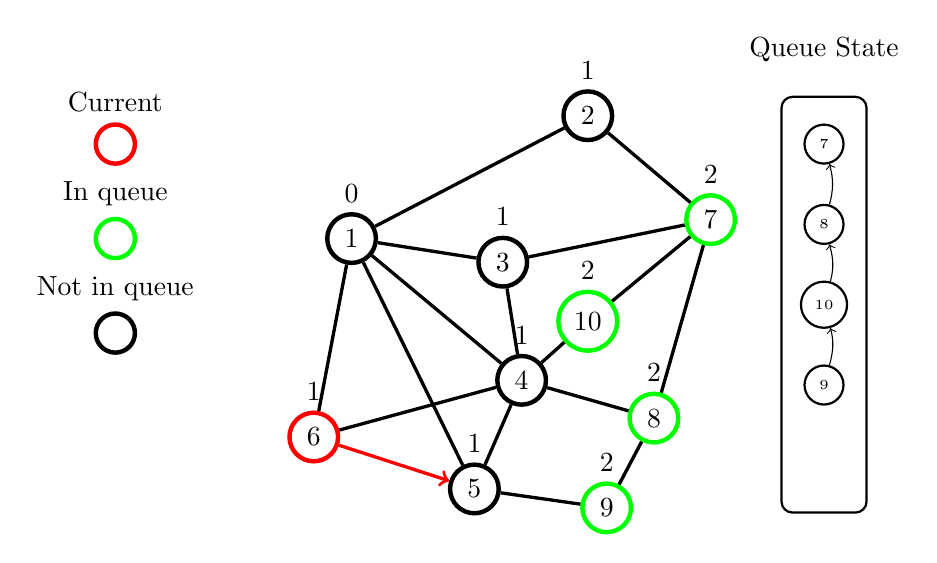
\begin{tikzpicture}[scale=1.2] 
\node[shape=circle, draw=red, 	ultra thick, scale=1.5pt, label={Current}] (U) at (-2.5, 1) {}; 
\node[shape=circle, draw=green,  ultra thick, scale=1.5pt, label={In queue}] (U) at (-2.5, 0) {}; 
\node[shape=circle, draw=black, ultra thick, scale=1.5pt, label={Not in queue}] (U) at (-2.5, -1) {}; 
\draw[thick, rounded corners,draw=black] (4.55, 1.5) rectangle ++(0.9, -1-4*0.85 );
\node[draw=white] at (5, 2) {Queue State} ; 
\node[shape=circle, draw=black, thick, minimum size=2pt] (U0) at (5, 1.0) {\tiny{7}}; 
\node[shape=circle, draw=black, thick, minimum size=2pt] (U1) at (5, 0.15000000000000002) {\tiny{8}}; 
\node[shape=circle, draw=black, thick, minimum size=2pt] (U2) at (5, -0.7) {\tiny{10}}; 
\node[shape=circle, draw=black, thick, minimum size=2pt] (U3) at (5, -1.5499999999999998) {\tiny{9}}; 
\path[->] (U1) edge [out=75, in=-75] (U0);
\path[->] (U2) edge [out=75, in=-75] (U1);
\path[->] (U3) edge [out=75, in=-75] (U2);
\node[shape=circle,draw=black, ultra thick, label={$0$}] (1) at (0,0) {1}; 
\node[shape=circle,draw=black, ultra thick, label={$1$}] (2) at (2.5,1.3) {2}; 
\node[shape=circle,draw=black, ultra thick, label={$1$}] (3) at (1.6,-0.25) {3}; 
\node[shape=circle,draw=black, ultra thick, label={$1$}] (4) at (1.8,-1.5) {4}; 
\node[shape=circle,draw=black, ultra thick, label={$1$}] (5) at (1.3,-2.65) {5}; 
\node[shape=circle,draw=red, ultra thick, label={$1$}] (6) at (-0.4,-2.1) {6}; 
\node[shape=circle,draw=green, ultra thick, label={$2$}] (7) at (3.8,0.2) {7}; 
\node[shape=circle,draw=green, ultra thick, label={$2$}] (8) at (3.2,-1.9) {8}; 
\node[shape=circle,draw=green, ultra thick, label={$2$}] (9) at (2.7,-2.85) {9}; 
\node[shape=circle,draw=green, ultra thick, label={$2$}] (10) at (2.5,-0.875) {10}; 
\path [-,very thick, draw=black] (1) edge  (2);
\path [-,very thick, draw=black] (1) edge  (3);
\path [-,very thick, draw=black] (1) edge  (4);
\path [-,very thick, draw=black] (1) edge  (5);
\path [-,very thick, draw=black] (1) edge  (6);
\path [-,very thick, draw=black] (2) edge  (7);
\path [-,very thick, draw=black] (3) edge  (7);
\path [-,very thick, draw=black] (3) edge  (4);
\path [-,very thick, draw=black] (4) edge  (5);
\path [-,very thick, draw=black] (4) edge  (6);
\path [-,very thick, draw=black] (4) edge  (8);
\path [-,very thick, draw=black] (4) edge  (10);
\path [->,very thick, draw=red] (6) edge  (5);
\path [-,very thick, draw=black] (5) edge  (9);
\path [-,very thick, draw=black] (7) edge  (8);
\path [-,very thick, draw=black] (7) edge  (10);
\path [-,very thick, draw=black] (8) edge  (9);
\end{tikzpicture} 
\end{figure} 
\end{frame} 
\begin{frame}{BFS : Example}
\begin{figure}
\vspace*{-1cm} 
\center
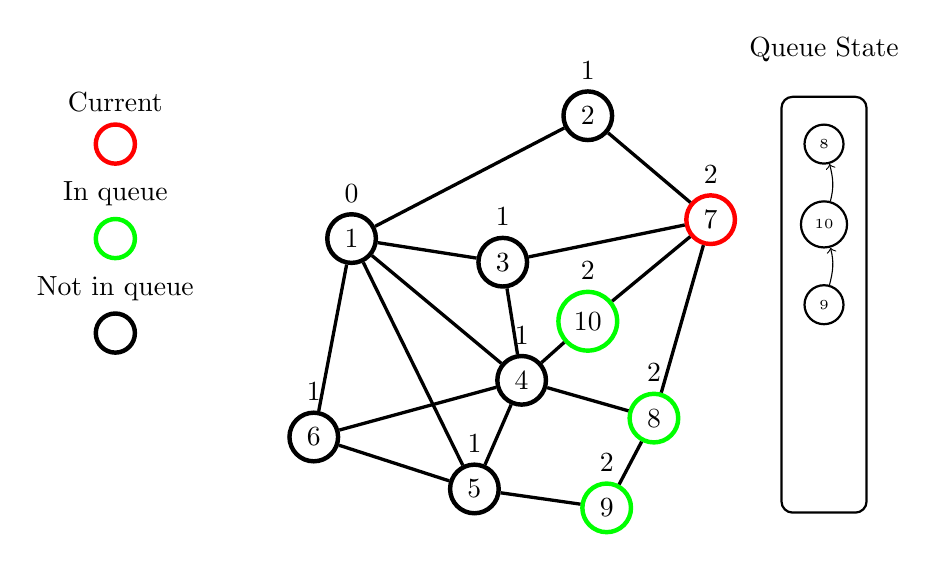
\begin{tikzpicture}[scale=1.2] 
\node[shape=circle, draw=red, 	ultra thick, scale=1.5pt, label={Current}] (U) at (-2.5, 1) {}; 
\node[shape=circle, draw=green,  ultra thick, scale=1.5pt, label={In queue}] (U) at (-2.5, 0) {}; 
\node[shape=circle, draw=black, ultra thick, scale=1.5pt, label={Not in queue}] (U) at (-2.5, -1) {}; 
\draw[thick, rounded corners,draw=black] (4.55, 1.5) rectangle ++(0.9, -1-4*0.85 );
\node[draw=white] at (5, 2) {Queue State} ; 
\node[shape=circle, draw=black, thick, minimum size=2pt] (U0) at (5, 1.0) {\tiny{8}}; 
\node[shape=circle, draw=black, thick, minimum size=2pt] (U1) at (5, 0.15000000000000002) {\tiny{10}}; 
\node[shape=circle, draw=black, thick, minimum size=2pt] (U2) at (5, -0.7) {\tiny{9}}; 
\path[->] (U1) edge [out=75, in=-75] (U0);
\path[->] (U2) edge [out=75, in=-75] (U1);
\node[shape=circle,draw=black, ultra thick, label={$0$}] (1) at (0,0) {1}; 
\node[shape=circle,draw=black, ultra thick, label={$1$}] (2) at (2.5,1.3) {2}; 
\node[shape=circle,draw=black, ultra thick, label={$1$}] (3) at (1.6,-0.25) {3}; 
\node[shape=circle,draw=black, ultra thick, label={$1$}] (4) at (1.8,-1.5) {4}; 
\node[shape=circle,draw=black, ultra thick, label={$1$}] (5) at (1.3,-2.65) {5}; 
\node[shape=circle,draw=black, ultra thick, label={$1$}] (6) at (-0.4,-2.1) {6}; 
\node[shape=circle,draw=red, ultra thick, label={$2$}] (7) at (3.8,0.2) {7}; 
\node[shape=circle,draw=green, ultra thick, label={$2$}] (8) at (3.2,-1.9) {8}; 
\node[shape=circle,draw=green, ultra thick, label={$2$}] (9) at (2.7,-2.85) {9}; 
\node[shape=circle,draw=green, ultra thick, label={$2$}] (10) at (2.5,-0.875) {10}; 
\path [-,very thick, draw=black] (1) edge  (2);
\path [-,very thick, draw=black] (1) edge  (3);
\path [-,very thick, draw=black] (1) edge  (4);
\path [-,very thick, draw=black] (1) edge  (5);
\path [-,very thick, draw=black] (1) edge  (6);
\path [-,very thick, draw=black] (2) edge  (7);
\path [-,very thick, draw=black] (3) edge  (7);
\path [-,very thick, draw=black] (3) edge  (4);
\path [-,very thick, draw=black] (4) edge  (5);
\path [-,very thick, draw=black] (4) edge  (6);
\path [-,very thick, draw=black] (4) edge  (8);
\path [-,very thick, draw=black] (4) edge  (10);
\path [-,very thick, draw=black] (5) edge  (6);
\path [-,very thick, draw=black] (5) edge  (9);
\path [-,very thick, draw=black] (7) edge  (8);
\path [-,very thick, draw=black] (7) edge  (10);
\path [-,very thick, draw=black] (8) edge  (9);
\end{tikzpicture} 
\end{figure} 
\end{frame} 
\begin{frame}{BFS : Example}
\begin{figure}
\vspace*{-1cm} 
\center
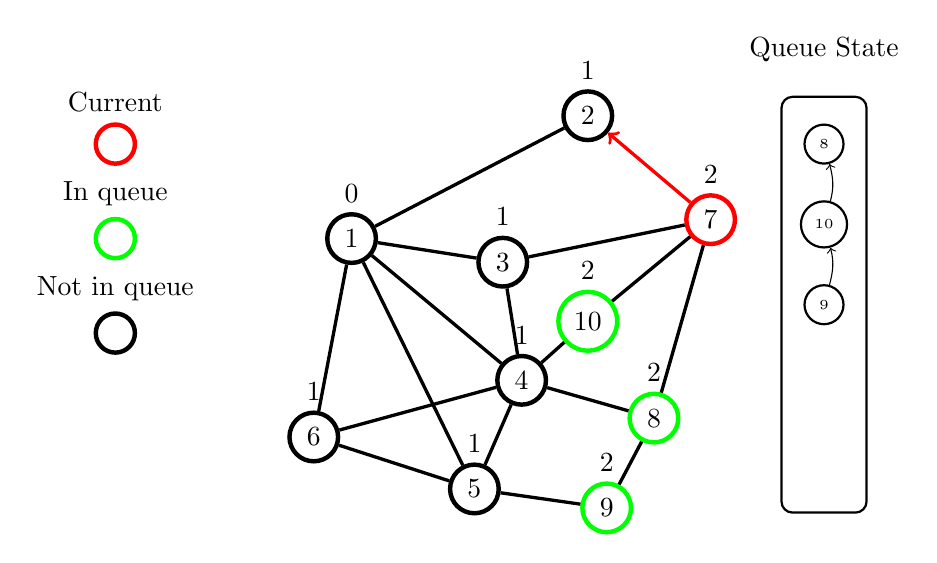
\begin{tikzpicture}[scale=1.2] 
\node[shape=circle, draw=red, 	ultra thick, scale=1.5pt, label={Current}] (U) at (-2.5, 1) {}; 
\node[shape=circle, draw=green,  ultra thick, scale=1.5pt, label={In queue}] (U) at (-2.5, 0) {}; 
\node[shape=circle, draw=black, ultra thick, scale=1.5pt, label={Not in queue}] (U) at (-2.5, -1) {}; 
\draw[thick, rounded corners,draw=black] (4.55, 1.5) rectangle ++(0.9, -1-4*0.85 );
\node[draw=white] at (5, 2) {Queue State} ; 
\node[shape=circle, draw=black, thick, minimum size=2pt] (U0) at (5, 1.0) {\tiny{8}}; 
\node[shape=circle, draw=black, thick, minimum size=2pt] (U1) at (5, 0.15000000000000002) {\tiny{10}}; 
\node[shape=circle, draw=black, thick, minimum size=2pt] (U2) at (5, -0.7) {\tiny{9}}; 
\path[->] (U1) edge [out=75, in=-75] (U0);
\path[->] (U2) edge [out=75, in=-75] (U1);
\node[shape=circle,draw=black, ultra thick, label={$0$}] (1) at (0,0) {1}; 
\node[shape=circle,draw=black, ultra thick, label={$1$}] (2) at (2.5,1.3) {2}; 
\node[shape=circle,draw=black, ultra thick, label={$1$}] (3) at (1.6,-0.25) {3}; 
\node[shape=circle,draw=black, ultra thick, label={$1$}] (4) at (1.8,-1.5) {4}; 
\node[shape=circle,draw=black, ultra thick, label={$1$}] (5) at (1.3,-2.65) {5}; 
\node[shape=circle,draw=black, ultra thick, label={$1$}] (6) at (-0.4,-2.1) {6}; 
\node[shape=circle,draw=red, ultra thick, label={$2$}] (7) at (3.8,0.2) {7}; 
\node[shape=circle,draw=green, ultra thick, label={$2$}] (8) at (3.2,-1.9) {8}; 
\node[shape=circle,draw=green, ultra thick, label={$2$}] (9) at (2.7,-2.85) {9}; 
\node[shape=circle,draw=green, ultra thick, label={$2$}] (10) at (2.5,-0.875) {10}; 
\path [-,very thick, draw=black] (1) edge  (2);
\path [-,very thick, draw=black] (1) edge  (3);
\path [-,very thick, draw=black] (1) edge  (4);
\path [-,very thick, draw=black] (1) edge  (5);
\path [-,very thick, draw=black] (1) edge  (6);
\path [->,very thick, draw=red] (7) edge  (2);
\path [-,very thick, draw=black] (3) edge  (7);
\path [-,very thick, draw=black] (3) edge  (4);
\path [-,very thick, draw=black] (4) edge  (5);
\path [-,very thick, draw=black] (4) edge  (6);
\path [-,very thick, draw=black] (4) edge  (8);
\path [-,very thick, draw=black] (4) edge  (10);
\path [-,very thick, draw=black] (5) edge  (6);
\path [-,very thick, draw=black] (5) edge  (9);
\path [-,very thick, draw=black] (7) edge  (8);
\path [-,very thick, draw=black] (7) edge  (10);
\path [-,very thick, draw=black] (8) edge  (9);
\end{tikzpicture} 
\end{figure} 
\end{frame} 
\begin{frame}{BFS : Example}
\begin{figure}
\vspace*{-1cm} 
\center
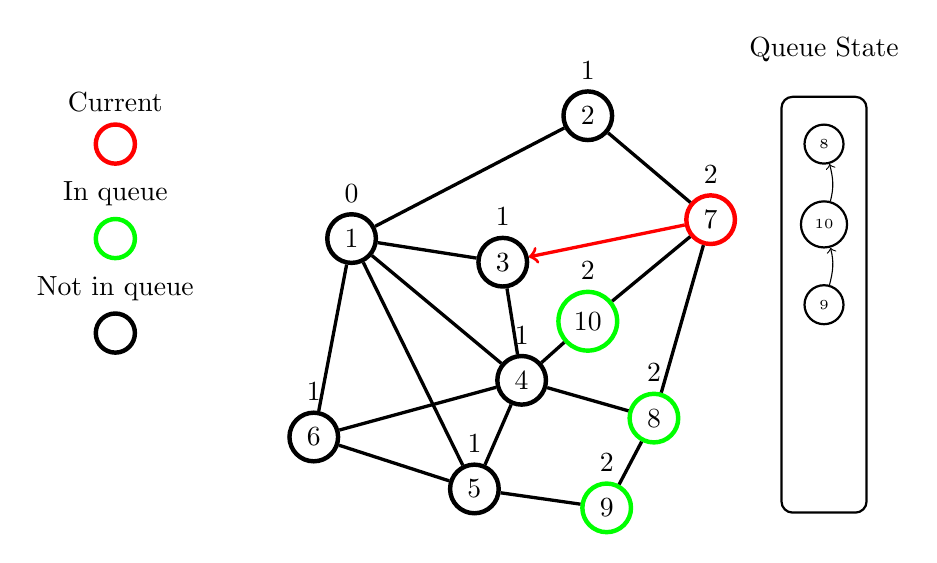
\begin{tikzpicture}[scale=1.2] 
\node[shape=circle, draw=red, 	ultra thick, scale=1.5pt, label={Current}] (U) at (-2.5, 1) {}; 
\node[shape=circle, draw=green,  ultra thick, scale=1.5pt, label={In queue}] (U) at (-2.5, 0) {}; 
\node[shape=circle, draw=black, ultra thick, scale=1.5pt, label={Not in queue}] (U) at (-2.5, -1) {}; 
\draw[thick, rounded corners,draw=black] (4.55, 1.5) rectangle ++(0.9, -1-4*0.85 );
\node[draw=white] at (5, 2) {Queue State} ; 
\node[shape=circle, draw=black, thick, minimum size=2pt] (U0) at (5, 1.0) {\tiny{8}}; 
\node[shape=circle, draw=black, thick, minimum size=2pt] (U1) at (5, 0.15000000000000002) {\tiny{10}}; 
\node[shape=circle, draw=black, thick, minimum size=2pt] (U2) at (5, -0.7) {\tiny{9}}; 
\path[->] (U1) edge [out=75, in=-75] (U0);
\path[->] (U2) edge [out=75, in=-75] (U1);
\node[shape=circle,draw=black, ultra thick, label={$0$}] (1) at (0,0) {1}; 
\node[shape=circle,draw=black, ultra thick, label={$1$}] (2) at (2.5,1.3) {2}; 
\node[shape=circle,draw=black, ultra thick, label={$1$}] (3) at (1.6,-0.25) {3}; 
\node[shape=circle,draw=black, ultra thick, label={$1$}] (4) at (1.8,-1.5) {4}; 
\node[shape=circle,draw=black, ultra thick, label={$1$}] (5) at (1.3,-2.65) {5}; 
\node[shape=circle,draw=black, ultra thick, label={$1$}] (6) at (-0.4,-2.1) {6}; 
\node[shape=circle,draw=red, ultra thick, label={$2$}] (7) at (3.8,0.2) {7}; 
\node[shape=circle,draw=green, ultra thick, label={$2$}] (8) at (3.2,-1.9) {8}; 
\node[shape=circle,draw=green, ultra thick, label={$2$}] (9) at (2.7,-2.85) {9}; 
\node[shape=circle,draw=green, ultra thick, label={$2$}] (10) at (2.5,-0.875) {10}; 
\path [-,very thick, draw=black] (1) edge  (2);
\path [-,very thick, draw=black] (1) edge  (3);
\path [-,very thick, draw=black] (1) edge  (4);
\path [-,very thick, draw=black] (1) edge  (5);
\path [-,very thick, draw=black] (1) edge  (6);
\path [-,very thick, draw=black] (2) edge  (7);
\path [->,very thick, draw=red] (7) edge  (3);
\path [-,very thick, draw=black] (3) edge  (4);
\path [-,very thick, draw=black] (4) edge  (5);
\path [-,very thick, draw=black] (4) edge  (6);
\path [-,very thick, draw=black] (4) edge  (8);
\path [-,very thick, draw=black] (4) edge  (10);
\path [-,very thick, draw=black] (5) edge  (6);
\path [-,very thick, draw=black] (5) edge  (9);
\path [-,very thick, draw=black] (7) edge  (8);
\path [-,very thick, draw=black] (7) edge  (10);
\path [-,very thick, draw=black] (8) edge  (9);
\end{tikzpicture} 
\end{figure} 
\end{frame} 
\begin{frame}{BFS : Example}
\begin{figure}
\vspace*{-1cm} 
\center
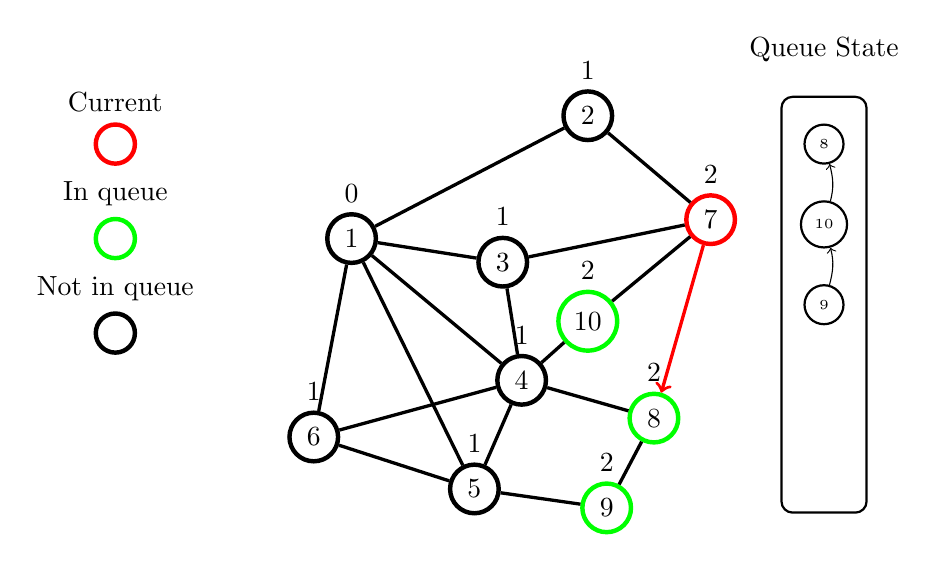
\begin{tikzpicture}[scale=1.2] 
\node[shape=circle, draw=red, 	ultra thick, scale=1.5pt, label={Current}] (U) at (-2.5, 1) {}; 
\node[shape=circle, draw=green,  ultra thick, scale=1.5pt, label={In queue}] (U) at (-2.5, 0) {}; 
\node[shape=circle, draw=black, ultra thick, scale=1.5pt, label={Not in queue}] (U) at (-2.5, -1) {}; 
\draw[thick, rounded corners,draw=black] (4.55, 1.5) rectangle ++(0.9, -1-4*0.85 );
\node[draw=white] at (5, 2) {Queue State} ; 
\node[shape=circle, draw=black, thick, minimum size=2pt] (U0) at (5, 1.0) {\tiny{8}}; 
\node[shape=circle, draw=black, thick, minimum size=2pt] (U1) at (5, 0.15000000000000002) {\tiny{10}}; 
\node[shape=circle, draw=black, thick, minimum size=2pt] (U2) at (5, -0.7) {\tiny{9}}; 
\path[->] (U1) edge [out=75, in=-75] (U0);
\path[->] (U2) edge [out=75, in=-75] (U1);
\node[shape=circle,draw=black, ultra thick, label={$0$}] (1) at (0,0) {1}; 
\node[shape=circle,draw=black, ultra thick, label={$1$}] (2) at (2.5,1.3) {2}; 
\node[shape=circle,draw=black, ultra thick, label={$1$}] (3) at (1.6,-0.25) {3}; 
\node[shape=circle,draw=black, ultra thick, label={$1$}] (4) at (1.8,-1.5) {4}; 
\node[shape=circle,draw=black, ultra thick, label={$1$}] (5) at (1.3,-2.65) {5}; 
\node[shape=circle,draw=black, ultra thick, label={$1$}] (6) at (-0.4,-2.1) {6}; 
\node[shape=circle,draw=red, ultra thick, label={$2$}] (7) at (3.8,0.2) {7}; 
\node[shape=circle,draw=green, ultra thick, label={$2$}] (8) at (3.2,-1.9) {8}; 
\node[shape=circle,draw=green, ultra thick, label={$2$}] (9) at (2.7,-2.85) {9}; 
\node[shape=circle,draw=green, ultra thick, label={$2$}] (10) at (2.5,-0.875) {10}; 
\path [-,very thick, draw=black] (1) edge  (2);
\path [-,very thick, draw=black] (1) edge  (3);
\path [-,very thick, draw=black] (1) edge  (4);
\path [-,very thick, draw=black] (1) edge  (5);
\path [-,very thick, draw=black] (1) edge  (6);
\path [-,very thick, draw=black] (2) edge  (7);
\path [-,very thick, draw=black] (3) edge  (7);
\path [-,very thick, draw=black] (3) edge  (4);
\path [-,very thick, draw=black] (4) edge  (5);
\path [-,very thick, draw=black] (4) edge  (6);
\path [-,very thick, draw=black] (4) edge  (8);
\path [-,very thick, draw=black] (4) edge  (10);
\path [-,very thick, draw=black] (5) edge  (6);
\path [-,very thick, draw=black] (5) edge  (9);
\path [->,very thick, draw=red] (7) edge  (8);
\path [-,very thick, draw=black] (7) edge  (10);
\path [-,very thick, draw=black] (8) edge  (9);
\end{tikzpicture} 
\end{figure} 
\end{frame} 
\begin{frame}{BFS : Example}
\begin{figure}
\vspace*{-1cm} 
\center
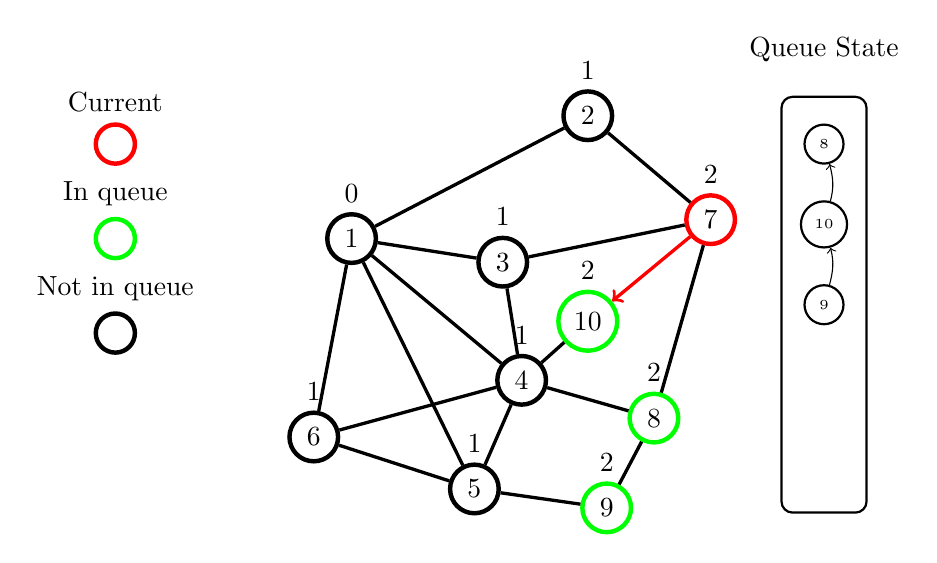
\begin{tikzpicture}[scale=1.2] 
\node[shape=circle, draw=red, 	ultra thick, scale=1.5pt, label={Current}] (U) at (-2.5, 1) {}; 
\node[shape=circle, draw=green,  ultra thick, scale=1.5pt, label={In queue}] (U) at (-2.5, 0) {}; 
\node[shape=circle, draw=black, ultra thick, scale=1.5pt, label={Not in queue}] (U) at (-2.5, -1) {}; 
\draw[thick, rounded corners,draw=black] (4.55, 1.5) rectangle ++(0.9, -1-4*0.85 );
\node[draw=white] at (5, 2) {Queue State} ; 
\node[shape=circle, draw=black, thick, minimum size=2pt] (U0) at (5, 1.0) {\tiny{8}}; 
\node[shape=circle, draw=black, thick, minimum size=2pt] (U1) at (5, 0.15000000000000002) {\tiny{10}}; 
\node[shape=circle, draw=black, thick, minimum size=2pt] (U2) at (5, -0.7) {\tiny{9}}; 
\path[->] (U1) edge [out=75, in=-75] (U0);
\path[->] (U2) edge [out=75, in=-75] (U1);
\node[shape=circle,draw=black, ultra thick, label={$0$}] (1) at (0,0) {1}; 
\node[shape=circle,draw=black, ultra thick, label={$1$}] (2) at (2.5,1.3) {2}; 
\node[shape=circle,draw=black, ultra thick, label={$1$}] (3) at (1.6,-0.25) {3}; 
\node[shape=circle,draw=black, ultra thick, label={$1$}] (4) at (1.8,-1.5) {4}; 
\node[shape=circle,draw=black, ultra thick, label={$1$}] (5) at (1.3,-2.65) {5}; 
\node[shape=circle,draw=black, ultra thick, label={$1$}] (6) at (-0.4,-2.1) {6}; 
\node[shape=circle,draw=red, ultra thick, label={$2$}] (7) at (3.8,0.2) {7}; 
\node[shape=circle,draw=green, ultra thick, label={$2$}] (8) at (3.2,-1.9) {8}; 
\node[shape=circle,draw=green, ultra thick, label={$2$}] (9) at (2.7,-2.85) {9}; 
\node[shape=circle,draw=green, ultra thick, label={$2$}] (10) at (2.5,-0.875) {10}; 
\path [-,very thick, draw=black] (1) edge  (2);
\path [-,very thick, draw=black] (1) edge  (3);
\path [-,very thick, draw=black] (1) edge  (4);
\path [-,very thick, draw=black] (1) edge  (5);
\path [-,very thick, draw=black] (1) edge  (6);
\path [-,very thick, draw=black] (2) edge  (7);
\path [-,very thick, draw=black] (3) edge  (7);
\path [-,very thick, draw=black] (3) edge  (4);
\path [-,very thick, draw=black] (4) edge  (5);
\path [-,very thick, draw=black] (4) edge  (6);
\path [-,very thick, draw=black] (4) edge  (8);
\path [-,very thick, draw=black] (4) edge  (10);
\path [-,very thick, draw=black] (5) edge  (6);
\path [-,very thick, draw=black] (5) edge  (9);
\path [-,very thick, draw=black] (7) edge  (8);
\path [->,very thick, draw=red] (7) edge  (10);
\path [-,very thick, draw=black] (8) edge  (9);
\end{tikzpicture} 
\end{figure} 
\end{frame} 
\begin{frame}{BFS : Example}
\begin{figure}
\vspace*{-1cm} 
\center
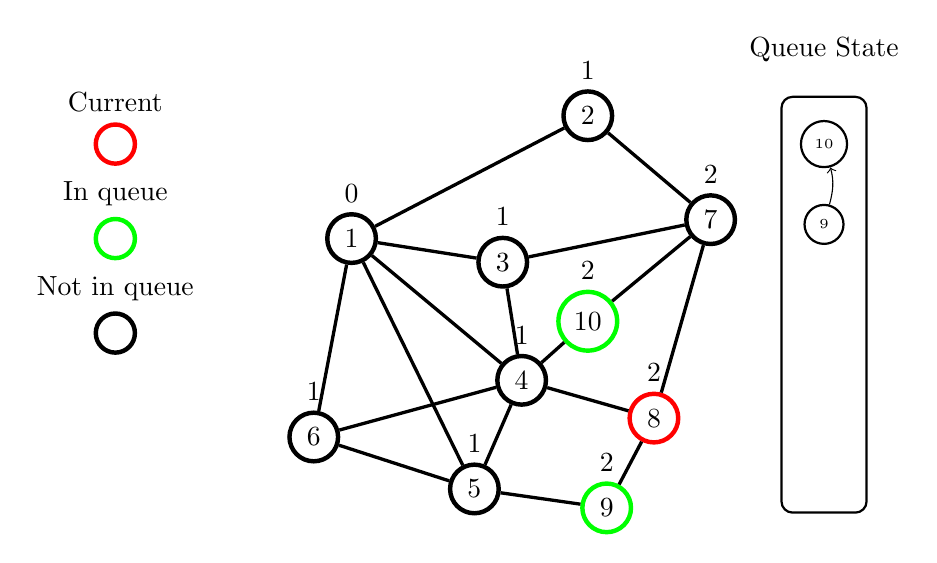
\begin{tikzpicture}[scale=1.2] 
\node[shape=circle, draw=red, 	ultra thick, scale=1.5pt, label={Current}] (U) at (-2.5, 1) {}; 
\node[shape=circle, draw=green,  ultra thick, scale=1.5pt, label={In queue}] (U) at (-2.5, 0) {}; 
\node[shape=circle, draw=black, ultra thick, scale=1.5pt, label={Not in queue}] (U) at (-2.5, -1) {}; 
\draw[thick, rounded corners,draw=black] (4.55, 1.5) rectangle ++(0.9, -1-4*0.85 );
\node[draw=white] at (5, 2) {Queue State} ; 
\node[shape=circle, draw=black, thick, minimum size=2pt] (U0) at (5, 1.0) {\tiny{10}}; 
\node[shape=circle, draw=black, thick, minimum size=2pt] (U1) at (5, 0.15000000000000002) {\tiny{9}}; 
\path[->] (U1) edge [out=75, in=-75] (U0);
\node[shape=circle,draw=black, ultra thick, label={$0$}] (1) at (0,0) {1}; 
\node[shape=circle,draw=black, ultra thick, label={$1$}] (2) at (2.5,1.3) {2}; 
\node[shape=circle,draw=black, ultra thick, label={$1$}] (3) at (1.6,-0.25) {3}; 
\node[shape=circle,draw=black, ultra thick, label={$1$}] (4) at (1.8,-1.5) {4}; 
\node[shape=circle,draw=black, ultra thick, label={$1$}] (5) at (1.3,-2.65) {5}; 
\node[shape=circle,draw=black, ultra thick, label={$1$}] (6) at (-0.4,-2.1) {6}; 
\node[shape=circle,draw=black, ultra thick, label={$2$}] (7) at (3.8,0.2) {7}; 
\node[shape=circle,draw=red, ultra thick, label={$2$}] (8) at (3.2,-1.9) {8}; 
\node[shape=circle,draw=green, ultra thick, label={$2$}] (9) at (2.7,-2.85) {9}; 
\node[shape=circle,draw=green, ultra thick, label={$2$}] (10) at (2.5,-0.875) {10}; 
\path [-,very thick, draw=black] (1) edge  (2);
\path [-,very thick, draw=black] (1) edge  (3);
\path [-,very thick, draw=black] (1) edge  (4);
\path [-,very thick, draw=black] (1) edge  (5);
\path [-,very thick, draw=black] (1) edge  (6);
\path [-,very thick, draw=black] (2) edge  (7);
\path [-,very thick, draw=black] (3) edge  (7);
\path [-,very thick, draw=black] (3) edge  (4);
\path [-,very thick, draw=black] (4) edge  (5);
\path [-,very thick, draw=black] (4) edge  (6);
\path [-,very thick, draw=black] (4) edge  (8);
\path [-,very thick, draw=black] (4) edge  (10);
\path [-,very thick, draw=black] (5) edge  (6);
\path [-,very thick, draw=black] (5) edge  (9);
\path [-,very thick, draw=black] (7) edge  (8);
\path [-,very thick, draw=black] (7) edge  (10);
\path [-,very thick, draw=black] (8) edge  (9);
\end{tikzpicture} 
\end{figure} 
\end{frame} 
\begin{frame}{BFS : Example}
\begin{figure}
\vspace*{-1cm} 
\center
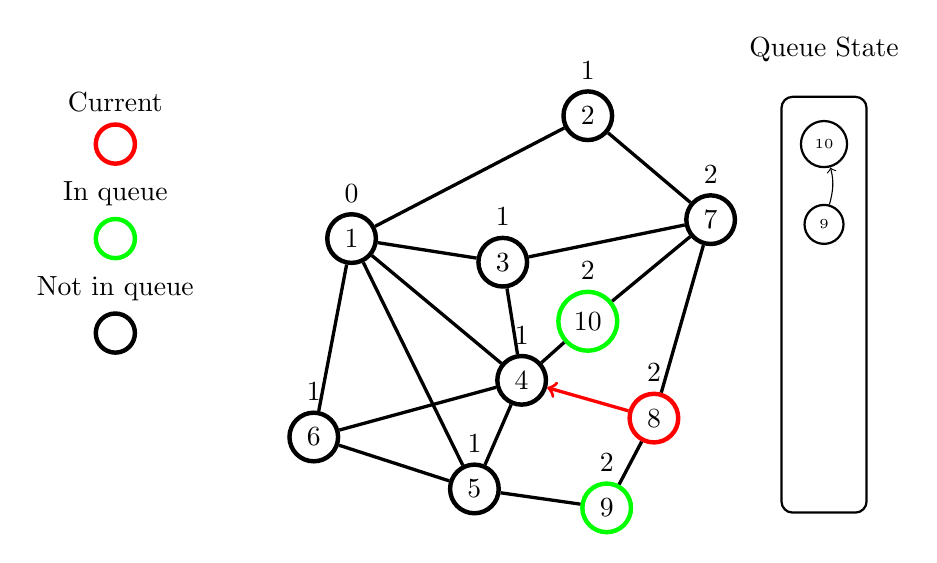
\begin{tikzpicture}[scale=1.2] 
\node[shape=circle, draw=red, 	ultra thick, scale=1.5pt, label={Current}] (U) at (-2.5, 1) {}; 
\node[shape=circle, draw=green,  ultra thick, scale=1.5pt, label={In queue}] (U) at (-2.5, 0) {}; 
\node[shape=circle, draw=black, ultra thick, scale=1.5pt, label={Not in queue}] (U) at (-2.5, -1) {}; 
\draw[thick, rounded corners,draw=black] (4.55, 1.5) rectangle ++(0.9, -1-4*0.85 );
\node[draw=white] at (5, 2) {Queue State} ; 
\node[shape=circle, draw=black, thick, minimum size=2pt] (U0) at (5, 1.0) {\tiny{10}}; 
\node[shape=circle, draw=black, thick, minimum size=2pt] (U1) at (5, 0.15000000000000002) {\tiny{9}}; 
\path[->] (U1) edge [out=75, in=-75] (U0);
\node[shape=circle,draw=black, ultra thick, label={$0$}] (1) at (0,0) {1}; 
\node[shape=circle,draw=black, ultra thick, label={$1$}] (2) at (2.5,1.3) {2}; 
\node[shape=circle,draw=black, ultra thick, label={$1$}] (3) at (1.6,-0.25) {3}; 
\node[shape=circle,draw=black, ultra thick, label={$1$}] (4) at (1.8,-1.5) {4}; 
\node[shape=circle,draw=black, ultra thick, label={$1$}] (5) at (1.3,-2.65) {5}; 
\node[shape=circle,draw=black, ultra thick, label={$1$}] (6) at (-0.4,-2.1) {6}; 
\node[shape=circle,draw=black, ultra thick, label={$2$}] (7) at (3.8,0.2) {7}; 
\node[shape=circle,draw=red, ultra thick, label={$2$}] (8) at (3.2,-1.9) {8}; 
\node[shape=circle,draw=green, ultra thick, label={$2$}] (9) at (2.7,-2.85) {9}; 
\node[shape=circle,draw=green, ultra thick, label={$2$}] (10) at (2.5,-0.875) {10}; 
\path [-,very thick, draw=black] (1) edge  (2);
\path [-,very thick, draw=black] (1) edge  (3);
\path [-,very thick, draw=black] (1) edge  (4);
\path [-,very thick, draw=black] (1) edge  (5);
\path [-,very thick, draw=black] (1) edge  (6);
\path [-,very thick, draw=black] (2) edge  (7);
\path [-,very thick, draw=black] (3) edge  (7);
\path [-,very thick, draw=black] (3) edge  (4);
\path [-,very thick, draw=black] (4) edge  (5);
\path [-,very thick, draw=black] (4) edge  (6);
\path [->,very thick, draw=red] (8) edge  (4);
\path [-,very thick, draw=black] (4) edge  (10);
\path [-,very thick, draw=black] (5) edge  (6);
\path [-,very thick, draw=black] (5) edge  (9);
\path [-,very thick, draw=black] (7) edge  (8);
\path [-,very thick, draw=black] (7) edge  (10);
\path [-,very thick, draw=black] (8) edge  (9);
\end{tikzpicture} 
\end{figure} 
\end{frame} 
\begin{frame}{BFS : Example}
\begin{figure}
\vspace*{-1cm} 
\center
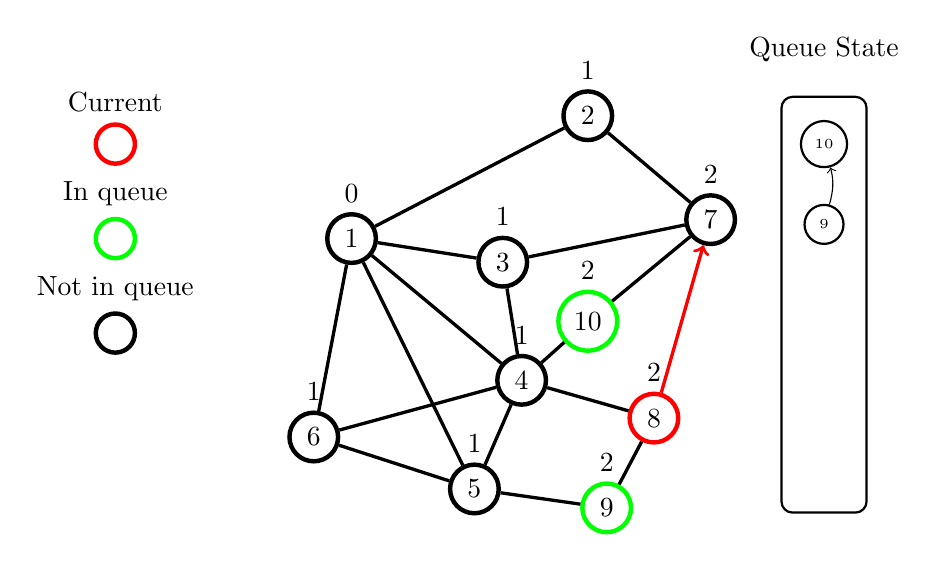
\begin{tikzpicture}[scale=1.2] 
\node[shape=circle, draw=red, 	ultra thick, scale=1.5pt, label={Current}] (U) at (-2.5, 1) {}; 
\node[shape=circle, draw=green,  ultra thick, scale=1.5pt, label={In queue}] (U) at (-2.5, 0) {}; 
\node[shape=circle, draw=black, ultra thick, scale=1.5pt, label={Not in queue}] (U) at (-2.5, -1) {}; 
\draw[thick, rounded corners,draw=black] (4.55, 1.5) rectangle ++(0.9, -1-4*0.85 );
\node[draw=white] at (5, 2) {Queue State} ; 
\node[shape=circle, draw=black, thick, minimum size=2pt] (U0) at (5, 1.0) {\tiny{10}}; 
\node[shape=circle, draw=black, thick, minimum size=2pt] (U1) at (5, 0.15000000000000002) {\tiny{9}}; 
\path[->] (U1) edge [out=75, in=-75] (U0);
\node[shape=circle,draw=black, ultra thick, label={$0$}] (1) at (0,0) {1}; 
\node[shape=circle,draw=black, ultra thick, label={$1$}] (2) at (2.5,1.3) {2}; 
\node[shape=circle,draw=black, ultra thick, label={$1$}] (3) at (1.6,-0.25) {3}; 
\node[shape=circle,draw=black, ultra thick, label={$1$}] (4) at (1.8,-1.5) {4}; 
\node[shape=circle,draw=black, ultra thick, label={$1$}] (5) at (1.3,-2.65) {5}; 
\node[shape=circle,draw=black, ultra thick, label={$1$}] (6) at (-0.4,-2.1) {6}; 
\node[shape=circle,draw=black, ultra thick, label={$2$}] (7) at (3.8,0.2) {7}; 
\node[shape=circle,draw=red, ultra thick, label={$2$}] (8) at (3.2,-1.9) {8}; 
\node[shape=circle,draw=green, ultra thick, label={$2$}] (9) at (2.7,-2.85) {9}; 
\node[shape=circle,draw=green, ultra thick, label={$2$}] (10) at (2.5,-0.875) {10}; 
\path [-,very thick, draw=black] (1) edge  (2);
\path [-,very thick, draw=black] (1) edge  (3);
\path [-,very thick, draw=black] (1) edge  (4);
\path [-,very thick, draw=black] (1) edge  (5);
\path [-,very thick, draw=black] (1) edge  (6);
\path [-,very thick, draw=black] (2) edge  (7);
\path [-,very thick, draw=black] (3) edge  (7);
\path [-,very thick, draw=black] (3) edge  (4);
\path [-,very thick, draw=black] (4) edge  (5);
\path [-,very thick, draw=black] (4) edge  (6);
\path [-,very thick, draw=black] (4) edge  (8);
\path [-,very thick, draw=black] (4) edge  (10);
\path [-,very thick, draw=black] (5) edge  (6);
\path [-,very thick, draw=black] (5) edge  (9);
\path [->,very thick, draw=red] (8) edge  (7);
\path [-,very thick, draw=black] (7) edge  (10);
\path [-,very thick, draw=black] (8) edge  (9);
\end{tikzpicture} 
\end{figure} 
\end{frame} 
\begin{frame}{BFS : Example}
\begin{figure}
\vspace*{-1cm} 
\center
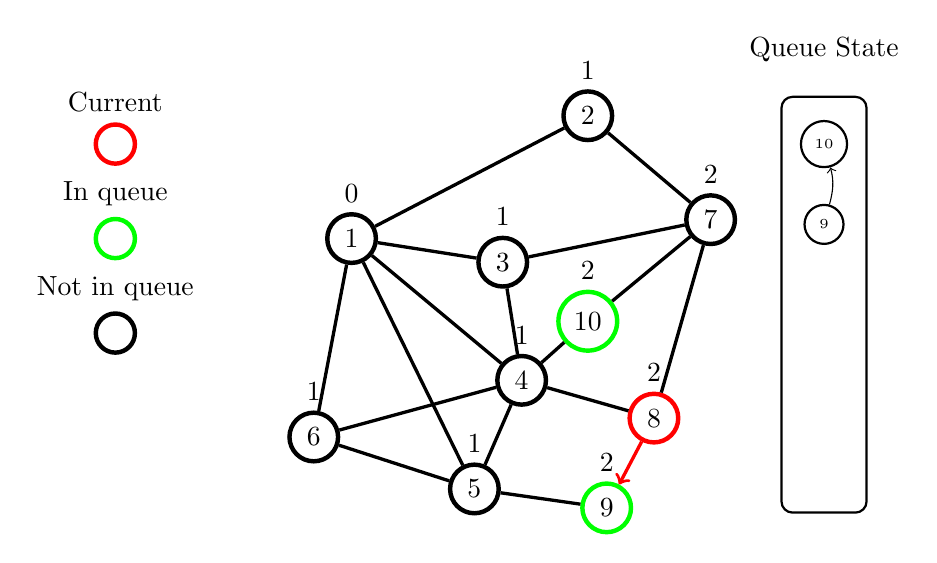
\begin{tikzpicture}[scale=1.2] 
\node[shape=circle, draw=red, 	ultra thick, scale=1.5pt, label={Current}] (U) at (-2.5, 1) {}; 
\node[shape=circle, draw=green,  ultra thick, scale=1.5pt, label={In queue}] (U) at (-2.5, 0) {}; 
\node[shape=circle, draw=black, ultra thick, scale=1.5pt, label={Not in queue}] (U) at (-2.5, -1) {}; 
\draw[thick, rounded corners,draw=black] (4.55, 1.5) rectangle ++(0.9, -1-4*0.85 );
\node[draw=white] at (5, 2) {Queue State} ; 
\node[shape=circle, draw=black, thick, minimum size=2pt] (U0) at (5, 1.0) {\tiny{10}}; 
\node[shape=circle, draw=black, thick, minimum size=2pt] (U1) at (5, 0.15000000000000002) {\tiny{9}}; 
\path[->] (U1) edge [out=75, in=-75] (U0);
\node[shape=circle,draw=black, ultra thick, label={$0$}] (1) at (0,0) {1}; 
\node[shape=circle,draw=black, ultra thick, label={$1$}] (2) at (2.5,1.3) {2}; 
\node[shape=circle,draw=black, ultra thick, label={$1$}] (3) at (1.6,-0.25) {3}; 
\node[shape=circle,draw=black, ultra thick, label={$1$}] (4) at (1.8,-1.5) {4}; 
\node[shape=circle,draw=black, ultra thick, label={$1$}] (5) at (1.3,-2.65) {5}; 
\node[shape=circle,draw=black, ultra thick, label={$1$}] (6) at (-0.4,-2.1) {6}; 
\node[shape=circle,draw=black, ultra thick, label={$2$}] (7) at (3.8,0.2) {7}; 
\node[shape=circle,draw=red, ultra thick, label={$2$}] (8) at (3.2,-1.9) {8}; 
\node[shape=circle,draw=green, ultra thick, label={$2$}] (9) at (2.7,-2.85) {9}; 
\node[shape=circle,draw=green, ultra thick, label={$2$}] (10) at (2.5,-0.875) {10}; 
\path [-,very thick, draw=black] (1) edge  (2);
\path [-,very thick, draw=black] (1) edge  (3);
\path [-,very thick, draw=black] (1) edge  (4);
\path [-,very thick, draw=black] (1) edge  (5);
\path [-,very thick, draw=black] (1) edge  (6);
\path [-,very thick, draw=black] (2) edge  (7);
\path [-,very thick, draw=black] (3) edge  (7);
\path [-,very thick, draw=black] (3) edge  (4);
\path [-,very thick, draw=black] (4) edge  (5);
\path [-,very thick, draw=black] (4) edge  (6);
\path [-,very thick, draw=black] (4) edge  (8);
\path [-,very thick, draw=black] (4) edge  (10);
\path [-,very thick, draw=black] (5) edge  (6);
\path [-,very thick, draw=black] (5) edge  (9);
\path [-,very thick, draw=black] (7) edge  (8);
\path [-,very thick, draw=black] (7) edge  (10);
\path [->,very thick, draw=red] (8) edge  (9);
\end{tikzpicture} 
\end{figure} 
\end{frame} 
\begin{frame}{BFS : Example}
\begin{figure}
\vspace*{-1cm} 
\center
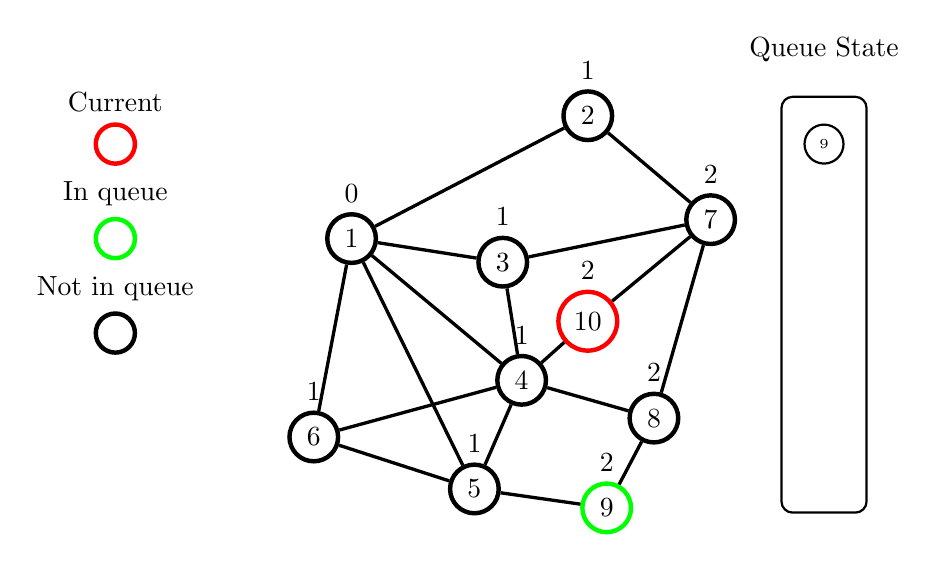
\begin{tikzpicture}[scale=1.2] 
\node[shape=circle, draw=red, 	ultra thick, scale=1.5pt, label={Current}] (U) at (-2.5, 1) {}; 
\node[shape=circle, draw=green,  ultra thick, scale=1.5pt, label={In queue}] (U) at (-2.5, 0) {}; 
\node[shape=circle, draw=black, ultra thick, scale=1.5pt, label={Not in queue}] (U) at (-2.5, -1) {}; 
\draw[thick, rounded corners,draw=black] (4.55, 1.5) rectangle ++(0.9, -1-4*0.85 );
\node[draw=white] at (5, 2) {Queue State} ; 
\node[shape=circle, draw=black, thick, minimum size=2pt] (U0) at (5, 1.0) {\tiny{9}}; 
\node[shape=circle,draw=black, ultra thick, label={$0$}] (1) at (0,0) {1}; 
\node[shape=circle,draw=black, ultra thick, label={$1$}] (2) at (2.5,1.3) {2}; 
\node[shape=circle,draw=black, ultra thick, label={$1$}] (3) at (1.6,-0.25) {3}; 
\node[shape=circle,draw=black, ultra thick, label={$1$}] (4) at (1.8,-1.5) {4}; 
\node[shape=circle,draw=black, ultra thick, label={$1$}] (5) at (1.3,-2.65) {5}; 
\node[shape=circle,draw=black, ultra thick, label={$1$}] (6) at (-0.4,-2.1) {6}; 
\node[shape=circle,draw=black, ultra thick, label={$2$}] (7) at (3.8,0.2) {7}; 
\node[shape=circle,draw=black, ultra thick, label={$2$}] (8) at (3.2,-1.9) {8}; 
\node[shape=circle,draw=green, ultra thick, label={$2$}] (9) at (2.7,-2.85) {9}; 
\node[shape=circle,draw=red, ultra thick, label={$2$}] (10) at (2.5,-0.875) {10}; 
\path [-,very thick, draw=black] (1) edge  (2);
\path [-,very thick, draw=black] (1) edge  (3);
\path [-,very thick, draw=black] (1) edge  (4);
\path [-,very thick, draw=black] (1) edge  (5);
\path [-,very thick, draw=black] (1) edge  (6);
\path [-,very thick, draw=black] (2) edge  (7);
\path [-,very thick, draw=black] (3) edge  (7);
\path [-,very thick, draw=black] (3) edge  (4);
\path [-,very thick, draw=black] (4) edge  (5);
\path [-,very thick, draw=black] (4) edge  (6);
\path [-,very thick, draw=black] (4) edge  (8);
\path [-,very thick, draw=black] (4) edge  (10);
\path [-,very thick, draw=black] (5) edge  (6);
\path [-,very thick, draw=black] (5) edge  (9);
\path [-,very thick, draw=black] (7) edge  (8);
\path [-,very thick, draw=black] (7) edge  (10);
\path [-,very thick, draw=black] (8) edge  (9);
\end{tikzpicture} 
\end{figure} 
\end{frame} 
\begin{frame}{BFS : Example}
\begin{figure}
\vspace*{-1cm} 
\center
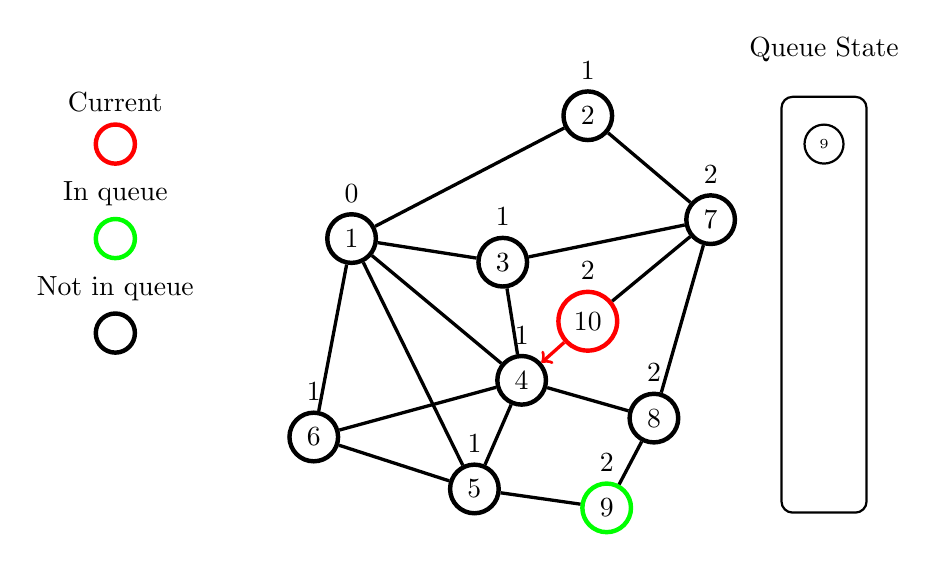
\begin{tikzpicture}[scale=1.2] 
\node[shape=circle, draw=red, 	ultra thick, scale=1.5pt, label={Current}] (U) at (-2.5, 1) {}; 
\node[shape=circle, draw=green,  ultra thick, scale=1.5pt, label={In queue}] (U) at (-2.5, 0) {}; 
\node[shape=circle, draw=black, ultra thick, scale=1.5pt, label={Not in queue}] (U) at (-2.5, -1) {}; 
\draw[thick, rounded corners,draw=black] (4.55, 1.5) rectangle ++(0.9, -1-4*0.85 );
\node[draw=white] at (5, 2) {Queue State} ; 
\node[shape=circle, draw=black, thick, minimum size=2pt] (U0) at (5, 1.0) {\tiny{9}}; 
\node[shape=circle,draw=black, ultra thick, label={$0$}] (1) at (0,0) {1}; 
\node[shape=circle,draw=black, ultra thick, label={$1$}] (2) at (2.5,1.3) {2}; 
\node[shape=circle,draw=black, ultra thick, label={$1$}] (3) at (1.6,-0.25) {3}; 
\node[shape=circle,draw=black, ultra thick, label={$1$}] (4) at (1.8,-1.5) {4}; 
\node[shape=circle,draw=black, ultra thick, label={$1$}] (5) at (1.3,-2.65) {5}; 
\node[shape=circle,draw=black, ultra thick, label={$1$}] (6) at (-0.4,-2.1) {6}; 
\node[shape=circle,draw=black, ultra thick, label={$2$}] (7) at (3.8,0.2) {7}; 
\node[shape=circle,draw=black, ultra thick, label={$2$}] (8) at (3.2,-1.9) {8}; 
\node[shape=circle,draw=green, ultra thick, label={$2$}] (9) at (2.7,-2.85) {9}; 
\node[shape=circle,draw=red, ultra thick, label={$2$}] (10) at (2.5,-0.875) {10}; 
\path [-,very thick, draw=black] (1) edge  (2);
\path [-,very thick, draw=black] (1) edge  (3);
\path [-,very thick, draw=black] (1) edge  (4);
\path [-,very thick, draw=black] (1) edge  (5);
\path [-,very thick, draw=black] (1) edge  (6);
\path [-,very thick, draw=black] (2) edge  (7);
\path [-,very thick, draw=black] (3) edge  (7);
\path [-,very thick, draw=black] (3) edge  (4);
\path [-,very thick, draw=black] (4) edge  (5);
\path [-,very thick, draw=black] (4) edge  (6);
\path [-,very thick, draw=black] (4) edge  (8);
\path [->,very thick, draw=red] (10) edge  (4);
\path [-,very thick, draw=black] (5) edge  (6);
\path [-,very thick, draw=black] (5) edge  (9);
\path [-,very thick, draw=black] (7) edge  (8);
\path [-,very thick, draw=black] (7) edge  (10);
\path [-,very thick, draw=black] (8) edge  (9);
\end{tikzpicture} 
\end{figure} 
\end{frame} 
\begin{frame}{BFS : Example}
\begin{figure}
\vspace*{-1cm} 
\center
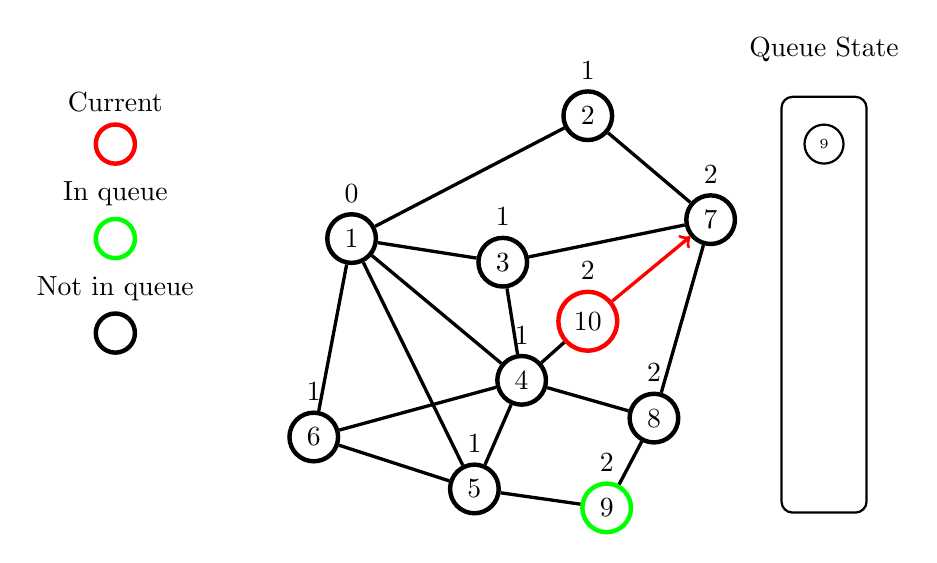
\begin{tikzpicture}[scale=1.2] 
\node[shape=circle, draw=red, 	ultra thick, scale=1.5pt, label={Current}] (U) at (-2.5, 1) {}; 
\node[shape=circle, draw=green,  ultra thick, scale=1.5pt, label={In queue}] (U) at (-2.5, 0) {}; 
\node[shape=circle, draw=black, ultra thick, scale=1.5pt, label={Not in queue}] (U) at (-2.5, -1) {}; 
\draw[thick, rounded corners,draw=black] (4.55, 1.5) rectangle ++(0.9, -1-4*0.85 );
\node[draw=white] at (5, 2) {Queue State} ; 
\node[shape=circle, draw=black, thick, minimum size=2pt] (U0) at (5, 1.0) {\tiny{9}}; 
\node[shape=circle,draw=black, ultra thick, label={$0$}] (1) at (0,0) {1}; 
\node[shape=circle,draw=black, ultra thick, label={$1$}] (2) at (2.5,1.3) {2}; 
\node[shape=circle,draw=black, ultra thick, label={$1$}] (3) at (1.6,-0.25) {3}; 
\node[shape=circle,draw=black, ultra thick, label={$1$}] (4) at (1.8,-1.5) {4}; 
\node[shape=circle,draw=black, ultra thick, label={$1$}] (5) at (1.3,-2.65) {5}; 
\node[shape=circle,draw=black, ultra thick, label={$1$}] (6) at (-0.4,-2.1) {6}; 
\node[shape=circle,draw=black, ultra thick, label={$2$}] (7) at (3.8,0.2) {7}; 
\node[shape=circle,draw=black, ultra thick, label={$2$}] (8) at (3.2,-1.9) {8}; 
\node[shape=circle,draw=green, ultra thick, label={$2$}] (9) at (2.7,-2.85) {9}; 
\node[shape=circle,draw=red, ultra thick, label={$2$}] (10) at (2.5,-0.875) {10}; 
\path [-,very thick, draw=black] (1) edge  (2);
\path [-,very thick, draw=black] (1) edge  (3);
\path [-,very thick, draw=black] (1) edge  (4);
\path [-,very thick, draw=black] (1) edge  (5);
\path [-,very thick, draw=black] (1) edge  (6);
\path [-,very thick, draw=black] (2) edge  (7);
\path [-,very thick, draw=black] (3) edge  (7);
\path [-,very thick, draw=black] (3) edge  (4);
\path [-,very thick, draw=black] (4) edge  (5);
\path [-,very thick, draw=black] (4) edge  (6);
\path [-,very thick, draw=black] (4) edge  (8);
\path [-,very thick, draw=black] (4) edge  (10);
\path [-,very thick, draw=black] (5) edge  (6);
\path [-,very thick, draw=black] (5) edge  (9);
\path [-,very thick, draw=black] (7) edge  (8);
\path [->,very thick, draw=red] (10) edge  (7);
\path [-,very thick, draw=black] (8) edge  (9);
\end{tikzpicture} 
\end{figure} 
\end{frame} 
\begin{frame}{BFS : Example}
\begin{figure}
\vspace*{-1cm} 
\center
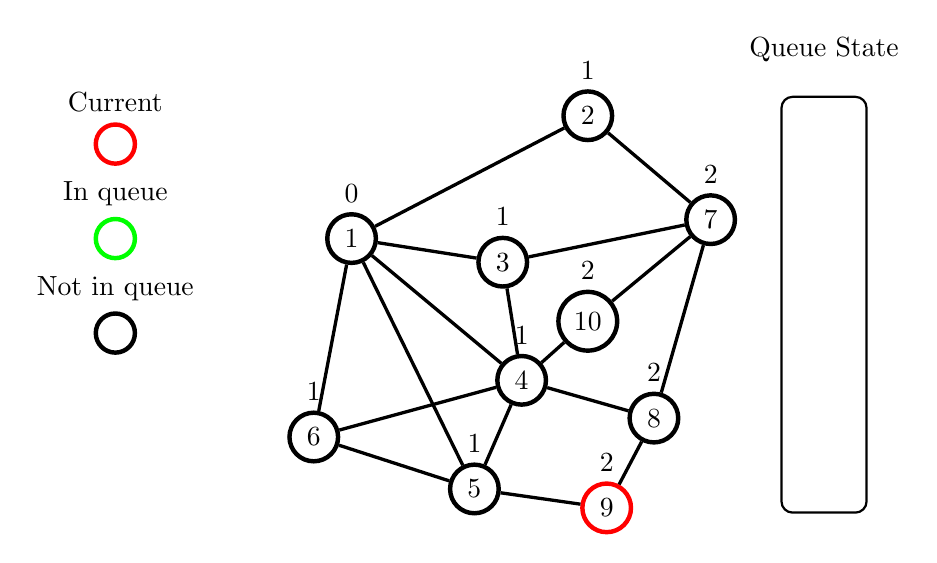
\begin{tikzpicture}[scale=1.2] 
\node[shape=circle, draw=red, 	ultra thick, scale=1.5pt, label={Current}] (U) at (-2.5, 1) {}; 
\node[shape=circle, draw=green,  ultra thick, scale=1.5pt, label={In queue}] (U) at (-2.5, 0) {}; 
\node[shape=circle, draw=black, ultra thick, scale=1.5pt, label={Not in queue}] (U) at (-2.5, -1) {}; 
\draw[thick, rounded corners,draw=black] (4.55, 1.5) rectangle ++(0.9, -1-4*0.85 );
\node[draw=white] at (5, 2) {Queue State} ; 
\node[shape=circle,draw=black, ultra thick, label={$0$}] (1) at (0,0) {1}; 
\node[shape=circle,draw=black, ultra thick, label={$1$}] (2) at (2.5,1.3) {2}; 
\node[shape=circle,draw=black, ultra thick, label={$1$}] (3) at (1.6,-0.25) {3}; 
\node[shape=circle,draw=black, ultra thick, label={$1$}] (4) at (1.8,-1.5) {4}; 
\node[shape=circle,draw=black, ultra thick, label={$1$}] (5) at (1.3,-2.65) {5}; 
\node[shape=circle,draw=black, ultra thick, label={$1$}] (6) at (-0.4,-2.1) {6}; 
\node[shape=circle,draw=black, ultra thick, label={$2$}] (7) at (3.8,0.2) {7}; 
\node[shape=circle,draw=black, ultra thick, label={$2$}] (8) at (3.2,-1.9) {8}; 
\node[shape=circle,draw=red, ultra thick, label={$2$}] (9) at (2.7,-2.85) {9}; 
\node[shape=circle,draw=black, ultra thick, label={$2$}] (10) at (2.5,-0.875) {10}; 
\path [-,very thick, draw=black] (1) edge  (2);
\path [-,very thick, draw=black] (1) edge  (3);
\path [-,very thick, draw=black] (1) edge  (4);
\path [-,very thick, draw=black] (1) edge  (5);
\path [-,very thick, draw=black] (1) edge  (6);
\path [-,very thick, draw=black] (2) edge  (7);
\path [-,very thick, draw=black] (3) edge  (7);
\path [-,very thick, draw=black] (3) edge  (4);
\path [-,very thick, draw=black] (4) edge  (5);
\path [-,very thick, draw=black] (4) edge  (6);
\path [-,very thick, draw=black] (4) edge  (8);
\path [-,very thick, draw=black] (4) edge  (10);
\path [-,very thick, draw=black] (5) edge  (6);
\path [-,very thick, draw=black] (5) edge  (9);
\path [-,very thick, draw=black] (7) edge  (8);
\path [-,very thick, draw=black] (7) edge  (10);
\path [-,very thick, draw=black] (8) edge  (9);
\end{tikzpicture} 
\end{figure} 
\end{frame} 
\begin{frame}{BFS : Example}
\begin{figure}
\vspace*{-1cm} 
\center
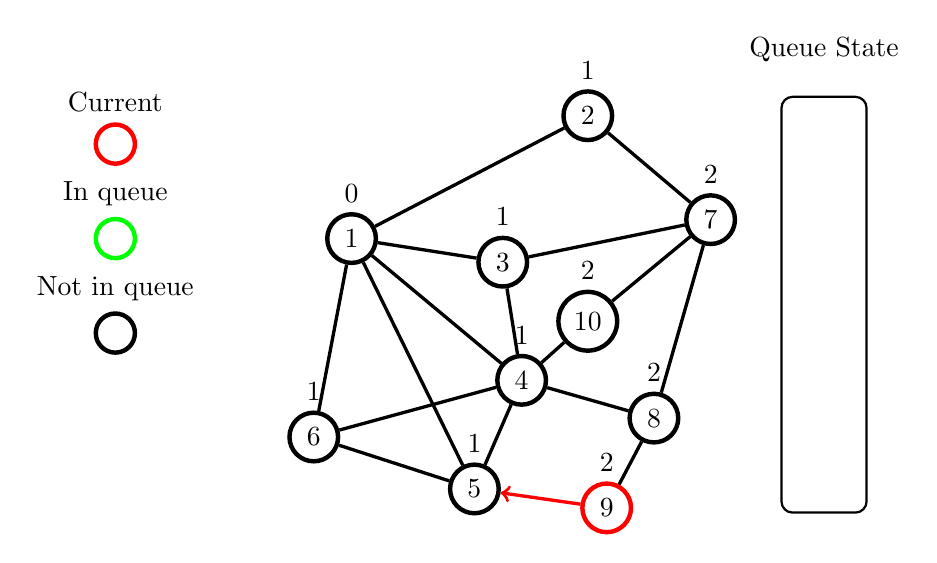
\begin{tikzpicture}[scale=1.2] 
\node[shape=circle, draw=red, 	ultra thick, scale=1.5pt, label={Current}] (U) at (-2.5, 1) {}; 
\node[shape=circle, draw=green,  ultra thick, scale=1.5pt, label={In queue}] (U) at (-2.5, 0) {}; 
\node[shape=circle, draw=black, ultra thick, scale=1.5pt, label={Not in queue}] (U) at (-2.5, -1) {}; 
\draw[thick, rounded corners,draw=black] (4.55, 1.5) rectangle ++(0.9, -1-4*0.85 );
\node[draw=white] at (5, 2) {Queue State} ; 
\node[shape=circle,draw=black, ultra thick, label={$0$}] (1) at (0,0) {1}; 
\node[shape=circle,draw=black, ultra thick, label={$1$}] (2) at (2.5,1.3) {2}; 
\node[shape=circle,draw=black, ultra thick, label={$1$}] (3) at (1.6,-0.25) {3}; 
\node[shape=circle,draw=black, ultra thick, label={$1$}] (4) at (1.8,-1.5) {4}; 
\node[shape=circle,draw=black, ultra thick, label={$1$}] (5) at (1.3,-2.65) {5}; 
\node[shape=circle,draw=black, ultra thick, label={$1$}] (6) at (-0.4,-2.1) {6}; 
\node[shape=circle,draw=black, ultra thick, label={$2$}] (7) at (3.8,0.2) {7}; 
\node[shape=circle,draw=black, ultra thick, label={$2$}] (8) at (3.2,-1.9) {8}; 
\node[shape=circle,draw=red, ultra thick, label={$2$}] (9) at (2.7,-2.85) {9}; 
\node[shape=circle,draw=black, ultra thick, label={$2$}] (10) at (2.5,-0.875) {10}; 
\path [-,very thick, draw=black] (1) edge  (2);
\path [-,very thick, draw=black] (1) edge  (3);
\path [-,very thick, draw=black] (1) edge  (4);
\path [-,very thick, draw=black] (1) edge  (5);
\path [-,very thick, draw=black] (1) edge  (6);
\path [-,very thick, draw=black] (2) edge  (7);
\path [-,very thick, draw=black] (3) edge  (7);
\path [-,very thick, draw=black] (3) edge  (4);
\path [-,very thick, draw=black] (4) edge  (5);
\path [-,very thick, draw=black] (4) edge  (6);
\path [-,very thick, draw=black] (4) edge  (8);
\path [-,very thick, draw=black] (4) edge  (10);
\path [-,very thick, draw=black] (5) edge  (6);
\path [->,very thick, draw=red] (9) edge  (5);
\path [-,very thick, draw=black] (7) edge  (8);
\path [-,very thick, draw=black] (7) edge  (10);
\path [-,very thick, draw=black] (8) edge  (9);
\end{tikzpicture} 
\end{figure} 
\end{frame} 
\begin{frame}{BFS : Example}
\begin{figure}
\vspace*{-1cm} 
\center
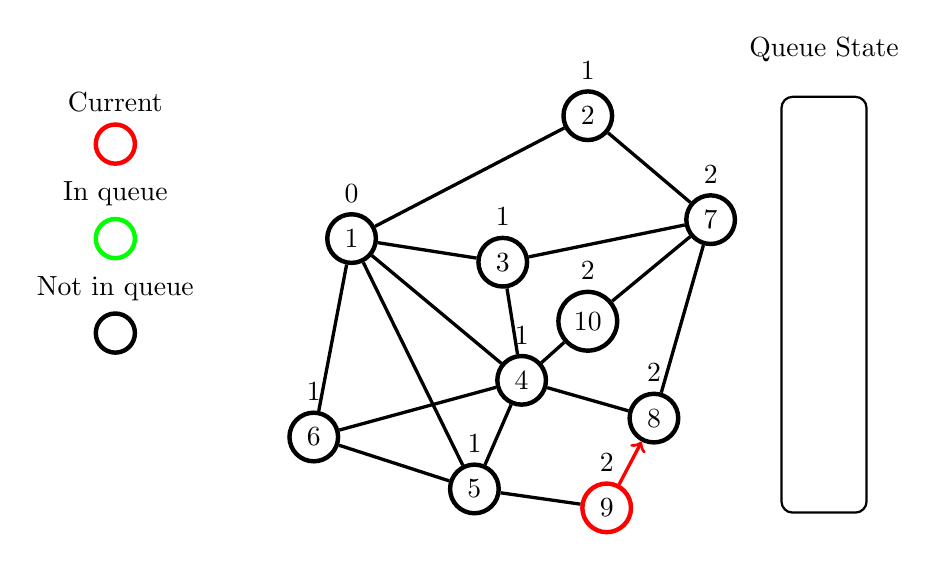
\begin{tikzpicture}[scale=1.2] 
\node[shape=circle, draw=red, 	ultra thick, scale=1.5pt, label={Current}] (U) at (-2.5, 1) {}; 
\node[shape=circle, draw=green,  ultra thick, scale=1.5pt, label={In queue}] (U) at (-2.5, 0) {}; 
\node[shape=circle, draw=black, ultra thick, scale=1.5pt, label={Not in queue}] (U) at (-2.5, -1) {}; 
\draw[thick, rounded corners,draw=black] (4.55, 1.5) rectangle ++(0.9, -1-4*0.85 );
\node[draw=white] at (5, 2) {Queue State} ; 
\node[shape=circle,draw=black, ultra thick, label={$0$}] (1) at (0,0) {1}; 
\node[shape=circle,draw=black, ultra thick, label={$1$}] (2) at (2.5,1.3) {2}; 
\node[shape=circle,draw=black, ultra thick, label={$1$}] (3) at (1.6,-0.25) {3}; 
\node[shape=circle,draw=black, ultra thick, label={$1$}] (4) at (1.8,-1.5) {4}; 
\node[shape=circle,draw=black, ultra thick, label={$1$}] (5) at (1.3,-2.65) {5}; 
\node[shape=circle,draw=black, ultra thick, label={$1$}] (6) at (-0.4,-2.1) {6}; 
\node[shape=circle,draw=black, ultra thick, label={$2$}] (7) at (3.8,0.2) {7}; 
\node[shape=circle,draw=black, ultra thick, label={$2$}] (8) at (3.2,-1.9) {8}; 
\node[shape=circle,draw=red, ultra thick, label={$2$}] (9) at (2.7,-2.85) {9}; 
\node[shape=circle,draw=black, ultra thick, label={$2$}] (10) at (2.5,-0.875) {10}; 
\path [-,very thick, draw=black] (1) edge  (2);
\path [-,very thick, draw=black] (1) edge  (3);
\path [-,very thick, draw=black] (1) edge  (4);
\path [-,very thick, draw=black] (1) edge  (5);
\path [-,very thick, draw=black] (1) edge  (6);
\path [-,very thick, draw=black] (2) edge  (7);
\path [-,very thick, draw=black] (3) edge  (7);
\path [-,very thick, draw=black] (3) edge  (4);
\path [-,very thick, draw=black] (4) edge  (5);
\path [-,very thick, draw=black] (4) edge  (6);
\path [-,very thick, draw=black] (4) edge  (8);
\path [-,very thick, draw=black] (4) edge  (10);
\path [-,very thick, draw=black] (5) edge  (6);
\path [-,very thick, draw=black] (5) edge  (9);
\path [-,very thick, draw=black] (7) edge  (8);
\path [-,very thick, draw=black] (7) edge  (10);
\path [->,very thick, draw=red] (9) edge  (8);
\end{tikzpicture} 
\end{figure} 
\end{frame} 
